
% to choose your degree
% please un-comment just one of the following
\documentclass[bsc,frontabs,twoside,singlespacing,parskip,deptreport]{infthesis}     % for BSc, BEng etc.
% \documentclass[minf,frontabs,twoside,singlespacing,parskip,deptreport]{infthesis}  % for MInf

\usepackage{pdfpages}
\usepackage{float}% If comment this, figure moves to Page 2
\usepackage{subcaption}
\usepackage{tabulary}
\usepackage{listings}
\usepackage{ wasysym }
%\usepackage{hyperref}

% This is for the Verbatim package
\usepackage{fancyvrb}
\usepackage{bera}



\usepackage[toc,page]{appendix}

\begin{document}

\title{Finding Vulnerabilities in Low-Level Protocols}

\author{Nordine Saadouni}

% to choose your course
% please un-comment just one of the following
%\course{Artificial Intelligence and Computer Science}
%\course{Artificial Intelligence and Software Engineering}
%\course{Artificial Intelligence and Mathematics}
%\course{Artificial Intelligence and Psychology }   
%\course{Artificial Intelligence with Psychology }   
%\course{Linguistics and Artificial Intelligence}    
\course{Computer Science}
%\course{Software Engineering}
%\course{Computer Science and Electronics}    
%\course{Electronics and Software Engineering}    
%\course{Computer Science and Management Science}    
%\course{Computer Science and Mathematics}
%\course{Computer Science and Physics}  
%\course{Computer Science and Statistics}    

% to choose your report type
% please un-comment just one of the following
%\project{Undergraduate Dissertation} % CS&E, E&SE, AI&L
%\project{Undergraduate Thesis} % AI%Psy
\project{4th Year Project Report}

\date{\today}


\abstract{
Basic example of an abstract (this will be changed)\\

Smartcards are used commercially and within industry for authentication, encryption, decryption, signing and verifying data. This paper aims to look into how the smartcard interacts with an application at the lower level. PKCS\#11 (public key cryptography system?) is the standard that is implemented at the higher level and then broken down into command/response pairs sent as APDU traffic to and from the smart card. It is the APDU low-level protocol that will be analysed to see if any vulnerabilities are present with regard to the smart cards tested.\\
}

\maketitle


\section*{Acknowledgements}
Acknowledgements go here.
% Myrto, Andriana, Parents
% MSC student? 

\tableofcontents

%\pagenumbering{arabic}

%---------------------------------------------------------------------------------------------------------------------------------------------------

\chapter{Introduction}
Smartcards are formally known as integrated circuit cards (ICC), and are universally thought to be secure, tamper-resistant devices. They store and process, cryptographic keys, authentication and user sensitive data. They are utilised to preform operations where confidentiality, data integrity and authentication are key to the security of a system.\\

Smartcards offer what seems to be more secure methods for using cryptographic operations. (And should still provide the same level of security that would be offered to un-compromised systems, compared to those that are compromised by an attacker). This is partly due to the fact that the majority of modern smartcards have their own on-board micro-controller, to allow all of these operations to take place on the smartcard itself, with keys that are unknown to the outside world and stored securely on the device. Meaning the only actor that should be able to preform such operations would need to be in possession of the smartcard and the PIN/password. In many industries, for applications such as, banking/ payment systems, telecommunications, healthcare and public sector transport, smartcards are used due to the security they are believed to provide.

The most common API (application programming interface) that is used to communicate with smartcards is the RSA defined PKCS\#11 (Public Key Cryptography Standard). Also known as 'Cryptoki' (cryptographic token interface, pronounced as 'crypto-key'). The standard defines a platform-independent API to smartcards and hardware security modules (HSM). PKCS\#11 originated from RSA security, but has since been placed into the hands of OASIS PKCS\#11 Technical Committee to continue its work (since 2013). [reference wikipedia PKCS\#11].\\


In the previous 10-15 years, literature has shown a great deal of research into the examination of the PKCS\#11 API, and the security it provides. Yet little attention has been paid to that of the lower-level communication (command-response pairs), in which the higher level API is broken down into. It is this area that we wish to research within this paper. The reasoning is simple. If we cannot trust the security of the low-level commands that implement the high level API functions, then in turn we cannot trust the security of the high level API. This is analogous to C code being complied down to binary data to be operated on by the CPU. The addition of two integers cannot be considered correct in C, unless the corresponding binary instructions sent to the CPU are correct as well.  

% maybe not 
The research of the low-level communication will take two forms. 
\begin{enumerate}
\item An analysis of the raw communication between PC and smartcard for all API function calls
\item 
\end{enumerate}


Before we move into the above analysis, supporting material must be introduced. This the rest of this paper will be organized as follows.



%---------------------------------------------------------------------------------------------------------------------------------------------------
\chapter{Background - Cryptography}

This chapter aims to provide an understanding of different cryptographic standards (we do not give explanations regarding the correctness of the standards, merely just how to use them). This is to aid our explanations with regard the smartcards functionality and cryptographic operations used to attempt the secure transfer of sensitive information. In addition this chapter provides an understanding of terminology that is used throughout this paper.

\section{Cryptograhic - Hash Functions}

FIPS PUB 180-4 define [?] hash functions are a one way functions. They take in as input a \textbf{variable sized} message (a string) and output a \textbf{fixed size} message digest (another string). Hash functions should hold three properties:
\begin{enumerate}
\item \textbf{Simple Computation} - It should be easy to calculate the message digest of a given message.
\item \textbf{Difficult Reversing the Computation} - It should be difficult to find the message given its mesage digest.
\item \textbf{Collision Resistance} - It should be difficult to find two messages m$_1$ and m$_2$ that have identical message digests.
\end{enumerate}


$$ Message\_digest = Hash\_function(message) $$


\section{Asymmetric Encryption}

Asymmetric encryption relies on public and private key pairs. Public keys can be sent over insecure channels for an entity to use to encrypt a message. Private keys are to be always kept a secret. Only the private key can be used to decrypt messages encrypted via the public key. This allows communication to remain confidential despite insecure mediums of transport being used.

\subsection{RSA}
Ron Rivest, Adi Shamir, and Leonard Adleman published the RSA asymmetric encryption standard in 1977 [?]. The standard defines a public key (N,e) and a private key (N,d), where N is the multiplication of two large primes p and q. 

\begin{table}[H]
\begin{tabular}{|l|l|l|}
\hline
 & Public Key & Private Key\\
\hline
Modulus & N = p x q & N = p x q\\
\hline
Exponent & e & d\\
\hline
\end{tabular}
\end{table}

Messages to be encrypted are converted into integers to be used for the encryption and decryption process.

\underline{\textbf{RSA public key encryption}}\\
$$ encrpyted\_message =  message^e  \quad mod \quad N $$

\underline{\textbf{RSA private key decryption}}\\
$$ message =  encrypted\_message^d  \quad mod \quad N $$

There are different RSA private and public key pairs. The size of the moudlus (N) in bits gives the names of the different forms of RSA there are. They provide different levels of security. It is suggested to now use RSA-2048 and above.

\begin{table}[H]
\begin{tabular}{|l|c|}
\hline
RSA-type & Exponent size (bytes)\\
\hline
RSA-512 & 64\\
RSA-1024 & 128\\
RSA-2048 & 256\\
RSA-4096 & 512\\
\hline
\end{tabular}
\end{table}

\underline{\textbf{Chinese Remainder Theorem (CRT) RSA cryptography}}\\

G.N.Shinde and H.S.Fadewar published a paper in 2008 [?] explaining how the use of the chienese remainder theorem can improve the efficiency of RSA decryption by upto a factor of four. It required three additional calculations which are the following:
\begin{enumerate}
\item $dP = (1/e)\quad  mod (p-1)$
\item $dQ = (1/e) \quad mod (q-1)$
\item $qInv = (1/q) \quad mod (p)$
\end{enumerate}

To compute the decryption ($m= c^d mod(N)$) using CRT, we do the following:
$$m1 = c^{dP} mod p$$
$$m2 = c^{dQ} mod q$$
$$h = qInv.(m1 - m2) mod (p)$$
$$ m = m2 + h.q  == c^d mod (N)$$


\subsection{Diffie Hellman}
Whitfield Diffie and Martin Hellman published in 1976 [?] the Diffie Hellman protocol. The protocol again has a public and private key pair that is used to derive a shared secret over an insecure channel. Two entities must agree on the global parameters.

\begin{table}[H]
\begin{tabular}{|l|c|}
\hline
 & Global Parameter\\
\hline
Generator & \textit{G}\\
\hline
Public Modulus & \textit{p}\\
\hline
\end{tabular}
\end{table}

Using the global parameters each entity generates selects its own private key to be a random number between 1 and \textit{p-1}. And then calculate their respective public keys as follows:
$$ public\_key = G^{private\_key} \quad mod (p)$$

The 2 entities send each other their public keys over the insecure channel, and can then calculate a shared secret (that other entities that cannot calculate) as follows:
$$ shared\_secret = public\_key_2^{private\_key_1} \quad mod (p) $$

\subsection{Elliptic Curve Cryptography}
\textit{[Note, we only report how ECCDH operates as this is an area we research within chapter 7 as part of an attack.]}

Elliptic curve cryptography is based on the algebraic structure of elliptic curve over finite fields. The standard only received wide spread use starting 2004. It is similar to RSA in the respect that it provides a method for sharing an entities public key over and insecure channel. The public key can be used to encrypt data, sign data or even use a version of the Diffie Hellman protocol to derive a shared secret (ECCDH). Certicom Research published a revised paper in 2009 [?] explaining how to use the ECC standard.

One major difference between ECC and standard cryptographic methods, is the addition and multiplication operations. In elliptic curve cryptograhpy addition and multiplication are redefined over the curve. The maths behind ECC means that addition and multiplication are no longer reversiable operations, and are now assumed to be one way functions. In which to compute the reverse of one of the operations, one must solve the 'elliptic curve discrete logarithm problem'. We report below in figure 2.1 examples of how multiplication and addition operation work in ECC.
% IMAGE: ECC addition and multiplication
\begin{figure}[H]
\centering
\begin{subfigure}{1.2\textwidth}
  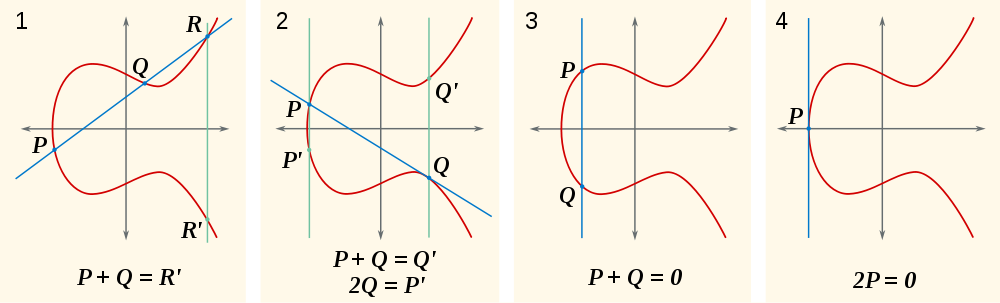
\includegraphics[width=1\linewidth]
  {images/crypto/ecc.png}
\end{subfigure}
\caption{ECC Addition and Multiplication [?]}
\end{figure}

Global Paramters are shared (similar to Diffie Hellman) between two entities, these are:
\begin{table}[H]
\begin{tabular}{|l|l|}
\hline
Global Parameter & Description\\
\hline
\textit{p} & The field the curve is defined over\\
\hline
\textit{(a,b)} & Values defining the curve\\
\hline
\textit{G} & Generator point (fixed point on the curve)\\
\hline
\textit{n} & Prime order of G (n.G = elliptic identity)\\
\hline
\textit{h} & Cofactor\\
\hline
\textit{Seed} & Random number\\
\hline
\end{tabular}
\end{table}

\underline{\textbf{Elliptic Curve Cofactor Diffie Hellman}}\\

Using the global parameters two entities can now generate their own private keys (defined on the curve). The value of their respective private keys (\textit{d}), are randomly selected numbers (seeded with \textit{Seed}), in the range $ 1 <= d <= (n-1)$.

With their private keys each entity can now calculate their own public keys to send to one and other. This is similar to Diffie Hellman, however the ECC multiplication operation is used instead.

\textit{public\_key$_1$ = (X$_1$, Y$_1$) - A point on the curve}\\
\textit{public\_key$_1$ = (private\_key$_1$).G}\\

Once each entity has each others public keys, they can now calculate a shared secret using the following formula:

\begin{center}
\textit{shared\_secret = public\_key$_2$.(private\_key$_1$.h)}
\end{center}


\section{Symmetric Encryption}
Symmetric key algorithms rely on the fact that both entities in communication with one and other are both in the knowledge of a shared key. The shared key is to be held a secret by both entities and is used for both encryption and decryption. The symmetric key algorithms that are implemented on the smartcard we analyse are block ciphers. They are named block ciphers due to how the encrypt/ decrypt data, it occurs in blocks (predefined number of bytes). The three block ciphers that the smartcard has implemented are:
\begin{enumerate}
\item Advanced Encryption Standard (AES)
\item Data Encryption Standard (DES)
\item Triple Data encryption Standard (3DES)\\
\end{enumerate}

We have reported the characteristics of the three block ciphers in table 2.1. Block ciphers also have serveral different modes of operation. These modes dictate different methods of encrypting and decrypting data. We have explained the two that are present on the Athena IDprotect smartcard we analyse in this paper.

\begin{table}[H]
\begin{tabular}{|l|c|c|}
\hline
Block Cipher & Block Size (bytes) & Key Size (bytes)\\
\hline
AES-128 & 16 & 16\\
AES-192 & 16 & 24\\
AES-256 & 16 & 32\\
\hline
DES & 8 & 8\\
\hline
3DES-64 & 8 & 8\\
3DES-128 & 8 & 16\\
3DES-192 & 8 & 24\\
\hline
\end{tabular}
\caption{Block Cipher Characteristic's}
\end{table}

% might go against those headings and just list them in the explanations
\subsection{ECB Mode}


% IMAGE: ECB encryption
\begin{figure}[H]
\centering
\begin{subfigure}{1.0\textwidth}
  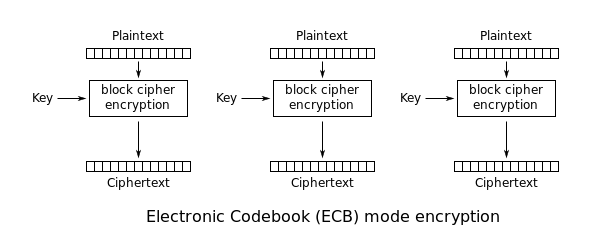
\includegraphics[width=1\linewidth]
  {images/crypto/ecb.png}
\end{subfigure}
\caption{ECC Addition and Multiplication [?]}
\end{figure}
\subsection{CBC Mode}


% IMAGE: CBC encryption
\begin{figure}[H]
\centering
\begin{subfigure}{1.0\textwidth}
  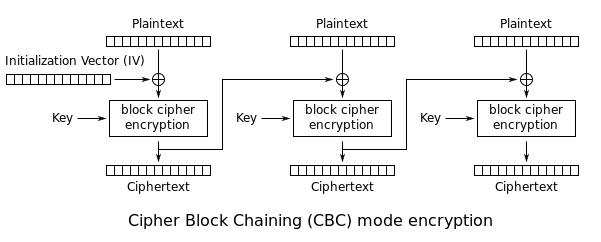
\includegraphics[width=1\linewidth]
  {images/crypto/cbc.png}
\end{subfigure}
\caption{ECC Addition and Multiplication [?]}
\end{figure}

\section{Message Authentication Codes}

\noindent explain what a message authentication code is, what its used for\\
\noindent (wikipedia have good diagrams and explanations of this!!)

\subsection{Hash Based - Message Authentication Codes (HMAC)}
\subsection{Cryptographic Based - Message Authentication Codes (CMAC)}

\section{One Time Passwords}

\noindent What is a one time password $\rightarrow$ what forms are there?

\subsection{Hash Based - One Time Passwords (HOTP)}
\subsection{Time Based - One Time Passwords (TOTP)}


%---------------------------------------------------------------------------------------------------------------------------------------------------
\chapter{Background - Standards For Smartcards}

In this chapter we give background knowledge on two essential standards that are required for the use of the contact smartcard we analyse in this paper. These two standards are PKCS\#11 and ISO 7816.

\section{PKCS\#11}
Public Key Cryptography Standard \#11 was created by RSA Laboratories. It is a platform independent API, that defines rules and functions that should be implemented by the card manufacturer in the form of a 'middleware'. The API is written within the C programming language, and only header files are included. The implementation of the API's functions are left to each card vendor, and are required to break down each function into multiple ISO 7816 command-response pairs to carry out the indented function.

Smartcards store cryptographic keys, certificates and data. The standard treats each of these data items as objects. With each object having attributes that define controls that PKCS \#11 API should implement. In sections 2.1.1 and 2.1.2 we report the meanings behind the attributes of PKCS \#11 objects and the PKCS \#11 functions that utilise them.

\pagebreak
\subsection{PKCS \# 11 Object's and Attributes}

There are 5 different types of objects supports by the PKCS \#11 standard. These are presented as the CKA\_class attribute and reported in table 2.1. The sensitive values stored in objects are reported within table 2.1. And finally, the attributes each object has (depending on its type) are reported in table 2.3. The attributes in table 2.3, set controls that the API should implement.

\begin{table}[H]
\begin{tabular}{|l|p{10cm}|}
\hline 
CKA\_class & Definition\\
\hline
Secret Key & A secret key object is an object that stores a block cipher key value and its attributes.\\
\hline
Public Key & A public key object is an object that stores the public key value and attributes of an asymmetric key pair\\
\hline
Private Key & A private key object is an object that stores the private key value and attributes of an asymmetric key pair\\
\hline
Data & A data object is a generic object that allows any value to be stored within its objects value.\\
\hline
Certificate & A certificate object stores certificates usually wrapped in an ASN.1 encoding (e.g X.509) for their use on-line.\\
\hline
\end{tabular}
\caption{PKCS \#11 Object Types}
\end{table}

\begin{table}[H]
\hskip-1.5cm\begin{tabular}{|p{3cm}|p{5cm}|p{10cm}|}
\hline
Object & Value & Definition\\
\hline
Secret Key & CKA\_Value & Stores the value of the block cipher key\\
\hline
Public Key & CKA\_public\_exponent \& CKA\_public\_modulus & Stores the public exponent and modulus of RSA asymmetric keys. (These are different for elliptic curve asymmetric public keys)\\
\hline
Private Key & CKA\_private\_exponent & Stores the private exponent for RSA asymmetric keys. (These are different for elliptic curve asymmetric keys)\\
\hline
Data \& Certificate & CKA\_Value & Stores the value of the data or certificate.\\
\hline
\end{tabular}
\caption{PKCS \#11 Senseitive Attribute Values}
\end{table}

\begin{table}[H]
\begin{tabular}{|l|l|p{10cm}|}
\hline
CKA\_attribute & Value Type & Definition\\
\hline
Key Type & String & The key type attribute defines what type of key the object represents \textbf{\textit{[This is not present for data and certificate objects]}}\\
\hline
Token & Boolean & The token attribute defines whether or not the object is to be stored permanently on the card, or securely destroyed after a session. \textbf{\textit{[If token = True, the object must have an ID]}} \\
\hline

Modulus Bits & Integer & The modulus bits attribute sets the number of bits to use for an RSA asymmetric key pair (E.g. 1024)  \\
\hline
Public Exponent & Integer & The public exponent attribute sets the public exponent for an RSA asymmetric key public key. \\
\hline
Value Length & Integer & The value length attribute sets the key size for a block cipher. (E.g. AES 16 byte or 32 byte key size) \\
\hline

Private & Boolean & The private attribute defines if a user has to be authenticated with the smartcard before the object can be utilised \\
\hline
Label & String & The label attribute gives a name to the object for reference by the user \\
\hline
ID & String & The ID attribute gives an ID string value for lookup searches within the API by the user, when searching for objects stored on the card. \\
\hline
Sensitive & Boolean & The sensitive object defines if an object can be extracted out of the smartcard in an unencrypted format \\
\hline
Extractable & Boolean & The extractable attribute defines if an object can be extracted out of the smartcard\\
\hline
Encrypt & Boolean & The encrypt attribute defines if the object can be used for encrypting data \\
\hline 
Decrypt & Boolean & The decrypt attribute defines if an object can be used for decrypting data \\
\hline
Sign & Boolean & The sign attribute defines if an object can be used for signing data \\
\hline 
Verify & Boolean & The verify attribute defines if an object can be used for verifying the signature of data \\
\hline
Wrap & Boolean & The wrap attribute defines if an object can be used for wrapping (encrypting) another key object for extraction out of the smartcard in an encrypted format \\
\hline
Unwrap & Boolean & The unwrap attribute defines if an object can be used for unwrapping (decrypting) another (encrypted) key object for storing within the smartcard \\
\hline
\end{tabular}
\caption{PKCS \#11 Attribute Definitions}
\end{table}

\textit{[Note there are additional attributes for different cryptographic keys e.g. elliptic curve asymmetric keys. We have only reported in the table 2.3 those attributes used within this study]}

\subsection{PKCS \#11 Functions}

There are 13 number of functions (that are commonly used) that utilise the objects described in section 2.1.1. These function preform different operations. We report in tabls 2.4 and 2.5 the function name and the description of the functionality it should provide. The implementation of these functions are all completed by the card vendors middleware and therefore differ from manufacturer and even smartcards of the same manufacture. We report an analysis of how 'Athena smartcard solutions' implemented their middleware for the IDprotect smartcard we study. This is provided in chapter 6.

\textit{[Note the PKCS \#11 standard states that the attributes CKA\_sensitive and CKA\_extractable cannot be changed using setAttribute function from false to true, and true to false respectively.]}

% PKCS 11 function table
\begin{table}[H]
\hskip-1.5cm\begin{tabular}{|l|p{5cm}|p{8cm}|}
\hline
Function & Parameters & Description\\
\hline
C\_login & User PIN & The login function should send the users PIN over to the smartcard for the smartcard to verify if the PIN is correct. In the case it is, the user should now be in an authenticated state with the smartcard.\\
\hline 
C\_findObject & - & The findObject function should search the smartcards file system for currently stored objects. This should return different object handles, dependant on the authenticated state of the user, and the \textit{private} attribute of objects stored on the card.\\
\hline
C\_generateKey & template of key & The generateKey function \textit{(used for generating block cipher keys)} should use the template provided to store the attributes in the smartcards memory, and then set CKA\_Value of the block cipher key to a computer generated value. (can be generated by either API on computer or the smartcard)\\
\hline 
C\_generateKeyPair & template of both keys & The generateKeyPair function \textit{(used for generating asymmetric key pairs)} should use the template provided for both keys to store the attributes of each key individually to the smartcards memory. The values of the sensitive attributes should be computer generated as well, just like generateKey function.\\
\hline
C\_createObject & template of object & The createObject function should use the template provided to create the object in its entirity. Thus, the sensitive values should be included within the template \textit{(unlike the generate functions)} as well. Which should then be saved to the smartcards memory.\\
\hline
C\_destroyObject & object handle & The destroyObject function uses the object handle to locate the object stored on the smartcard and delete it from its memory. \\
\hline 
C\_setAttribute & object handle \& template for attribute to be changed & The setAttribute function uses the object handle provided to locate the object (in the smartcards memory) and change the attribute values to those provided in the template. \\
\hline
C\_Encrypt & object handle \& mechanism \& data & The encrypt function uses the object handle to locate the cryptographic key. It then uses that key to encrypt the data provided using the cryptograhic mechanism (e.g. AES-ECB) and return the encrypted data. \\
\hline
\end{tabular}
\caption{PKCS \#11 Functions}
\end{table}

% PKCS 11 function table continued
\begin{table}[H]
\begin{tabular}{|l|p{5cm}|p{8cm}|}
\hline
Function & Parameters & Description\\
\hline
C\_Decrypt & object handle \& mechanism \& data & The decrypt function uses the object handle to locate the cryptographic key. It then uses that key to decrypt the data provided using the cryptographic mechanism (e.g. AES-ECB) and return the decrypted data. \\
\hline
C\_Sign & object handle \& mechanism \& data & The sign function uses the object handle to locate the cryptographic key. It then uses that key to sign the data provided using the cryptographic mechanism (e.g. AES-CMAC) and return the signature of the data. \\
\hline
C\_Verify & object handle \& mechanism \& data \& signature & The verify function uses the object handle to locate the cryptographic key. It then uses that key to sign the data provided using the cryptographic mechanism (e.g. AES-CMAC) and return the comparison between the computed signature and the signature provided. \\
\hline
C\_Wrap & 2 x object handle's &  The wrap function takes both object handles. The first one is to locate the key used for wrapping (encrypting). And the second one is used to locate the key to be wrapped. The function then encrpyts the second key using the first key, and returns the encryption. \\
\hline
C\_Unwrap & object handle \& template & The unwrap function takes the object handle to locate the key to be used to unwrap (decrypt) the sensitive value within the template. The template consists of the attributes for the wrapped key, and the encrypted key value. The key is then unwrapped and stored in the smartcards memory. \\
\hline
\end{tabular}
\caption{PKCS \#11 Functions}
\end{table}

\section{ISO/IEC 7816}

The International Standards Organization (ISO) and the International Electrotechnical Commission (IEC) jointly manage the standard that defines electronic identification cards (mainly contact smartcards) [?].
The chapters/ sections of the standard are reported in table X. 
 
The main sections we are interested in are 4, 7, and 8. We have extracted out of the ISO/IEC 7816 standard, the information we utilise within this project and reported it within sections 2.2.1 to 2.2.6.

\begin{table}[H]
\begin{tabular}{|l|p{12cm}|}
\hline
ISO 7816 Section & Description\\
\hline
1 & Physical Characteristics \\
\hline
2 & Cards with contacts - Dimensions and location of the contacts \\
\hline
3 & Cards with contacts - Electrical interface and transmission protocols \\
\hline
\textbf{4}  & \textbf{Organization, security and commands for interchange} \\
\hline
5 & Registration of application providers \\
\hline
6 & Interindustry data elements for interchange \\
\hline
\textbf{7} & \textbf{Interindustry commands for Structured Card Query Language (SCQL)} \\
\hline
\textbf{8} & \textbf{Commands for security operations} \\
\hline
9 & Commands for card management \\
\hline
10 & Electronic signals and answer to reset for synchronous cards \\
\hline
11 & Personal verification through biometric methods \\
\hline
12 & Cards with contacts - USB electrical interface and operating procedures \\
\hline
13 & Commands for application management in multi-application environment \\
\hline
15 & Cryptographic information application \\
\hline
\end{tabular}
\end{table}

% 7  has is the source of response table
% 13 defines control bytes for Secure Messaging Public Key

\subsection{APDU Command-Response Structure}

ISO/IEC 7816 section 4 [?] provides details regarding the structure behind the \textbf{application data protocol units} (APDU) command-response pairs. Commands have a maximum of 7 fields. The definition of each field is reported in table 2.6.  And the command structure is reported in figure 2.1. Due to the optional fields Lc, Data, and Le, there are 4 possible structures of commands depending on the optional fields that are present. These different possibilities are reported in figure 2.2. Finally the structure of the response is reported in figure 2.3, with the meaning behind the fields reported in table 2.7.

% Table: Command fields
\begin{table}[H]
\begin{tabular}{|l|p{10cm}|}
\hline
Field & Description\\
\hline
CLA & CLA is the 'class' byte. This dictates if the command is inter-industry or proprietary \textit{(We provide examples of both within section 2.2.2)}\\
\hline
INS & INS is the instruction byte. This dictates what the instruction/ command is. \\
\hline
P1 & P1 is a byte which is the first parameter to the command \\
\hline
P2 & P2 is a byte which is the second parameter to the command \\
\hline
Lc & Lc is a byte that dictates the length of the data field. \textit{(Maximum = 256)}  \\
\hline
Data & Data is a field that has maximum length 256 bytes. It provides that data the command sends to the smartcard. \\
\hline
Le & Le is a byte that dictates the number of bytes expected in the response datafield \textit{(default = 00)} \\
\hline
\end{tabular}
\caption{Command Field Explanations}
\end{table}

% IMAGE: Command
\begin{figure}[H]
\hskip+2.0cm\begin{subfigure}{1\textwidth}
  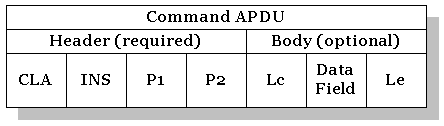
\includegraphics[width=0.7\linewidth]
  {images/section_2/command.png}
\end{subfigure}
\caption{Command Structure [?]}
\end{figure}

% IMAGE: Different Commands
\begin{figure}[H]
\begin{subfigure}{1\textwidth}
  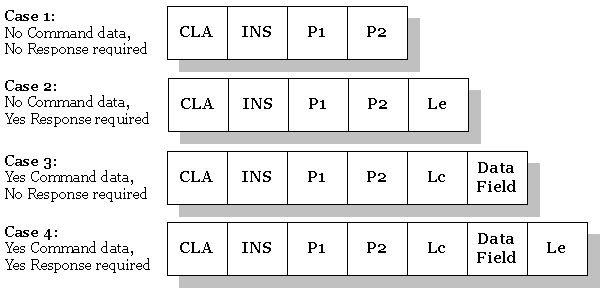
\includegraphics[width=1\linewidth]
  {images/section_2/command_cases.png}
\end{subfigure}
\caption{Different Command Possibilities [?]}
\end{figure}

% Table: Response fields
\begin{table}[H]
\begin{tabular}{|l|p{10cm}|}
\hline
Field & Description\\
\hline
Data & Data is a field that has maximum length 256 bytes. It provides that data the response sends back to the API. \\
\hline
SW1 & SW1 is the first status bytes.\\
\hline
SW2 & SW2 is the second status bytes.\\
\hline
\end{tabular}
\caption{Response Field Explanations}
\end{table}

% IMAGE: Response
\begin{figure}[H]
\hskip+3.5cm\begin{subfigure}{1\textwidth}
  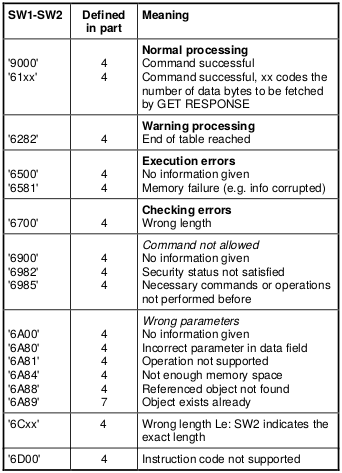
\includegraphics[width=0.5\linewidth]
  {images/section_2/response.png}
\end{subfigure}
\caption{Response Structure [?]}
\end{figure}


ISO/IEC 7816 - section 7 provides the meaning behind the status bytes SW1 and SW2. We have provided a summary of the common types of status bytes and their meanings. This is reported in figure 2.4. Due to the amount of decodings for the status bytes, we only give the exact decoding of them if and when they are required throughout this paper.

% IMAGE: 
\begin{figure}[H]
\centering
\begin{subfigure}{1\textwidth}
  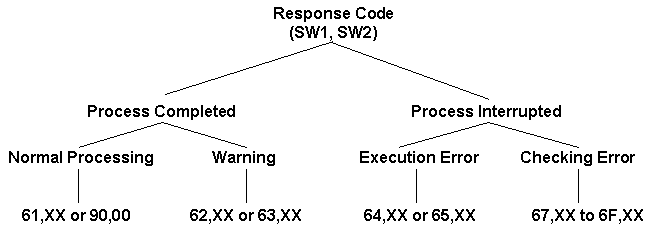
\includegraphics[width=1\linewidth]
  {images/section_2/response_explain.png}
\end{subfigure}
\caption{Response Meanings [?]}
\end{figure}


\subsection{File System}

As defined in section 4 of the ISO/IEC 7816 standard, contact smartcards have a standard for their file systems. A master file (MF) is the root of the file structure, this is analogous to the C drive for windows operating systems on computers. Under the MF are dedicated files (DF) and elementary files (EF). DF's are directories (similar to folders) and have EF's contained within them. EF's are files consisting of data. There are 4 types of files that EF's support, they can be viewed in figure 2.5 and are:
\begin{enumerate}
\item Transparent Binary File
\item Linear structure with records of fixed size
\item Linear structure with records of variable size
\item Cyclic structure with records of fixed size\\\\
\end{enumerate}

Elementary Files (EF) also take on two different formats. These have been witnessed within our analysis in chapter 6. \textit{The explanations of the formats have been taken directly from the standard [?]}:
\begin{enumerate}
\item An internal EF stores data interpreted by the card, i.e., data used by the card for management and
control purposes.
\item A working EF stores data not interpreted by the card, i.e., data used by the outside world exclusively.
\end{enumerate}

% IMAGE: File structure
\begin{figure}[H]
\hskip+0.0cm\begin{subfigure}{0.8\textwidth}
  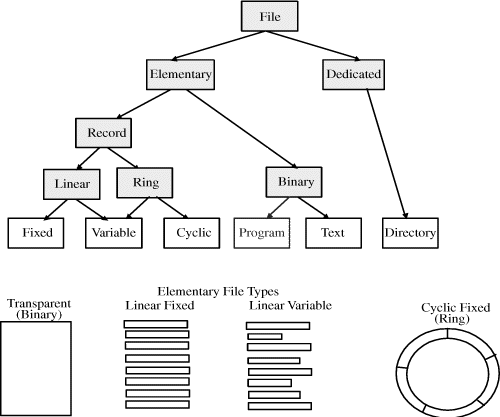
\includegraphics[width=1\linewidth]
  {images/section_2/file_structures.png}\\\\\\
\end{subfigure}
\caption{File Structure [?]}
\end{figure}


\subsection{Secure Messaging}

ISO/IEC 7816 section 4 reports details of the command structure of messages that occur within a 'secure messaging session'. We provide an example of the command structure in table 2.8 (the CLA byte is equal to 8C).

Secure messaging sessions derive two session keys S$_{Enc}$ and S$_{Mac}$ between the API and the smartcard. The S$_{Enc}$ session key is used to encrypt the data-field of commands within a secure messaging session. And S$_{Mac}$ is used to compute a checksum (using C-MAC) of the entire command. This checksum is appended to the command. This provides confidentiality (only the systems in question should be able to read the actual messages) and integrity (data has not been altered in transit) to command-response pairs in a secure messaging session. 

We report the use of secure messaging within chapters 6 and 7.

%---------------------------------------------------------------------------------------------------------------------------------------------------

\chapter{Literature Review}

This will be a brief chapter and will discuss all of the research I have conducted.\\
Mainly regarding PKCS\#11 API attacks due to the small amount of literature that is available for APDU level attacks
I shall also explain why some of the attacks are not able to be conducted on the particular card I am reviewing
\section{RAID (2016)}

\section{REPROVE}

\section{Wrap/Decrypt Attack}
\section{(name) 2015 - Previous study on the same smartcard}
\section{Extended Work}
\subsection{Directories of Key and Attribute Files}
% Table: File locations within Athena IDprotect smartcard
Previous work completed by (name) 2015 [?] had found that attributes and sensitive key values are stored within separate files in the smartcard. It appears that the sensitive key values are stored in internal EF's to prevent extraction, and the attributes are placed in working EF transparent binary files. 

The work also found the location of these attribute files and key value files. However, we extended this work to include the locations of RSA key files. As the previous work only included the directories of block cipher key files (and assumed that asymmetric key value files were stored within the same directory). We discuss this within the literature review in chapter 5, but also list the directory of key and attribute files in table 2.9.

\begin{table}[H]
\hskip+2.0cm\begin{tabular}{|l|l|p{6cm}|}
\hline
Key Type & File Type & Directory\\
\hline
Block cipher & Attribute & 3F 00 30 00 30 \textbf{01 03 4X} \\
 			 & Key       & 3F 00 30 00 30 \textbf{01 00 CX} \\
\hline
RSA public 	 & Attribute & 3F 00 30 00 30 \textbf{02 01 4X} \\
		   	 & Key	     & 3F 00 30 00 30 \textbf{02 00 8X} \\	   	 
\hline
RSA private 	 & Attribute & 3F 00 30 00 30 \textbf{02 01 4X} \\
		   	 & Key	     & 3F 00 30 00 30 \textbf{02 02 0X} \\	   	 
\hline
\end{tabular}
\caption{Directories of Key and Attribute Files}
\end{table}

\subsection{APDU Commands Found During Analysis}

During the analysis of the PKCS \#11 functions and how they are broken down into multiple ISO 7816 command-response pairs for the Athena IDprotect smartcard we analyse in this paper, we found the use of the following inter-industry and proprietary commands.

\textit{[The work from (name) 2015 [?] found the 'inner-function' names which gave a good decoding of the proparitary commands listed in table 2.8. He had utilised a program named 'pcsc-spy' to find the 'inner-function' names. We discuss this within chapter 4 of this paper]}

\begin{table}[H]
\hskip-1.0cm\begin{tabular}{|c|c|c|c|c|c|c|p{8cm}|}
\hline
CLA & INS & P1 & P2 & Lc  & Data Field & Le & Description\\
\hline
00  & -   & -  & -  & -   & -          & -  & Inter-industry (II)\\
80  & -   & -  & -  & -   & -          & -  & Proprietary (P)\\
Xc  & -   & -  & -  & -   & -          & -  & Secure Messaging (SM)\\
\hline
00  & 84  & 00 & 00 & -   & -          & L  &  (II) Get Challenge [\# bytes = L]\\
00  & B0  & X  & X  & -   & -          & L  &  (II) Read Binary [\# bytes = L] \\
00  & C0  & 00 & 00 & -   & -          & L  &  (II) Get Remaining Bytes\\
00  & D6  & X  & X  & L   & X          & -  &  (II) Update Binary\\
00  & E0  & X  & X  & L   & X          & -  &  (II) Create Binary\\
00  & 47  & 00 & 00 & L   & Params     & -  &  (II) Generate RSA KeyPair\\
00  & E4  & 00 & 00 & 00  & -          & -  &  (II) Delete File\\
00  & 2A  & 82 & 05 & L   & X          & 00 &  (II) Encrypt Data \\
00  & 2A  & 80 & 05 & L   & X          & 00 &  (II) Decrypt Data \\
00  & 2A  & 9E & 12 & L   & X          & 00 &  (II) Sign Data \\
00  & 2A  & 80 & 0A & L   & X          & 00  & (II) Unwrap Key (RSA\_PKCS)\\
\hline
80  & A4  & 08 & 00 & L   & FL         & -  & (P) Select File [FL = file location; L = len(fl)]\\
80  & A4  & 00 & 00 & -   & FL         & -  & (P) Select File [append previous path]\\
80  & A4  & 08 & 0C & L   & FL         & -  & (P) Read File Control Parameters\\
80  & 20  & 00 & 00 & 10  & R          & -  & (P) Verify PIN [R = Response]\\
80  & 28  & 00 & 00 & 04  & 00 00 00 20& -  & (P) Clear Security Status\\
80  & 30  & 01 & 00 & 00  & -          & -  & (P) List Files\\
80  & 48  & 00 & 80 & 00  & -          & -  & (P) Get The Smartcards Public Key [SM]\\
80  & 48  & 00 & 00 & 00  & -          & -  & (P) Get Generated Public Key\\
80  & 86  & 00 & 00 & L   & X          & 00 & (P) Open Secure Messaging\\
80  & 86  & FF & FF & -   & -          & -  & (P) Close Secure Messaging\\
\hline
90  & 32  & 00 & 03 & ff  & X          & -  &  Reallocate Binary 256 bytes\\
80  & 32  & 00 & 03 & L   & X          & -  &  Reallocate Binary L bytes (changes file)\\
\hline
\end{tabular}
\caption{Common APDU Commands}
\end{table} 


\subsection{Manually Overriding Attributes}
This attack was found by previous literature. We simply tested to see if the same attack was feasiable on the smart card we analyse. 

To test this we created a DES3 key on the card that had the encrypt attribute set to False. We asked the card to encrypt the string '12345678'. The API returned an error stating that this function was not supported due to the attribute settings. We then override the API by manually sending the command overselves. This results in the encryption taking place on the card, when in-fact it should not.

%---------------------------------------------------------------------------------------------------------------------------------------------------


\chapter{Tools Developed/Used In This Project}



\section{PCSC-lite}

\section{Virtual Smartcard}
frank something
Explain how this creates a virtual smartcard reader
This is then used to run API functions, and the commands are relayed to the actual card reader and therefore card.


\section{Man in The Middle (MiTM)}



%---------------------------------------------------------------------------------------------------------------------------------------------------

\chapter{PKCS \#11 Functions - APDU analysis}

As discussed in chapter 2, PKCS \#11 API functions are broken down into multiple ISO 7816 command-response pairs via the use of the card vendors middleware \textit{(their implementation of the PKCS \#11 API)}. This implementation is  at the manufacturer's discretion, who may wish to use proprietary commands. The aim of this chapter is to analyse the APDU traces of 9 PKCS \#11 functions, and how the card manufacturer has decided to split them into command-response pairs. 

This is because previous literature has shown that some poor implemenations has revealed PIN's and encryption keys at the APDU layer which heavily violate the PKCS \#11 standard. Our analysis will include a step by step guide as to how the functions are broken down into command response pairs at the APDU level.  In addition, the analysis will provide explanations of how the implementation operates and therefore be able to suggest possible vulnerabilities, some of which will be investigated in chapter 7. 

All the traces are reported in appendix B. These traces have been shortened to only include the command-response pairs which are deemed to be the most important to the evaluation of a function. However, the full traces for each function are given within the project directory. We will refer to appendix B including the corresponding command response pair which are given in brackets to allow ease of locating the steps throughout our analysis.

\textit{C\_sign} and \textit{C\_verify} are not included in this analysis as earlier work [?] on this card show that both of these functions operate in a similar manner to C\_encrypt and C\_decrypt. \textit{C\_createObject} is also not included in this analysis, because it operates in a similar fashion to \textit{C\_generateKey} and \textit{C\_generateKeyPair}. The only difference is that the key values are provided by the user rather than being computer generated.

To prevent repetition we list the dependencies (other functions that must be run before hand) at the start of each section when necessary.

It is worth stressing that chapter 6 will only provide explanations of the possible vulnerabilities that might be present. We leave all the investigations of them to chapter 7.


\section{Initialization}

Initialization is process whereby the smart-card sends 2 serial numbers to the API, in order for the API to have the knowledge of which model of smartcard it is to communicate with. This occurs as soon as a session is opened with the card. The process has the following steps:
\begin{enumerate}
\item Open the laser PKI file and select the applet (B.1 - command 1)
\item Send to the API the card serial number (B.1 - command 4,5)
\item Send to the API the 2nd serial number (B.1 - command 8,9)
\end{enumerate}

The trace doesn't reveal sensitive information. These steps are required in order for the card to operate and communicate with the API. The API is a generic library that works with many different hardware security modules created by the 'Athena smartcard solutions'. Hence the serial numbers are required by the library in order for it to operate correctly for the specific type of card.

\section{C\_login}

\textit{Function dependencies $\rightarrow$ [Initialization]}\\


The login function has 5 main components (these are listed below). 

\begin{enumerate}
\item Open file control parameters for file X$_1$ (B.2 - command 10)
\item Select file X$_2$ (B.2 command 11)
\item Request challenge from the card (B.2 - command 12)
\item Use the proprietary VERIFY command for verification of PIN value (B.2 - command 13)
\item Clear security Status (B.2 - command 20)\\
\end{enumerate}

The API requests to view the file control parameters for file X$_1$. The file location as stated within the trace is at '3F 00 00  20 00'. This holds the retry counter value, which dictates how many attempts are left before the card is blocked \textit{(A value of 'A0' states the card is currently in a blocked status)}. To make it easier to locate within the trace we have highlighted the current value in bold which is of 'AA', meaning there is 10 attempts left.

Following this check, file X$_2$ is selected. We assume that this file holds a pointer to EEPROM memory where the PIN is securely stored by the smartcard. This file cannot be accessed with the inter-industry command 'READ BINARY' nor the proprietary command 'READ FILE CONTROL PARAMETERS'. However if this file is not selected PIN verification fails despite having the correct PIN value. This finding was reported by (enter name) last year [?].

After file X$_2$ has been selected, the API requests the smartcard to send an 8 byte challenge. Upon receiving said challenge, the API then responds with a 16 bytes of data for PIN verification using the proprietary 'VERIFY' command. Assuming the correct PIN has been supplied the user is now authenticated with the card, and the last step clears the security status.

The evaluation of multiple traces of the login function shows that the response calculated appears to have an element of randomness. From studying the traces alone, the method of calculating the value of the response, given the PIN and the smartcards challenge, cannot be intuitively determined.

No immediate sensitive information is revealed in this trace, due to the use of the challenge-response algorithm used for verifying a user's PIN. However, if an attacker can successfully reverse engineer the challenge-response protocol, the PIN can be calculated given 1 successful login trace. Furthermore, if an attacker can find a method for changing the file control parameters, they might be able to reset the retry counter at the APDU level to allow an unlimited number of attempts of logging in. These possible vulnerabilities will be discussed in detail in chapter 7.

\section{C\_findObject}
\textit{[For this trace to show meaningful information we have generated and stored a triple DES key onto the card, before running the findObject function. The label of the key was 'des3' with id '01']}

\textit{Function dependencies $\rightarrow$ [Initialization, Login]}\\


The findObjects function is split into 3 main components (these are listed below).

\begin{enumerate}
\item Select and open 'cmapfile' [List files command]. This stores all file locations for attributes of the keys (B.3 - command 32, 33, 34)
\item Using the data from 'cmapfile', Open the first attribute key file (B.3 - command 36)
\item Open the next attribute key file. (Which is empty) (B.3 - command 38, 39)\\
\end{enumerate}


First, a cmapfile is accessed. This file stores the location of key attribute files. Following this, attribute files are accessed. The attribute files store all the information regarding a specific keys attributes (listed in section 2.1.2). Finally the next (and last) file is opened. In the case more than one key was stored on the card at the time of running this function the next file would contain the attributes of the next key. However, since there is only 1 key, the next file is empty (containing all zero's) thus determining there are no more key objects to be found.

Due to key and attribute files being stored separately, this function call reveals no sensitive information. This finding was reported by (name) 2015 [?] and is stated within our literature review. Only the attributes are opened and listed at the APDU layer. These attributes can be printed at the API layer as well.

A possibility for an attack is present here. The ISO 7816 proprietary 'REALLOCATE BINARY' and the inter-industry 'UPDATE BINARY' commands can be used to modify a file. This will allow modification of attributes. 

As reported in the literature review, the work by (name) 2015 [?] on the same card shows that they were able to modify any attributes. They tested the modification of CKA\_sensitive \& CKA\_extractable from false to true. The change in this direction is not permitted by the PKCS \#11 standard. However the ability to change these at the APDU level was achieved. This approach still yielded no significant results, as keys and attribute are stored in separate files, thus the keys could still not be loaded. This is discussed in chapter 7.

\section{C\_generateKey}
\textit{[For this trace we generate a triple DES key, key length of 24 bytes.]}

\textit{Function dependencies $\rightarrow$ [Initialization, Login]}\\

The generateKey function has 9 main components (these are listed below).

\begin{enumerate}
\item Open secure messaging (B.4 - commands 26, 27, 28)
\item Generate 24 random bytes and send them to the API via secure messaging (B.4 - command 29)
\item Close secure messaging (B.4 - command 30)
\item commands skipped include finding spare file for attributes and opening the file.
\item Update file with key attributes (B.4 - commands 40, 41)
\item Open secure messaging [again] (B.4 - commands 42, 43, 44)
\item Open key file directory via secure messaging (B.4 - command 45)
\item Create key file for triple DES key via secure messaging (B.4 - command 46)
\item Close secure messaging (B.4 - command 47)\\
\end{enumerate}

Secure messaging session have an initialization process whereby the API and smartcard generate 2 session keys S$_{Enc}$ and S$_{Mac}$. Once the initialization is completed the following communications data fields are encrypted with S$_{Enc}$ and a checksum is computed via C-MAC (see section 3.4.2) using S$_{Mac}$. They provide confidentiality and integrity of the data being sent within the data fields of the commands during a secure messaging session.

Two different secure messaging sessions are used. The first is to request the card to generate 24 bytes (same as the key length) and send it to the API. The second is to place the key value into the key file. The attribute file is created without the use of secure messaging as it does not contain sensitive information.

The analysis of the communication trace suggests that the card is requested to generate the key value from a 'GET CHALLENGE' request (within secure messaging). We assume that the generated bytes are used to be stored in the key file as the key value. At this stage it is not possible to verify this. The reason being that two different secure messaging sessions are used, and therefore have different session keys. This causes the encryption of the generated bytes and the storing of them in a file, to be different. Despite the possibility they might be identical. 

As discussed in the literature review chapter, previous hardware security modules created by 'Athena smartcard solutions' have in the past requested the card to generate random bytes and use them as the key value (when generateKey function is called). This was completed without the use of secure messaging. Thus, it appears that they might be using a similar approach but with the use of secure messaging (to prevent revealing the encryption keys in plain text at the APDU layer) on this smartcard.

If the assumption of the generated bytes being used as the key value holds, it may result in a significant vulnerability that could be exploited. This will only be valid if the secure messaging protocol (that is a proprietary implementation by the card vendor) can be reversed engineered. This should allow an attacker to inject a new key value or decrypt the key value to be stored. This would be in breach of the PKCS \#11 standard, depending on attribute values set.

A second vulnerability is also present. Unlike previous attacks whereby attributes are modified after a key has been created. An attacker could modify the attributes during the key generation process (this would take place at step 5, in the component list above). Changing attribute values would allow for the key to be extracted as soon as it is created (this has been checked). It is worth noting that the user will be aware of it, as it is printed at the API layer. In addition they will also be able to see the modified attributes which they had not set. Thus we determine this to be a vulnerability, but not as serious as the previous one mentioned. As if it were utilised, the user would most likely notice and therefore generate a new key to be used.

Both of these possible vulnerabilities are discussed in chapter 7.



\section{C\_generateKeyPair}
\textit{[For this trace we generate an RSA-1024 public/private key pair]}

\textit{Function dependencies $\rightarrow$ [Initialization, Login]}\\

We find 15 main components in this generation of the RSA public and private key pair (these are listed below).

\begin{enumerate}
\item Create public key attribute file (B.5 - command 54)
\item Add public key attributes to file [inc. public exponent] (B.5 - commands 56, 57)
\item Create private key attribute file (B.5 - command 59)
\item Add private key attributes to file (B.5 - commands 61, 62)
\item Create Private CTR RSA Key file (B.5 - command 64) [ref crypto section] [?]
\item Select temporary file (B.5 - command 65)
\item Generate RSA Key Pair (B.5 - command 66)
\item Select temporary file (B.5 - command 67)
\item Get RSA public key (B.5 - command 68)
\item Select parent folder of private key attribute file (B.5 - command 69)
\item Create new file, with public modulus and additional info (B.5 - command 70
\item Select temporary file (B.5 - command 71)
\item Get RSA public key (B.5 - command 72)
\item Select public attribute file (B.5 - command 73)
\item Add public modulus to attribute file (B.5 - command 74)\\\\
\end{enumerate}

\textit{The rest of the communication we believe to be resetting the temporary file, and adding file location information to file control parameters of parent directories. (These commands are not included in the traces within the appendix)}

Components 1, 3, 5, 7, 9, 11, and 13 transfer data that are wrapped within an ASN.1 BER encoding [?]. We have used an online tool [?] to decode the data fields. The following are the ASN.1 BER decodings of the commands that have these wrapping. 

\textbf{1. Create public key attribute file (B.5 - command 54)}\\
Application 2(4 elem)\\
$[10]$ (1 byte) 04\\
$[03]$ (2 byte) \textbf{01 40}\\
$[00]$ (2 byte) 01 A7\\
$[06]$ (8 byte) 00 20 00 20 00 20 00 20\\

\textbf{3. Create private key attribute file (B.5 - command 59)}\\
Application 2(5 elem)\\
$[10]$ (1 byte) 04\\
$[03]$ (2 byte) \textbf{02 00}\\
$[00]$ (2 byte) 01 23\\
$[04]$ kx s0\\
$[06]$ (8 byte) 00 00 00 20 00 20 00 20\\

\textbf{5. Create private CTR RSA key file (B.5 - command 64)}\\
Application 2(6 elem)\\
$[10]$ (1 byte) 04\\
$[03]$ (2 byte) \textbf{00 41}\\
$[00]$ (2 byte) 00 80\\
$[05]$ (5 byte) 05 0C 20 00 A3\\
$[06]$ (14 byte) 00 00 00 FF 00 FF 00 20 00 20 00 00 00 20\\
Application 17(0 elem)\\

\textbf{7. Generate RSA key pair (B.5 - command 66)}\\
$[12]$ (2 elem)\\
$[00]$ (1 byte) 06\\
$[01]$ (3 byte) 01 00 01\\

\textbf{9,13. Get RSA public key (B.5 - commands 68, 72)}\\
Application 73(2 elem)\\
$[01]$ (128 byte) D1 EF 7C A5 06 A1 87 FD 5F 13 5B 25 B7 16..\\
$[02]$ (3 byte) 01 00 01\\

\textbf{11. Create new file with public modulus and additional info (B.5 - command 70)}\\
Application 2(6 elem)\\
$[10]$ (1 byte) 04\\
$[03]$ (2 byte) \textbf{00 81}\\
$[00]$ (2 byte) 00 80\\
$[05]$ (5 byte) 05 08 20 00 A3\\
$[06]$ (14 byte) 00 00 00 FF 00 FF 00 20 00 20 00 00 00 20\\
Application 17(2 elem)\\
$[16]$ (3 byte) 01 00 01\\
$[17]$ (128 byte) D1 EF 7C A5 06 A1 87 FD 5F 13 5B 25 B7...\\

RSA key pair generation occurs on the card. A dedicated processor is used for this, hence the need to change to temporary files to access the generated key and then store the public information. We notice no sensitive information being revealed within the traces in plain text. We are of the opinion that the information provided that is wrapped within the ASN.1 BER encoding, especially for \textbf{5}, might have exported the private key and the additional parameters required for CRT RSA keys [?]. To test this theory we have deleted the generated key and generated another RSA key. This resulted in the public modulus of the RSA key to change, but the remaining parameters did not. A change in the public modulus would cause a change in both the private exponent and CRT parameters. This leads us to conclude that no part of the private key is exported in plain text within the communication traces.

As we will explain in the destroyObject function analysis, when a key is deleted from the card, the location in memory where the keys are securely stored (i.e. cannot be read) is revealed. We have used the destroyObject function to delete both RSA public and private keys. This enabled us to find the locations of the key and attribute files for both keys. These results are reported below:

\begin{table}[H]
\begin{tabular}{|l|c|c|}
\hline
 & Key File & Attribute File\\
\hline
RSA public key & 3F0030003002 \textbf{00 81} (11. [03]) & 3F0030003002 \textbf{01 40} (1. [03])\\
\hline
RSA private key & 3F0030003002 \textbf{02 00} (3. [03]) & 3F0030003002 \textbf{00 41} (5. [03])\\
\hline
\end{tabular}
\caption{File Location Table}
\end{table}

Our work shows that components 1, 3, 5, and 11 (listed above) are used to save the details of the location in the smartcard's memory of the RSA public \& private attribute and key files. The corresponding componenets with the file location parameters are reported in brackets in the table 6.1. Components 9 and 13 reveal the RSA public exponent and modulus used to be saved into attribute and key files. Finally, component 7 is used to give the size of the RSA key and its public exponent for key pair generation on the card.

Therefore, the only vulnerabilities we notice are, the ability to modify attributes as the key is being generated (components 2 and 4). This was discussed within generateKey function analysis and did not prove to be a vulnerability that would not be noticed by the user. The second vulnerability is the disclosure of the file location of the private key. The opening and possible reading of the key value is discussed as part of the destroyObject function analysis and also in chapter 7.

\section{C\_destroyObject}
\textit{[For this trace we delete/destroy a triple DES (key option 2) 16 byte key and its attribute file]}

\textit{Function dependencies $\rightarrow$ [Initialization, Login, FindObjects]}\\

Once the key and attribute files have been located and the user is authenticated with the card, there are 6 main components to the destruction of the object. These are listed below:\\

\begin{enumerate}
\item Select counter file for key attributes (B.6 - command 49)
\item Update counter (B.6 - command 50)
\item Select key file (B.6 - command 53)
\item Delete key file (B.6 - command 54)
\item Select key attribute file (B.6 - command 55)
\item Delete key attribute file (B.6 - command 56)
\end{enumerate}

Work conducted by (name) 2015 [?] did show that the counter file maintains track of how many keys have been created and deleted in a certain path within the smartcard's memory. We are unsure about its specific use (except for maintaining track of the number of keys) as we have only seen it being updated upon deletion of an object, and the new counter value being appended to the new keys attributes (the one created after deleting an object). The original and updated counter value is reported in appendix B.6 - command 37 and 50 respectively.

Once the counter file has been updated, the key attribute file and the key file are selected and deleted using the inter-industry command 'DELETE FILE'. This is the first finding where the location of a key file  is accessed without the use of secure messaging. The finding is consistent with the earlier work [?]. Thus we think that this may present a vulnerability which would allow us to open and read key values at the APDU level. 

We attempt to use the 'SELECT FILE' command and then 'READ BINARY' command to try and read the files data. This resulted in an error message = '69 81', meaning the command is incompatible with the file structure. In out next step, we try the other command which is 'OPEN FILE CONTROL PARAMETERS'. This did successfully work. We find that the output is wrapped in an ASN.1 BER encoding, thus we decoded it this gave the following result:

Application 2(6 elem)\\
$[07]$ (1 byte) 08\\
$[03]$ (2 byte) \textbf{00 C1}\\
$[00]$ (2 byte) 00 18\\
$[10]$ (1 byte) 04\\
$[06]$ (14 byte) 00 00 00 FF 00 FF 00 00 00 00 00 00 00 00\\
$[05]$ (4 byte) 01 0C 10 00\\

The above decoding is similar to what we have reported for the RSA private key analysis in section 6.5. The 16 byte key that would be used for triple DES is not present. There is however pointers to the file that we just read the parameters of \textit{(00 C1)}, and other additional parameters that we are unsure of their use. 

All security policies [?] that we have reviewed concerning 'Athena smartcard solutions' suggest that keys are stored in internal EF's (cannot be accessed by outside actors, see section 3.2.1, chapter 3), and only when required are encrypted internally (by the smartcard's OS) and stored in the EEPROM (electrically erasable programmable read only memory) for them to be used for the security operation required of them. 

Thus we did not find any security vulnerabilities from this function. And also eliminates one of the vulnerabilities we suggested within the generateKeyPair function analysis. We discuss further in chapter 7.

\section{C\_encrypt}
\textit{[For this function we use a triple DES key to encrypt a string 'TestString123456'] using ECB mode]}

\textit{Function dependencies $\rightarrow$ [Initialization, Login, FindObjects]}\\

The commands given for this trace are actually repeated and therefore occur twice for one encrpytion of a given string. This is due to PKCS \#11 library being programmed in C by the card's manufacturer. The resulting length of the encryption is assumed to be of an undetermined size (for block ciphers and even RSA this can be pre-calculated given the input length). However the implementation runs the encryption twice, the first run is to calculate the resulting length of the encryption, and the second run saves the result in a buffer that has been pre-allocated the correct number of bytes in a char array.

This function only has only 2 main components (these are listed below).\\

\begin{enumerate}
\item Select key file (B.7 - command 52)
\item Encrypt data (B.7 - command 53)\\
\end{enumerate}

The key file is selected and then the encryption APDU command is called with the string in the data field. As explained in destroyObject function analysis, despite the key file location being revealed here, it does not present a vulnerability. The key file can neither be opened nor reveal the value of the key. Instead it provides pointers to other locations in the smartcard's memory that hold the key value securely. It is reasonable to assume (though unable to test or verify) that only the smartcard's operating system has access to these locations.

Therefore we find no evidence of other vulnerabilities that can be exploited.

\section{C\_decrypt}
\textit{[For this trace we use the same triple DES key to decrypt the message we previously encrypted]}

\textit{Function dependencies $\rightarrow$ [Initialization, Login, FindObjects]}\\

The decrypt function operates nearly in an identical manner to the encrypt function. The only difference is that it simply changes one byte (P1 in the APDU command header) in command 65. The key is loaded and then the decrypt APDU command is sent, with the encrypted string placed in the data field. For the same reasons stated in the encrypt function, the APDU command is sent twice. 

It also has 2 main components (these are listed below).\\

\begin{enumerate}
\item Select key file (B.8 - command 64)
\item Decrypt data (B.8 - command 65)\\
\end{enumerate}

As the decrypt function operates in a similar fashion to the encrypt function, we find no vulnerabilities here either. However we did find a similar implementation flaw that has been reported in earlier work [?] regarding decryption using an AES block cipher key in ECB mode. For an unknown reason the first 8 bytes are removed from the encrypted data. This only decrypts and returns the second 8 bytes. As this does not present a security vulnerability, but it is rather an issue with the functionality of the decrypt function. Therefore for this reason we do not analyse it any further.

\section{C\_setAttribute}
\textit{[For this trace we modify the label of the triple DES key from 'des3' to 'changed']}

\textit{Function dependencies $\rightarrow$ [Initialization, Login, FindObjects]}\\

Similar to encrypt and decrypt, this function has only 2 main components. The first one selects the attribute file, and the following 2 commands update the whole file to include the new name of the label to the key. The components are listed below:\\

\begin{enumerate}
\item Select key attribute file (B.9 - command 51)
\item Modify attribute file to change the label name from 'des3' to  'changed' (B.9 - commands 52,53)\\
\end{enumerate}

Command chaining (see section 2.2) was used as the number of bytes within the attribute file exceeded the limit of 256. Command chaining is indicated by the use of '90' instead of '80' as the CLA byte. This was seen in the 'REALLOCATE BINARY' command that was used to modify the attribute file.

We notice that at the APDU layer attributes can be changed  via the 'REALLOCATE BINARY' command. This is a vulnerability that was discovered and tested in previous work [?]. With the main focus on changing the attribute values of CKA\_sensitive and CKA\_extractable from true to false and false to true respectively. The change in this direction is not permitted by the PKCS \#11 standard. However, this was conducted at the APDU layer. The tests carried out in the literature found that due to the split between attribute files and key value files, the key value could still not be extracted despite the modification to the attributes.

Thus, despite the vulnerability being present it does not appear to cause a major security issue, in the sense that the key value is still stored securely. We discuss this further in chapter 7.


\section{C\_unwrap}
\textit{[For this trace we used an RSA public key to encrypt a triple DES key value = 12345678. With its encryption saved, we then create a template for the key attributes and used the RSA private key to unwrap the key value and template, to save the key on the card]}

\textit{Function dependencies $\rightarrow$ [Initialization, Login, FindObjects, Encrypt]}\\


There are 10 main components involved in the unwrapping of a key. 2 different secure messaging sessions are used (just like in the generateKey function). The first secure messaging session is used to unwrap the encrypted key into a temporary file. The second secure messaging session is used to save the triple DES key into a key file. This follows after the attribute file has been created in between these 2 secure messaging sessions. The order of the components are listed below:\\

\begin{enumerate}
\item Open secure messaging (B.10 - command 92, 93, 94)
\item Select a file [the file location is encrypted and therefore unknown] (B.10 - command 95)
\item Unwrap key and attributes (B.10 - command 96)
\item Close secure messaging (B.10 - command 97)
\item Select key attribute file (B.10 - command 119)
\item Add key attributes to file (B.10 - command 120, 121)
\item Open secure messaging (B.10 - command 122, 123, 124)
\item Select the key file directory (B.10 - command 125)
\item Create key file (B.10 - command 126)
\item Close secure messaging (B.10 - command 127)\\
\end{enumerate}

In a scenario where we are not already in the knowledge of the key value, the secure messaging sessions are the main vulnerability that we will aim to try and exploit. While the key is not exported at the APDU layer in plain text. Successfully reverse engineering the secure messaging protocol, would allow an attacker to exploit it. This can be achieved by injecting our own session keys and decrypt the key value. This was discussed in analysis of the generateKey function.


Furthermore, an attacker can also modify the attributes as the key is saved within the card for the first time. But as discussed in the generatKey function analysis, this attack would make the user aware of the fact that the key has been exported and the attributes have been changed. This cannot be deemed as serious a vulnerability compared to one that would expose the key in plain text at the APDU layer without the user's knowledge. These possible vulnerabilities are discussed further in chapter 7.


\section{C\_wrap}
As discussed in section [?] of the literature, the wrap/decrypt attack is carried out at the API level whereby one key can be given wrapping and decryption functionalities within its attributes. This allows for any key (regardless of the attributes) to be wrapped, exported out of the card, and then decrypted by the same key. This would reveal its key value in plain text. This vulnerability bypassed all controls that the attributes of a key are expected to provide. Due to this vulnerability discovery, it is reasonable to assume that 'Athena smartcard solutions' decided to remove the ability to wrap keys completely in an attempt to prevent this type of attack. This reasoning is based on the fact that requesting any key to wrap another key at the API level causes an error: \textit{CKR\_Function\_Not\_Supported}.

From the analysis of table 2.1 (see section 2.2.4), we find a correlation between the P1 and P2 parameters for the APDU commands for encryption, decryption and unwrapping. These values are tabulated below:

\begin{table}[H]
\begin{tabular}{|c|c|l|}
\hline
P1 & P2 & Command\\
\hline
82 & 05 & encrypt\\
80 & 05 & decrypt\\
80 & 0A & unwrap\\
? & ? & wrap\\
\hline
\end{tabular}
\end{table}

\textit{The CLA and INS bytes are identical for all of the above commands.} 

Given the fact that for encrypt and decrypt, P2 remains the same and only P1 alters from '82' to '80', we infer that if the wrap command still exists at the APDU layer, then the values for P1 and P2 would be \textbf{82} and \textbf{0A} respectively. Therefore, an example full command would be: \textbf{00 2a 82 0a L Data 00}. Were L is the length of the data, and the data is the key to be wrapped. 

We ran a simple test to see if this command operates on the card:
\begin{enumerate}
\item Wrap key (string '12345678') (B.11 - command 1)\\
\end{enumerate}


The result of the test shows an error at the APDU level. The error value was '6A 80', meaning the parameters within the data field are incorrect. This suggests that the command does exist and most likely corresponds to the wrap function.

The data field of unwrap is encrypted, as it is used within secure messaging. However if this was reversed engineered and we are able to understand the data field of the unwrap command, it will be highly likely that we would be able to create the correct data field for the wrap command. This would allow us to bypass all attribute controls of keys at the API level, and implement the wrap/decrypt attack at the APDU level. This in turn would allow all keys on the card to be exported out of the card in plain text. This would be a serious violation of the PKCS \#11 standard.





%---------------------------------------------------------------------------------------------------------------------------------------------------


\chapter{New Attack's At the APDU Level}

In this chapter we explain the motivations, implementation and results of the attacks we attempt as the APDU level. For clarity purposes we first give a brief overview of the API's function analysis at the APDU layer that we conducted within chapter 6. This analysis in combination with previous work completed on the same smartcard and for that matter other smartcards as well, drove the motivations behind the attacks we selected to conduct.

\section{Motivations}
\begin{table}[H]
\hskip-1.5cm\begin{tabular}{|p{7cm}|p{4cm}|c|}
\hline
Vulnerability & Functions & To be Investigated Further\\
\hline
Modifying attributes (keys already generated) & C\_findObjects & $\chi$ \\
\hline
Modifying attributes (as keys are being generated) & C\_generateKey, C\_generateKeyPair & $\chi$\\
\hline
Opening key file memory locations & C\_encrypt, C\_decrypt, C\_generateKeyPair, C\_destroyObject & $\chi$\\
\hline
Reverse engineering PIN authentication protocol & C\_Login & \checked\\
\hline
Reverse engineering secure messaging protocol & C\_generateKey, C\_unwrap & \checked\\
\hline
Wrap/Decrypt attack at the APDU layer & - & future work\\
\hline
Modifying the retry counter & C\_login & future work\\
\hline
\end{tabular}
\end{table}
\subsection{Vulnerabilities not investigated}
The \textit{initialization} function does not reveal any vulnerabilities that cane be exploited and is there for the API to correctly operate.

We have highlighted in the \textit{Login} function analysis that it might be possible to use either 'REALLOCATE BINARY' or 'DELETE FILE' and 'CREATE FILE' in order to modify the retry counter. The aim of this would be to allow an unlimited number of attempts at guessing the user's PIN. We argue that is it not advisable to focus on this attack as it would not be particularly useful without the knowledge of the challenge-response algorithm that is used to verify the user's PIN. Thus, we decided to focus on the reverse engineering of the PIN authentication protocol first, and left this attack for future work.

The vulnerability discussed in the \textit{FindObject} function analysis presents the possibility to locate the attribute files at the APDU level, and modify them using 'REALLOCATE BINARY'. The two attributes that have the most significance would be CKA\_extractable and CKA\_sensitive. Previous work [?] has analysed this vulnerability and the findings did not reveal any significant security concerns. This was due to the fact that once the attributes had been set as part of the key generation process, the attribute file and the key file are separated and thus prevent the key from being exposed in plain text. Since this attack had already been investigated we did not feel that it would be appropriate to investigate it any further at this stage.

\textit{GenerateKey} and \textit{GenerateKeyPair} function analysis both suggest a vulnerability whereby attributes can be modified as the attribute file is being created for the first time. This leaves the possibility of the key value being exposed at the API layer. This effectively could result in the card being instructed to generate the key with the attributes the attacker sets. Setting the key attributes to have CKA\_sensitive set to false and CKA\_extractable set to true, will allow for key value exposure at the API level. This vulnerability would always have to be exploited upon key generation and would be visible to the user of the smartcard. Although this might be a viable attack to investigate, we have decided that it would be better to look into methods that would allow all keys to be exported in plain text regardless of whether the key was already generated and saved on the card without informing the user.

\textit{Encrypt, Decrypt, GenerateKeyPair} and \textit{DestroyObject} functions export in plain text the directory of the key file. Following our discussion in chapter 6, (destroyObject analysis, section 6.6) we hypothesise that this might have provided the ability to open the file and read the key value in plain text. This hypothesis turned out not to be valid, and instead the  we could only view the file control parameters, which stored data wrapped in an ASN.1 BER encoding, that had pointers to locations within the smartcard's memory where the key values are stored securely within internal EF's (see section 3.2.1, chapter 3).

We find that \textit{Unwrap} function does not reveal any vulnerabilities. Instead we would like to learn exactly how the data field is built, but this cannot be inferred from traces as the command is only ever used within secure messaging. Therefore, the data field is encrypted. The rational for focusing on understanding of how the command works is related to possibility of implementing the wrap/decrypt attack at the APDU layer. This is explained in the next section.

\subsection{Vulnerabilities to investigate}

From studying the traces for the \textbf{\textit{login}} function it was apparent that a challenge-response algorithm has been implemented. This helps to provide a secure method for transporting the PIN for verification by the smartcard without ever revealing its value in plain text (which would be in breach of the PKCS \#11 standard). This is an improvement upon implementations from other card manufacturers whereby they did just send the PIN in plain text over the APDU layer for it to be verified. This leaves the possibility of an an attacker simply intercept the communication and extract the user's PIN number. However, the challenge-response algorithm that 'Athena smartcard solutions' has implemented on this card still leaves the potential for an attacker to reverse engineer the protocol, and then brute force the PIN until the same response is calculated to be sent to the card. Doing this would give the attacker the knowledge of the users PIN and also remove the first dependency on the use of the API by an attacker. This is therefore the first attack that we investigate.

Furthermore the use of secure messaging to encrypt and also provide an integrity check (that the commands have not been altered in transit) in the form a message authentication code being appended to the command was found within two functions. These are \textbf{\textit{generateKey}} and \textbf{\textit{unwrap}}. The ability to successfully reverse engineering the secure messaging protocol would allow us to achieve two objectives. First, within the generateKey function an attacker would be able to implement a man in the middle attack to either alter the key being generated with a value known to the attacker, or simply decrypt the key to find out its value. This would be possible regardless of the attributes set for the key, and therefore would violate the PKCS \#11 standard, especially if the attributes for CKA\_sensitive and CKA\_extractable were set to true and false respectively. As an attacker would be able to know the block cipher keys generated when in fact the only system that should be in possession of said knowledge is the smartcard.

Secondly is the understanding behind how the \textbf{\textit{Unwrap}} APDU command operates. As stated in section 6.11, despite the API removing the ability to use the \textbf{\textit{Wrap}} functionality (most likely due the wrap/decrypt attack discovery [?]), with a high probability the APDU command still exists as we managed to send what we believe to be the correct command and received back an error stating the data field parameters were incorrect. Therefore reverse engineering the secure messaging protocol would allow us to fully understand the \textbf{\textit{Unwrap}} command data field, and possibly then be able to generate the correct command for wrapping a key. If this is possible, then the wrap/decrypt attack could be implemented at the APDU level, bypassing all attribute controls and exporting any/ all keys that are stored within the card. This would be considered a serious vulnerability.

All of the vulnerabilities discussed within this section are to be implemented at the APDU layer and would not provide the user the knowledge that an attack is taking place. This is the main reasoning behind selecting these vulnerabilities for further investigation, and the fact they are far more serious compared to the vulnerabilities discussed earlier, in terms of violations of the PKCS \#11 API. Furthermore the attacks suggested for further investigation also remove the dependencies on the use of the API, which will allow an attacker to send commands at the APDU layer independently. This gives an attacker a higher capability.

\section{Reverse Engineering PIN Authentication Protocol}
The first attack we investigate is the reverse engineering of the PIN authentication protocol. If this is successful, an attacker will be able to brute force and/ or use a dictionary attack to calculate the users PIN. The attack shall also remove one dependency on the use of the API. At this stage the API is required to login into the smartcard as we are unaware of how the challenge-response algorithm is implemented. Figure 7.1 shows the procedure for logging into the smartcard at the APDU level.

% IMAGE: challenge-response pin authentication
\begin{figure}[H]
\centering
\begin{subfigure}{1\textwidth}
  \includegraphics[width=1\linewidth]
  {images/section_7/7.2/authencation_method.png}
\end{subfigure}
\caption{Challenge Response Procedures}
\end{figure}

The API requests (via a 'GET CHALLENGE' command) the smartcard to generate and send back 8 random bytes. Based upon the knowledge of the challenge (8 random bytes) and the user's PIN, the API then calculates the 16 byte response. The 16 byte response is sent to the smartcard (via a 'VERIFY' command), which returns one of two possible outcomes:
\begin{enumerate}
\item '90 00' $\rightarrow$ Verification of user's PIN succeeded
\item '63 CX' $\rightarrow$ Verification of user's PIN failed. (X = number of attempts left before the card is blocked)\\
\end{enumerate}

The following sections provide explanations of the searches that we have conducted in trying to reverse-engineer the protocol shown above. To give a good understanding of how challenging this part of the project is, we will explain the combinations of different possibilities that we have tested, and the reasoning behind each of them. These are divided into different 'searches', with the findings of each 'search' being incorporated into the next one.

To facilitate these explanations, we first introduce here 3 sub-functionalities that have been used throughout the majority of our searches. Table 7.1 lists all of the hash functions (see section 3.1 of chapter 3) that are used. The table also provides the output length in bits \& bytes. These hash functions are all supported by openSSL and the smartcard. Table 7.2 provides the names of the bitwise logical operations that are used to 'join' two bytes together. Table 7.3 provides the description of truncation methods that are used to reduce the output size of a search down to 16 bytes to match the response provided by the API. \\

In the explanation of the searches, I will just refer to \textbf{\textit{hash}}, \textbf{\textit{join}} \& \textbf{\textit{truncate}} which will suggest that all of the elements in the tables 7.1, 7,2 and 7.3 have been iterated over and preformed on. For example, \textbf{\textit{truncate(hash('example'))}}, means the string, 'example', is to be hashed with all the functions in table 7.1, and then truncated to 16 bytes using all the methods listed in table 7.3.\\


% TABLE: Hash functions
\begin{table}[H]
\begin{center}
\begin{tabular}{|c|c|c|}
\hline
Hash Name & Output Length (bits) & Output Length (Bytes)\\
\hline

MD5 & 128 &16\\
SHA1 & 160 & 20\\
SHA256 & 256 & 32\\
SHA384 & 384 & 48\\
SHA512 & 512 & 64\\
\hline
\end{tabular}
\caption{Hash Functions \textit{(supported by the card)}}
\end{center}
\end{table}

% TABLE: Joining Methods
\begin{table}[H]
\begin{center}
\begin{tabular}{|c|}
\hline
Logical Operations\\
\hline
AND\\
OR \\
XOR\\
NOT AND\\
NOT OR\\
NOT XOR\\
\hline
\end{tabular}
\end{center}
\caption{Bitwise Logical Operations (Joins)}
\end{table}

% TABLE: Truncation methods
\begin{table}[H]
\begin{center}
\begin{tabular}{|c|p{10cm}|}
\hline
Truncation method & Description?\\
\hline
first\_16 & Truncates the output by taking the first 16 bytes \\
last\_16 & Truncates the output by taking the last 16 bytes\\
mod\_16 & Truncates the output by taking modulus $2^{128}$ [We use 128 because that's the number of bits in 16 bytes]  \\
\hline
\end{tabular}
\end{center}
\caption{Truncation Methods}
\end{table}

Before conducting any searches, we need to carry out the first task which is to extract the values of the 8 byte challenge (denoted X), and the 16 byte response (denoted Y), from a communication trace of C\_login. Table 7.4 reports the values for the PIN, X and Y in hexadecimal format.\\

 
% TABLE: PIN, X, Y
\begin{table}[H]
\begin{center}  
\begin{tabular}{|l|c|l|}
\hline
Data & ASCII & HEX\\
\hline
PIN & '0000000000000000' & 30 30 30 30 30 30 30 30 30 30 30 30 30 30 30 30\\
\hline
Y & N/A & 53 17 55 20 F4 30 18 56 80 E6 75 55 E1 91 A7 EC\\
\hline
X & N/A & 68 F1 E4 92 85 36 39 A3\\
\hline
\end{tabular}
\end{center}
\caption{}
\end{table}

In the very original experiments, we have assumed that the PIN number was only numerical characters, had 4-8 digits and if the PIN was less than 8 characters, it was padded using a special character to form 8 bytes. Our tests show that none of these assumptions hold. Thus our preliminary experiments are flawed and do not provide any meaningful results that are worth reporting. It is for this reason that we have not included a description of these experiments. In addition many of these experiments are in fact similar to those ones that are to be explained below, but with different assumptions of the PIN. These experiments also use a PIN for the card that was '12345', and hence there was an exponential explosion in the number of experiments for a particular search, due to the need to testing for different padding schemes and characters. This provides justifications as to why in the following experiments the PIN had been set to '0000000000000000' (16 zeros, no need for padding). We found that 16 characters was the upper limit to what a user can set the PIN to be by changing the PIN and incrementing its length until the API returned an error.


\subsection{Authentication Protocol Search 1.0 (Password Storage)}
Assumptions:
\begin{itemize}
\item PIN consists of alpha - numeric characters
\item PIN is a maximum of 16 bytes
\item PIN is encoded in ASCII characters
\item For a given challenge and PIN there is only one corresponding response that API will calculate\\
\end{itemize}

%--------------------------------------
\textbf{\underline{Search 1.1 - Hash functions}}\\
In the early stage of this project we were of the opinion that there is a high chance that the 16 byte response is generated by hashing a combination of the PIN and the 8 byte challenge. This is partly due to common practices that are used by the industry whereby users passwords are often hashed, and in most cases salted (see section 3.1), before storing them in databases. This practice is more secure than storing plain text passwords. If an attacker were to gain access to the back end databases  where passwords are stored, these passwords would not be available to in plain text. For authenticating a user on a website, the password is just hashed (and salted, if a salt is used), and then compared against to the stored value (correct password hashed) within the database. 

The fact that from multiple traces the 16 byte response seemed to be uniformly random, this provides support to our hypothesis that the PIN is hashed to provide the 16 byte response. Thus, our first completed search has focused on the use of different hash functions. Below we list the methods we have tested in our experiments to generate 16 bytes, given X and the PIN.

\textit{[We denote $\|$ as the concatenation function. Thus for two strings 'string1 ' $\|$ 'string2' = 'string1 string2']}\\

\textbf{\underline{Methods tested that produced a 16 byte output using X and the PIN}}
\begin{itemize}
\item join(truncate(hash(X)), pin))
\item truncate(hash(join(pin, X $\|$ X)))
\item truncate(hash(pin$\|$X))
\item truncate(hash(X$\|$pin))
\item truncate(hash(pin+X))
\item truncate(hash(join(pin, square(X))))
\end{itemize}

\textit{[The methods should be read from the most inner brackets, outward. Therefore, this means that the first method dictates that X is first hashed using one of the hash functions listed in table 7.1. The output is then truncated to 16 bytes using one of the functions from table 7.3. All iterations of the functions in the tables were tested.]}

This experiment did not result in finding a match to the response generated by the API. Thus, we move onto our search 1.2.\\


%--------------------------------------
\textbf{\underline{Search 1.2 - PBKDF2}}\\
Following the failure of search 1, but still assuming there is a high chance of a hash function being used, due to the common practices discussed under search 1, and the characteristics known so far of the 16 bytes as calculated by the API, we have decided to test the password-based key derivation function.  

PBKDF2 has been created as part of PKCS \#5 by RSA laboratories [?] and more recently is being used for more secure password storage as well as for key derivation. Essentially PBKDF2 takes as input, a password (the PIN), a salt (the 8 byte challenge X), a hash function, and the number of iterative rounds. If the number of iterative round is set to 10, then the salted password would be hashed once, and the output of that would be the input for the next round of hashing. This would be completed 10 times. The evidence reported in the literature [?] in 2008 (check date) has shown that the standard for the number of iterative rounds used to be 10,000. The literature also suggests the use of as many rounds as is computationally feasible by any device. Due to the processing power of a smartcard, we assume that the number of iterative rounds does not exceed 100,000 rounds.

Search 2 generates experiments that ran through 1 $\rightarrow$ 100,000 rounds of PBKDF2. As the default of PBKDF2 is to truncate the output by taking the first \textit{i} number of bytes, therefore the only truncation method used is 'first\_16' (see table 7.3).\\

\underline{\textbf{Methods tested that produced a 16 byte output using X and the PIN}}
\begin{itemize}
\item 16 byte response = PBKDF2( hash\_function, PIN, X, number\_of\_rounds)
\end{itemize}

The above experiment has generated 100,000 different tests per hash function. With 5 hash functions, this hash resulted in half a million tests being run. Due to the substantial computational power required for this search, we have decided to parallelize the search based on the hash function, and run them on separate cores of a server. Despite the significant improvement of the efficiency of this search, the search still undertook 2 weeks to conduct.

Unfortunately, this did not result in a match between the 16 byte responses calculated and Y (the API's response). Therefore, we move onto the search 2.1.

\subsection{Authentication Protocol Search 2.0 (One Time Passwords)}

%--------------------------------------
% source is OCRA!!!
\textbf{\underline{Search 2.1 - OCRA: OATH Challenge-Response Algorithm}}\\
With no success in deducing the challenge-response algorithm, we have decided to examine more complex standards that already exist and are used in different sectors of the computing industry for challenge response protocols, rather than password storage techniques. The international engineering task force (IETF) released a paper in 2011 [?]. This paper provides details of a one-way challenge response algorithm which fitted the characteristics of the authentication that takes place between the API and the smartcard. We have extracted the protocol and provided it below:



\pagebreak
\begin{Verbatim}[commandchars=\\\{\}, fontsize=\small]

	      CLIENT                                   SERVER
             (PROVER)                                 (VERIFIER)
                |                                        |
                |   Verifier sends challenge to prover   |
                |   Challenge = Q                        |
                |<---------------------------------------|
                |                                        |
                |   Prover Computes Response             |
                |   R = OCRA(K, {[C] | Q | [P | S | T]})   |
                |   Prover sends Response = R            |
                |--------------------------------------->|
                |                                        |
                |  Verifier Validates Response           |
                |  If Response is valid, Server sends OK |
                |  If Response is not,  Server sends NOK |
                |<---------------------------------------|
                |                                        |



      C - Counter, optional.

      Q - Challenge question, mandatory, supplied by the verifier.

      P - Hashed version of PIN/password, optional.

      S - Session information, optional.

      T - Timestamp, optional.
      
      (source) [?]\\\\\\
            
\end{Verbatim}


The paper also explains that 'OCRA' (in the instance of this protcol) stands for a generic variable to state which form of HOTP is to be used. HOTP (see section 3.5.1 of this paper) can take on different formula's due to using different hash functions. The generic formula is:\\
$$HOTP(K,C) = Truncate(HMAC(K,C)) \quad \&\& \quad 0x7FFFFFFF$$

where K and C stands for the password (secret key) and is a counter (the challenge) respectively.

We ran experiments using the 5 hash functions listed in table 7.1, and even inter-changed K and C using each others values. This did not result in finding a matching response to the one the API has calculated.\\

\textbf{\underline{Search 2.2 - TOTP}}\\
Following search 2.1, we thought it would be appropriate to rule out the possible use of \textit{time based one time passwords} (see section 3.5.2). TOTP algorithms are rarely used within smartcard's due to the complexity of syncing the clocks between the computer and the smartcards processors, and then also accounting for any lag. Despite the low chance of TOTP being used it was worth testing.

This was completed by halting communication between the smartcard and API using the man-in-the-middle tool (see section 4.2). We halted the communication for upto 2 hours. Our primary objective is to look for a failed verification, despite having the correct PIN. The failure should have been caused by the delay in the response if TOTP is used. This was not found to be the case and therefore we ruled out as a possibility that TOTP is used.

\subsection{Authentication Protocol Search 3.0 (Triple DES Encryption)}

With none of the above searches yielding a match to the API calculated response, we decided to focus on verifying the 4th assumption (given the PIN and challenge the API only calculates 1 response) made at the beginning of section 7.2.1. Our preference is to have carried out this test at an earlier stage. This was not possible as it took longer to make the code for the man in the middle attack (which is required for this task) operational. 

To verify this assumption we have used the man in the middle tool to inject our own challenge (that the card normally sends) and set it to '00 00 00 00 00 00 00 00'. Completing this several times, we have found that this assumption does not hold. Following these multiple attempts, we have found different responses being calculated by the API, despite the fact that the PIN and the challenge remain the same. We have also found that logins with quick successions of one an other had the same value for the response when the same PIN and challenge were present, and in some cases only the last 8 bytes have changed with the first 8 bytes remaining the same.

Because of these findings we have decided to run multiple experiments to find characteristics of the 16 bytes response \textit{(which we now believe to be split into two 8 byte parts)}. We have done this by logging into the card twice, and altering the three parameters \textit{(one at a time)} that we have found to cause the response to alter. The parameters we alter are \textbf{\textit{time, PIN}} and the \textbf{\textit{challenge}}. The results of the experiments are in table 7.5.

% Table up bitch
\textit{[For further clarification, we have placed the actual traces of these experiments within \textbf{appendix A}. We use variable names for the two 8 byte sections of the 16 byte response. These are denoted below as A and B]}

\begin{tabular}{|l|c|c|}
\hline
16 byte response & \quad\quad\quad\quad 1st 8 bytes \quad\quad\quad\quad & \quad\quad\quad\quad 2nd 8 bytes \quad\quad\quad\quad\\
\hline
Y =  & A & B\\
\hline
\end{tabular}

%\checked & $\chi$

\begin{table}[H]
\begin{tabular}{|l|l|l|c|c|c|}
\hline
Time & PIN & Challenge & \quad\quad A \quad\quad & \quad\quad\ B \quad\quad & Appendix \\
\hline
Different & - & - & $\chi$ & $\chi$ & A.1.1\\
Same & Same & Same & \checked & \checked & A.1.2\\
\textbf{Same} & \textbf{Same} & \textbf{Different} & \textbf{\checked} & \textbf{$\chi$} & \textbf{A.1.3}\\
Same & Different & Same & $\chi$ & $\chi$ & A.1.4\\
Same & Different & Different & $\chi$ & $\chi$ & A.1.5\\
\hline
\end{tabular}
\caption{Multiple logins with different parameters}
\end{table}

Table 7.5 shows that changing the time by 1 second between the two seperate logins, or changing the PIN causes the whole 16 bytes to alter. If both login attempts are within the same second, and the same PIN and challenge are given to the API then the exact same 16 byte response is calculated. The most interesting characteristic we have found within these experiments arises when the logins occur within the same second, with the same PIN but with different challenges. This causes the first 8 bytes of the responses of the two logins to be identical, but the second 8 bytes to differ.

These characteristics provide evidence to support the fact that the 16 byte response is in-fact split into two 8 byte sections. The first 8 bytes (denoted A) appears to be a nonce (random number) generated by the API. This nonce changes each second, and thus we assume a random number generator is used within the API and is seeded with time. This also shows that the second 8 bytes (denoted B) is most likely to be a function that utilises the challenge. As a different challenge causes it to change. Based on these facts we hypothesise the following:\\

\begin{enumerate}
\item The first 8 bytes is a random number $N_A$ = Nonce API, which is seeded with time (in seconds)
\item The second 8 bytes is a another number that verifies the knowledge of both the challenge and $N_A$. We denote this as $V_{AC}$
\item A block cipher (see section 3.3) is used to encrypt both of these numbers, to send over to the card for PIN verification
\item A function of the PIN, is the password to the block cipher
\item The PIN is still of maximum length 16 bytes
\item The PIN is still in ASCII format
\end{enumerate}

To sum up we assume at this stage the challenge-response algorithm uses a function of the PIN to be the password to a block cipher which encrypts a message in this format:\\
$$ block\_cipher\_encrypt(N_A || V_{AC})$$

The block ciphers that are supported by the card are listed below:
\begin{table}[H]
\begin{tabular}{|l|c|c|c|}
\hline
Block Cipher & Key Size & Block Size\\
\hline
AES & 16 & 16\\
DES & 8 & 8\\
\textbf{Triple DES  \textit{(key option 2)}} & \textbf{16} & \textbf{8}\\
Triple DES  \textit{(key option 3)} & 24 & 8\\
\hline
\end{tabular}
\end{table}

The use of the block cipher AES is ruled out as a possibility. As if it were used the characteristic whereby the second 8 bytes (denoted B) alters between two separate logins within the same second, using the same PIN but with different challenges, would not be present. In this scenario the use of AES would alter the entire 16 bytes due to the block cipher operating on a block size of 16  bytes. This leaves only DES and triple DES as a viable option. 

We have been able to eliminate the possibility of the standard DES being used due to its key size. It would not be logical to use a function of the password and then truncate it down to 8 bytes from 16 bytes. This would result in the security of the login to drop from 256 bits to 128 bits for no apparent reason, as other options are available.

Therefore, this leaves us with triple DES key options 2 and 3. Given the fact that the PIN for the user is of maximum length 16 bytes, we have decided to focus on key option 2 which has 16 byte password. It is a possible that the password is hashed for example and 24 bytes are used with key option 3, but we have decided to first test key option 2 before testing 3 in the case that 2 fails.

Based on the assumption that the second 8 bytes is a verification (possible join, or hashing) of both the cards challenge and $N_A$, then we cannot simply just decrypt the 16 byte response and analyse it. As both numbers (A \& B) could be completely unknown. Therefore, we would have no method of verifying whether we have the correct protocol. To mitigate this we decided to obtain 2 different responses, within the same second, with the same challenge, but using different PINs. In the case the hypothesised protocol is used and the password to the block cipher is in-fact a function of the PIN, then the correct decryption of both responses with different passwords should be identical. This is the approach we have followed to verify our hypothesis.\\

\textbf{\underline{Search 3.1 - Triple DES \textit{(Key option 2)}-ECB}}\\
Table 7.6 reports the data for two logins that have occurred within the same second, with the same challenge (that we injected), but using two different PINs. We then generate 6 different possible passwords for the encryption using the PIN. The first is simply the PIN in ascii format at 16 bytes (all zeros). The following 5 are the PIN hashed with the hash functions that are reported in table 7.1, and truncated using only 'first\_16' truncation method in table 7.3. Using the generated passwords we decrypt the 16 byte responses using triple DES key option 2, and the results are reported in table 7.7.

\begin{table}[H]
\begin{tabular}{|l|l|}
\hline
Response$_1$ & 93 57 F7 53 42 A3 27 3D E6 B8 7E A6 81 98 5B 1C\\
\hline
PIN$_1$ & 0000000000000000\\
\hline
Response$_2$ & 90 6A 74 D1 BD 2C 75 2E 52 bA 17 87 E3 70 51 EF\\
\hline
PIN$_2$ & 1111111111111111\\
\hline
Challenge$_{1,2}$ & 00 00 00 00 00 00 00 01\\
\hline
\end{tabular}
\caption{Experimental setup}
\end{table}

\begin{table}[H]
\begin{tabular}{|l|c|l|}
\hline
Pin Method & Response & Decryption using Triple DES-ECB\\
\hline
PIN$_1$ & 1 & A4E8604FFFEABBC7 A85FDCA6E1D8187F \\
PIN$_2$ & 2 & 23479D5F8CA2EAB7 AE0EB9D09C987484 \\
\hline
MD5(PIN$_1$) & 1 & C4B103E761F3688A 45681FD6B9F7137D \\
MD5(PIN$_2$) & 2 & 404F5882AFE4600D E8E8C4F918E0C55B \\    
\hline
SHA1(PIN$_1$) & 1 & \textbf{FE5DBEA8ECAB2F86} 9357F75342A3273C\\
SHA1(PIN$_2$) & 2 &\textbf{FE5DBEA8ECAB2F86} 906A74D1BD2C752F\\
\hline
SHA256(PIN$_1$) & 1 & 5F6D92B899EF4557 A1B797A4F65D5B30\\
SHA256(PIN$_2$)& 2 & 74CED585EABBD62E B847856F6A3AEBC7 \\
\hline
SHA384(PIN$_1$) & 1 & DFF3A6A88508D7CF 802CF22A15E4051C \\
SHA384(PIN$_2$)& 2 & A75AB9FEE2A2B445 54618384E33CA723 \\
\hline
SHA512(PIN$_1$) & 1 & 473EF6CC4BA45EF7 EA740F801A595B4A \\
SHA512(PIN$_2$)& 2 & 1C202A831098546D 8EF674B4A0B0D7AD \\
\hline
\end{tabular}
\caption{\textit{Decryption Results}}
\end{table}

The results are interesting. While we do not find an exact match of the entire responses when decrypting both of them, we do find a match for the first 8 bytes. This suggests that we have found the correct protocol and formatting of the PIN, but the wrong decryption methodology. A change in the second 8 bytes suggests that cipher block chaining is used. Next we move onto search 3.2.\\

\textbf{\underline{Search 3.2 - Triple DES \textit{(Key option 2)}-CBC}}\\
Triple DES block cipher using cipher block chaining (CBC) requires an initialization vector (IV) to be used (see section 3.3, chapter 3). The IV is 8 bytes in length. It is Common practice is to send this in plain text along with the encryption of a message. It is evident from our results that this is not the case. The only other possibility is that the card and the API already have agreed upon a value to use, and always use this same value. The most common practice is to use an IV = 00 00 00 00 00 00 00 00. Despite it being a an insecure practice, this still does occur. Hence, in the following experiment we only test the pin method for SHA1(PIN$_{1,2}$) and decrypt the corresponding responses using triple DES-CBC with an IV of zeros.


\begin{table}[H]
\begin{tabular}{|l|c|l|}
\hline
Pin Method & Response & Decryption using Triple DES-ECB\\
\hline
SHA1(PIN) & 1 & FE5DBEA8ECAB2F86 0000000000000001\\
SHA1(PIN) & 2 & FE5DBEA8ECAB2F86 0000000000000001\\
\hline
\end{tabular}
\caption{Decryption Results}
\end{table}

Table 7.8 reports the results of both decryptions. The results show the second 8 bytes, which we thought would have been a verification number (join or hash) (showing knowledge of both nonces), is in fact just the smartcard's challenge. The is better than what we had expected in our hypothesis. This almost completes our attack. As now we can produce a 16 byte response, given the cards challenge, the PIN and a nonce to place at the start of the message to encrypt.

Now our main issue is that we are not sure if we can just place any 8 byte nonce at the start of the message to be encrypted. This is because the API might be expecting a counter value, and might refuse invalid values. Hence we conduct the final stage of this attack to test if we can place any value for N$_A$, and hence will have fully reversed engineered the PIN authentication protocol.

To sum up so far this is the protocol we believe to be in place:
\begin{itemize}
\item Request and get an 8 byte challenge from the card, denoted \textbf{N$_c$}
\item Password for encryption = Truncate\_First\_16( SHA1 ( PIN ) ) )
\item Block cipher used = Triple-DES-CBC
\item Initialization Vector = 00 00 00 00 00 00 00 00 
\item Calculate the response as the following:
$$ Encrypt(N_a || N_c) $$
\item were \textbf{N$_a$} is a nonce determined by the API.
\end{itemize}

We set N$_a$ to equal 00 00 00 00 00 00 00 00 00 00, calculate what we believe to be a valid response and send it the the API. This experiment is reported in appendix A.2. The result of the experiment is an APDU response of '90 00', successful login, with our injected response.

Thus concluding this attack.


\section{Reverse Engineering Secure Messaging}

The first objective of our second attack is to investigate the reverse engineering of the secure messaging protocol used by the card. As discussed in section 2.2, and reported in 'Athena smartcard solutions' security policies [?] for several different cards the vendor produces, the secure messaging initialization is used to derive 2 session keys. S$_{Enc}$, S$_{Mac}$ are used to encrypt and compute a message authentication code (MAC) of the messages within a secure messaging session respectively. This provides confidentiality and data integrity of the messages. The decision concerning how to derive these keys is left to the discretion the card's vendor. This makes this attack inherently difficult as there are several methods that could be used.

As discussed in chapter 6, the secure messaging sessions are used in the \textbf{\textit{GenerateKey}} and \textbf{\textit{Unwrap}} functions. This is also reported in \textbf{\textit{CreateObject}} function by (name) 2015 [?]. In all cases, it is used to provide confidentiality of the CKA\_value of block cipher keys. The ability to successfully reverse engineer the secure messaging protocol would allow an attacker to use a man in the middle attack to derive two sets of session keys (one with the API and one with the smartcard). This would allow the attacker to decrypt the command data field and find value of the generated block cipher keys. This would violate the PKCS \#11 standard if the keys were set to be sensitive and un-extractable. This attack is far more serious than the previously analysed attacks, due to the high chance the user would be completely unaware of the attack.

Our second objective is to learn how the \textbf{\textit{unwrap}} command data field is built and then build the correct command for \textbf{\textit{wrap}} at the APDU level. This might be completed by decrypting the data field of the unwrap command when used via the API. With this knowledge it should then be possible to implement the wrap/decrypt attack [?] at the APDU level, and will therefore allow the exporting of all keys including RSA private keys which are generated on the card which are assumed to be securely stored.

We use the API to call the function \textbf{\textit{GenerateKey}}, as we know that secure messaging is used within this function. This permits us to have a good overview about how the secure messaging protocol works. Below is a diagram that visually demonstrates what exactly occurs at the APDU level. The actual APDU commands are reported in appendix A.3.1

% IMAGE: Secure Messaging Protocol
\begin{figure}[H]
\centering
\begin{subfigure}{1\textwidth}
  \includegraphics[width=1\linewidth]
  {images/section_7/7.3/secure_messasing.png}
\end{subfigure}
\caption{Secure Messaging Initialization}
\end{figure}

As shown in figure 7.2 the API first requests the public key of the card. In total (split between two messages due to the size exceeding 256 bytes), the smartcard sends to the API 265 bytes worth of data (its public key). The API then proceeds to send 131 bytes to the smartcard. Finally, the smartcard sends 32 bytes of data to the API, which completes the initialization of secure messaging. At this stage both the smartcard and the API are aware of two sets of block cipher keys S$_{Enc}$ and S$_{Mac}$ which are used to encrypt all of the following communication. From studying multiple traces we have found that these 131 bytes and 32 bytes of data, sent by the API and smartcard respectively, change every time a new secure messaging session is opened. The 265 bytes of data sent first are static (remain the same).

\subsection{Raw byte analysis of the data fields}
The first step we have decided to take is to analyse the raw bytes within the data fields. From studying the traces of secure messaging sessions, we found that the 265 bytes that where sent from the smartcard to the API (smartcards public key) had an encoding. From reviewing ISO/IEC 7816 section 13 we have found that the 265 bytes are in fact 3 distinctive pieces of data of the following values. 

\textbf{Send 265 bytes of data (cards public key) (A.3.1 - commands 24, 25)}\\
$[00]$ (1 byte) 05\\
$[01]$ (128 byte) F7 B5  15 72 07 22 94 6F C4 08 ...\\
$[02]$ (128 byte) 3C 52 D2 06 89 28 92 2C AB E6 ...\\

\textit{[These control bytes separating the encoding of the data have been highlighted in bold within the commands in the appendix A.3.1 to show how the data is split]}

We did not find any of the other data fields wrapped in an encoding. Thus now we know the following:

\begin{table}[H]
\begin{tabular}{|l|l|}
\hline
Data & Explanation\\
\hline
Cards public key & (1 byte) = 05\\
(static key)    & (128 bytes) = F7 B5  15 72 07 22 94 6F C4 08 ...\\
\textbf{257 bytes in total} & (128 bytes) = 3C 52 D2 06 89 28 92 2C AB E6 ...\\
\hline
API data & (128 bytes) = 08 9F EA  A1 DC 8F C3 43 ...\\
\textit{public key or encrypted data} & \\
(Not static) & \\
\hline
Card random challenge & (32 bytes) = 66 56 36 31 16 42 8D 8A ...\\
(Not static) & \\
\hline
\end{tabular}
\caption{Data organization within secure messaging initialization process}
\end{table}

Using the information in table 7.9 we now test protocols that would allow session keys to be derived, and match the amount of data being sent across from the API to the card and vice versa.

\subsection{Protocol search}
There are three main protocols that would support session keys being derived that would remain a secret between the API and the smartcard. These are: RSA encryption, Elliptic Curve Cofactor Diffie Hellman (ECCDH) and Diffie Hellman (DH) (see section 3.1.3, chapter 3). 

The security policies for 'Athena smartcard solutions' [?] states that ECCDH is used for some of their smartcards. They also report that the 32 bytes of random data sent by the card is used to XOR with the shared secret derived from ECCDH to create the 2 session keys. 

\textit{[The same documentation stated that the shared secret derived from ECCDH was 32 bytes in length, and the session keys were 2 x  \textbf{Triple DES (key option 2)} 16 byte keys]}

Our project's smartcard supports the key generation of elliptic curve public and private keys for this exact purpose, and for signing and verifying data. Thus, the first protocol we look into is ECCDH.\\

\underline{\textbf{Elliptic Curve Cofactor Diffie Hellman}}\\
The smartcard we analyse only supports curves P-192, and P-521 for ECCDH (see section 3.2.1, chapter 3). The security policies state that curve P-256 is used. This is the first indication that this smartcard does is not use ECCDH for secure messaging. Having said this, we believe it is still worth investigating in case one of the above curves is used.

First, we calculate the number of bytes that are required in order to setup the global parameters (for ECCDH) that must be sent from the card to the API, and also the number of bytes of each public key. A match between the number of bytes calculated and the number of bytes that are sent across could suggest this protocol is being used for secure messaging initialization. \textit{We use OpenSSL to generate the following different public and private keys, along with the global parameters and outputted them in DER format to find the length of the corresponding data.}\\

\begin{table}[H]
\hskip+2.0cm\begin{tabular}{|l|c|c|c|}
\hline
Elliptic Curve Field & P-192 & P-256 & P521\\
\hline
Global Parameter Length & 233 & 233 & 233\\
\hline
Public Key Length & 48 & 64 & 131\\
\hline
Total & \textbf{281} & \textbf{297} & \textbf{364}\\
\hline
\end{tabular}
\caption{Number of bytes required for ECCDH [Card to API]}
\end{table}

As reported in table 7.10 none of the curves for ECCDH have a value of 257 bytes in total that would be sent from the card to the API to begin the protocol. None of the public key sizes match 128 bytes which is what the API returns to the card as well. Thus, we conclude that ECCDH is not used and move on to test the next protocol, RSA encryption.\\\\


\underline{\textbf{RSA Public Key Encryption of Block Cipher Keys}}\\
If RSA is used then the only method to derive the keys between the API and the smartcard, is for the API to use the public key of the smartcard to encrypt session keys created by the API. The smartcard will then use its private RSA key to decrypt the session keys. Considering that there are 32 bytes sent by the smartcard at the end of the secure messaging initialization process, it is likely that they are XOR'd with the bytes encrypted via RSA, to generate the final session keys to be used.

Next we complete the same analysis as the one for ECCDH and calculate the number of bytes required to find out if they match the corresponding bytes sent via the API and the smartcard. These results are tabulated below:

\begin{table}[H]
\hskip+1.5cm\begin{tabular}{|l|c|c|}
\hline
RSA & 1024-bit & 2048-bit\\
\hline
Public Modulus length & 128 bytes & 256 bytes\\
\hline
Public Exponent length & 1 byte = 5 & 1 byte = 5\\
\hline
Encryption length of 32 bytes & 128 bytes & 256 bytes\\
\hline
\end{tabular}
\caption{Number of bytes required for RSA}
\end{table}

The results reported in table 7.11 reveal that the key option of 2048-bit fits the size of the smartcards public key perfectly \textit{(This is based on the public exponent having a value of 5, see table 7.9)}. In contrast, the encryption of the 32 bytes by the API would result in 256 bytes, not 128 bytes which is sent from the API to the smartcard. This result rules out the possibility that RSA-2048 key is used, leaving the other possibility which is two RSA-1024 keys. 

The literature suggests that some manufactures have implemented cards with multiple asymmetric keys for secure messaging. Certain versions of the PKCS \#11 API that the card vendor implements will only use one of the keys. Thus the first test we ran was editing the first byte of each of the 128 bytes to find out if one or both of the suspected RSA-1024 keys are used. For each test we run, the secure messaging initialization completes, but then upon the first instance of encrypted communication an APDU error is raised, 'error with secure messaging'. Thus, the results confirm that both 128 byte keys are used.

Assuming two RSA-1024 bit keys are used, this would suggest that the session keys are generated by the API are encrypted twice with the two RSA-1024 bit keys. The output of the first encryption being the input to the second encryption. Both RSA-1024 keys have a public exponent equal to 5. 

\textbf{Despite matching the bytes sent across in secure messaging initialization and the number bytes that would be required when using two RSA-1024 bit keys. The use of two RSA-1024 bit keys is unreasonable, as in any case two RSA-1024 bit keys are no more secure than just using one. And it would of made more logical sense to implement RSA-2048.}

However we continue to check if RSA is in fact used. The next test we run is changing the public exponent. Due to how messages are encrypted with RSA, setting the public exponent to 1 should reveal the message itself, and setting the public exponent to 0 should return a value of 1. This is verified by the following formula:\\

$$ ciphertext = message^{e} \quad mod \quad n $$

Where \textit{e} is the public exponent, and \textit{n} is the public modulus (128 bytes).\\


\begin{table}[H]
\begin{tabular}{|l|c|c|}
\hline
& public exponent = 0 & public exponent = 1\\
\hline
cipher text & &\\
\textit{(128 bytes sent from API to card)} & \textbf{0} & \textbf{1} \\

\hline
Appendix & A.3.3 & A.3.2 \\
\hline
\end{tabular}
\caption{Results from altering public exponent}
\end{table}

As shown within table 7.12 what we would expect from RSA encryption did not occur. The value of the cipher text when the public exponent was 0 was 0, and 1 when it was 1. This should have been 1 and the value of the un-encrypted message respectively. This does however lead onto our final search for the protocol that is used, and fits the mathematics of the diffie hellman protocol exactly.\\

\underline{\textbf{Diffie Hellman - Key Agreement Protocol}}\\
As stated within section 3 the diffie hellman protocol relies on the fact that the global parameters are known by both parties, then they each share their own respective public keys which allows them to derive a shared secret without ever revealing it in plain text. As a reminder this is the diffie hellman protocol:\\

\textbf{Public Parameters}\\
\textit{[G must be a primitive root modulo p]}\\
Generator = G\\
Public modulus = p\\
 

From here private keys (a number between 1 and p-1) are selected by each individual entity and generate the public keys as follows:
$$ public\_key_1 = G ^{private\_key_1} \quad mod \quad p $$
$$ public\_key_2 = G ^{private\_key_2} \quad mod \quad p $$

From here a shared secret \textbf{S} can be calculated by each entity with the following formula:\\
$$ S_1 = public\_key_1 ^ {private\_key_2} \quad mod \quad p $$
$$ S_2 = public\_key_2 ^ {private\_key_1} \quad mod \quad p $$
$$ S = S_1 = S_2 $$

Thus if the generator were set to be \textbf{0}, then the public key calculated by the API would in fact be 0 as well. And in the case the generator is set to \textbf{1}, the API would calculate its public key as 1. This matches the properties described in table 7.12. Therefore we conclude due to the mathematical properties presented that, the secure messaging initialization process is the diffie hellman protcol. Whereby the data sent during the initialization of secure messaging is the following:

\begin{table}[H]
\hskip-1.3cm\begin{tabular}{|l|l|l|}
\hline
Data & Explanation & DH Parameters\\
\hline
Cards public key & (1 byte) = 05 & Generator\\
(static key)    & (128 bytes) =  & public key or modulo\\
                 & (128 bytes) = & public key or modulo\\
\hline
API data & (128 bytes) = & API's public key\\
\textit{public key or encrypted data} & &\\
(Not static) & & \\
\hline
Card random challenge & (32 bytes) = & Used for session key derivation (not part of DH)\\
(Not static) & & \\
\hline
\end{tabular}
\caption{Data organization within secure messaging initialization process}
\end{table}

The 32 bytes sent at the end of the secure messaging initialization we assume to be used like those stated as part for ECCDH in the security polices we analysed. They will some how be utilised to generate the final session keys S$_{Enc}$ and S$_{Mac}$. Later we show documentation that suggests methods for doing this. For now the next process is to implement a man in the middle attack for the diffie hellman key agreement so that an attacker is also in the knowledge of the shared secret.

\subsection{Man in the middle attack - Diffie Hellman Key Agreement Protocol}
The standard man in the middle attack for diffie hellman would require two diffie hellman key agreements to occur. One between the API and the attacker, and one between the attack and the smartcard. From the tests run (when we thought the public keys were RSA based) we noticed we can force the API's public key to be 0, by setting the generator to be 0. However we can also force the shared secret to be zero, if we alter the cards public key to be 0 as well. Then the card, the API and the attacker would all be in the knowledge of the shared secret which is simply just zero. 

% IMAGE: Secure Messaging Protocol
\begin{figure}[H]
\centering
\begin{subfigure}{1\textwidth}
  \includegraphics[width=1\linewidth]
  {images/section_7/7.3/dh_attack.png}
\end{subfigure}
\caption{Diffie Hellman - Man in The Middle Attack}
\end{figure}

This is verified by the mathematics behind the diffie hellman protocol.

\begin{table}[H]
\begin{tabular}{|l|c|c|}
\hline
 & API & Smartcard\\
\hline
Generator & 0 & 5\\
\hline
Modulo & $p$ & $p$ \\
\hline
Public Key & 0 = $0^{private\_api} \quad mod \quad p$  & $x_{actual}$ = $5^{private\_card} \quad mod \quad p$\\
 & & \\
 & & $x_{injected}$ = 0\\
\hline
Shared Secret & $x_{injected}^{private\_api} \quad mod \quad p$ & $ public\_key_{API}^{private\_card} \quad mod \quad p$ \\
$pub_1^{pub_2} \quad mod \quad p$ & \textbf{0} = $0^{private\_api} \quad mod \quad p$ &\textbf{0} = $0^{private\_card} \quad mod \quad p$\\
\hline
\end{tabular}
\end{table}

As we did not know which 128 bytes was the modulus, and which was the public key of the smartcard we had to complete two experiments setting each of the 128 bytes to be zero to test our hypothesis and also setting the generator to be 0. These two tests can be seen within appendix \textbf{A.3.4} and \textbf{A.3.5}.

As can be seen the first test caused the API to halt. This suggested that this was the modulus and that by setting it 0 caused OpenSSL to try and create a public key with a modulo value of zero which is not should cause OpenSSL to crash. The second test succeeded, this is reported in the appendix A.3.5. The following communication succeeds as both the API and the smartcard are aware of the same session keys. Thus there is no problem with secure messaging.

\subsection{Final steps for reverse engineering the secure messaging protocol}
With the shared secret from the diffie hellman key agreement protocol now set to 0, the final steps to reverse engineering the secure messaging protocol are:
\begin{enumerate}
\item Find out which parts of the 32 bytes sent from the smartcard to the API are for the S$_{Enc}$ and S$_{Mac}$ session keys.
\item Find the key derivation function used for producing both keys with the knowledge of the shared secret and the 32 byte challenge from the smartcard.
\item Find the block cipher used within secure messaging sessions
\item Decrypt the secure messaging communication
\end{enumerate}

\underline{\textbf{Experiment 1}}\\
We selected a particular secure messaging session to run an experiment to find the result of the first step listed above. The secure messaging session that we analyse is the first session that the \textit{generateKey} function creates. Within the session the only encrypted communication is the ISO 7816 command 'GET CHALLENGE'. This is particularly useful as the command has an empty data field. This means that the S$_{Enc}$ key derived from secure messaging initialization is not utilised. Thus, this allows us to modify parts of the 32 byte challenge to eliminate the bytes that are used for S$_{Enc}$ key derivation, leaving us with the knowledge of which bytes are used for both session keys.

The experiment consists of two tests. Both of the tests implement the above man in the middle attack on the diffie hellman protocol to set the shared secret value to 0. Test 1 sets the first 16 bytes of the 32 bytes the card sends to 0. Test 2 sets the second 16 bytes to 0.

\begin{table}[H]
\begin{tabular}{|l|c|c|c|}
\hline
 & 'GET CHALLENGE' Response & Secure Messageing Succeeded & Appendix\\
\hline
Test 1 & (24 bytes) + '90 00' & \checked & A.3.6\\
\hline
Test 2 & '69 88' & $\chi$ & A.3.7\\
\hline
\end{tabular}
\caption{Experiment to find out how the 32 bytes from the card are utilised}
\end{table}

The results reported within table 7.14 prove that the second 16 bytes of the 32 bytes sent from that smartcard are used in the derivation of S$_{Mac}$. We therefore make the logical step in assuming that the first 16 bytes are used for the derivation of S$_{Enc}$.

\underline{\textbf{Experiment 2  (Final Experiment)}}\\
The second step is more challenging. In order to be able to test whether or not a certain key derivation function is the one used for generating the S$_{Enc}$ and S$_{Mac}$ secure messaging session keys, we need to do the following:
\begin{enumerate}
\item Obtain the knowledge of the encrpyted and unencrypted command
\item Obtain the knowledge of how to build the encrypted command
\item Generate session keys S$_{Enc}$, S$_{Mac}$ using the shared secret (0), the 32 bytes from the card and a key derviation function \textbf{KDF}.
\item Build the encrypted command with keys we generate, and different block ciphers.
\item Compare the encrypted command generate by the API to the command we generate. If they match we have found the KDF, and block cipher.
\end{enumerate}

The first step is simple, we already know the ISO 7816 inter-industry 'GET CHALLENGE' command. We have seen this within the reverse engineering of the pin authentication protocol and is also in table 2.1 (chapter 2). And we have traces of the encrypted version of the command. (The commands reported below are for generating 24 bytes (24 = '18' hexadecimal) using 'GET CHALLENGE' ISO 7816 command)

\begin{table}[H]
\hskip-1.5cm\begin{tabular}{|l|p{10cm}|}
\hline
'GET CHALLENGE' unencrypted & 00 84 00 00 18\\
\hline
'GET CHALLENGE' encrypted & 0C 84 00 00 0D \textbf{97 01} 18 \textbf{8E 08} 1C 0B 23 9F 34 B7 29 FD \textbf{00}\\
\hline
\end{tabular}
\caption{Secure Messaging Command Comparison}
\end{table}

From reviewing multiple traces of different secure messaging sessions we found that the highlighted bytes are constants for commands with empty data fields. For commands with data fields another 2 bytes are found to be constant which are '87' and  '01'. It appears that control bytes are placed structurally throughout the encrypted command in order to separate the encrypted data field and the CMAC checksum. 

After this finding we decided to review the GlobalPlatform 2.2.1 [?] standard which provides explanations for secure channel protocols, to hopefully find meaning behind these control bytes and how to replicate the bytes following them that are not part of the checksum nor encrypted data field. Unfortunatly it did not provide these explanations. Thus we decided to search through more of the 'Athena smartcard solutions' security polices. One security policy [?] was found to mention the possible use of diffie hellman. This is the first occurrence we had seen of this. Reviewing the references of that security policy lead to a paper published by \textit{International Civil Aviation Organization} [?]. The paper is aimed at explaining machine readable travel documents and their implementation. It included how to build the commands and responses for secure messaging sessions which matched the traces we had reviewed from our smartcard. The diagrams reported are taken from the paper.


% IMAGE: SM command
\begin{figure}[H]
\centering
\begin{subfigure}{1\textwidth}
  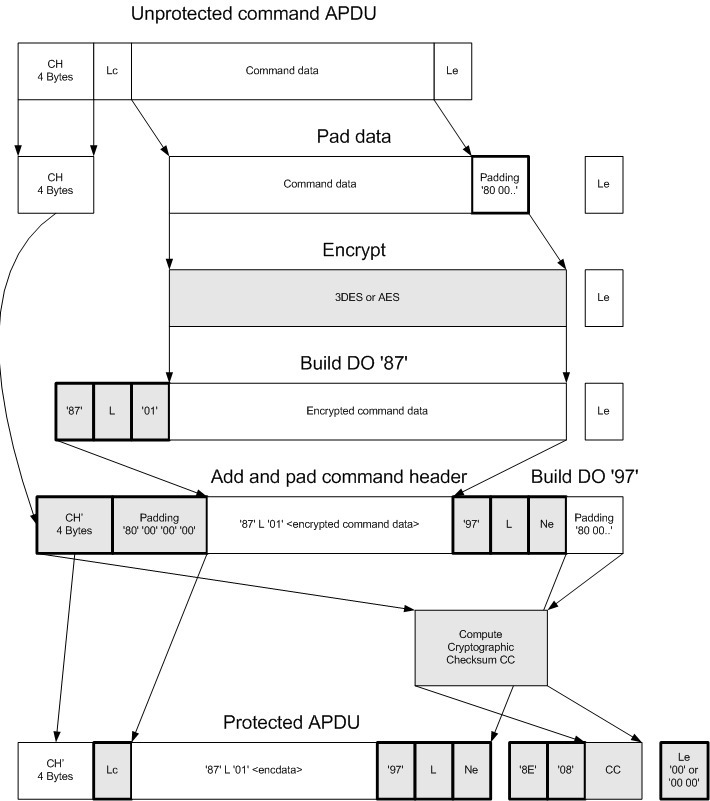
\includegraphics[width=1\linewidth]
  {images/section_7/7.3/sm_command.png}
\end{subfigure}
\caption{How to build APDU commands within secure messaging}
\end{figure}

% IMAGE: SM response
\begin{figure}[H]
\centering
\begin{subfigure}{1\textwidth}
  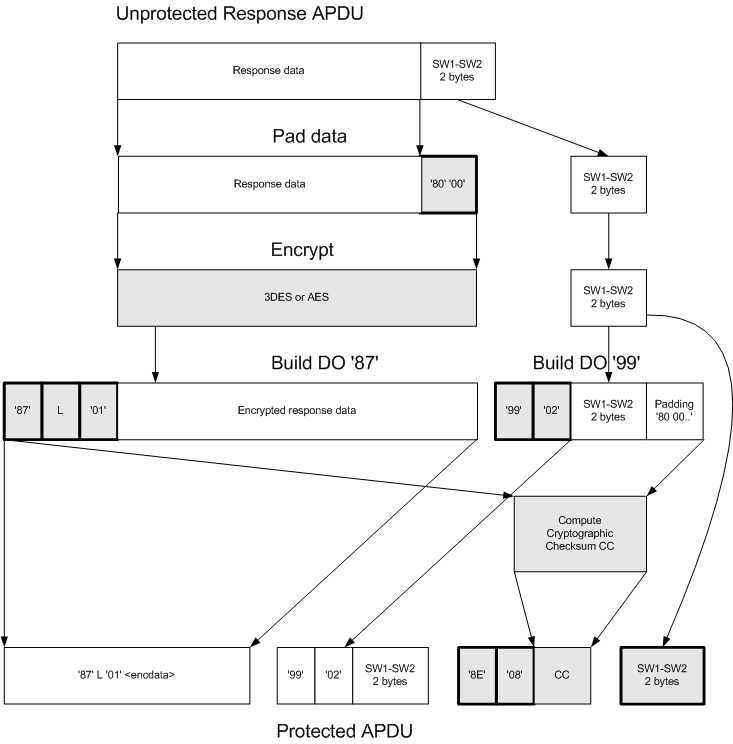
\includegraphics[width=1\linewidth]
  {images/section_7/7.3/sm_response.png}
\end{subfigure}
\caption{How to build APDU response's within secure messaging}
\end{figure}

The paper also suggests that only triple DES or AES block ciphers are used within secure messaging. Using the knowledge from the traces we have of the smartcard we analyse, we can now deduce with that the checksum (CMAC) is of length 8 bytes. This therefore rules out the possibility of the use of AES, and only leaves triple DES. Triple DES has 3 key options. We reported earlier that the first 16 bytes of the cards 32 byte challenge is used for deriving S$_{Enc}$, and the second 16 bytes for S$_{Mac}$. Considering it is 16 bytes, and not 8 nor 24, we make the assumption that key option 2 for triple DES is used for secure messaging.

\begin{table}[H]
\begin{tabular}{|l|l|l|c|}
\hline
Block Cipher & Key size & Block Size & Used in Secure Messaging\\
\hline
AES & 16 & 16 & $\chi$\\
\hline
DES \textit{(key option 1)} & 8 & 8 & $\chi$\\
\hline
\textbf{DES \textit{(key option 2)}} & \textbf{16} & \textbf{8} & \checked\\
\hline
DES \textit{(key option 3)} & 24 & 8 & $\chi$\\
\hline
\end{tabular}
\end{table}

Based on this knowledge we now can build the encrypted command for 'GET CHALLENGE' with different generated keys, using DES3 (key option 2) separately. The only part left to do is to generate session keys using different key derivation functions. Unfortunately due to time constraints we have not been able to complete this part of the experiment and therefore the reverse engineering of the secure messaging protocol. We will however explain the key derivation functions (KDF) we think should be tested, and how to conduct the tests.

The first step in the experiment is to generate session keys using the 32 byte challenge from the card and the shared secret from the diffie hellman protocol. We report these two values below in table 7.16. We also need to re-introduce the hash functions that the card supports as these will be utilised for the KDF's, for generating the session keys, these are reported in table 7.17.

\begin{table}[H]
\begin{tabular}{|p{4cm}|p{10cm}|}
\hline
\textbf{Variable} & \textbf{Value}\\
\hline
First 16 bytes of 32 byte card challenge (denoted \textbf{cc\_1}) & C8 04 C7 25 A9 14 2D 58 E8 01 64 6D 72 DA C4 9C\\
\hline
Second 16 bytes of 32 byte card challenge (denoted \textbf{cc\_2}) & A5 F0 D1 FA AF 53 93 A7 49 8D 69 8B 7A 1A D0 A4\\
\hline
Shared secret (denote \textbf{ss}) & 00\\
\hline
\end{tabular}
\caption{Key generation parameters}
\end{table}

% TABLE: Hash functions
\begin{table}[H]
\begin{center}
\begin{tabular}{|c|c|c|}
\hline
Hash Name & Output Length (bits) & Output Length (Bytes)\\
\hline

MD5 & 128 &16\\
SHA1 & 160 & 20\\
SHA256 & 256 & 32\\
SHA384 & 384 & 48\\
SHA512 & 512 & 64\\
\hline
\end{tabular}
\caption{Hash Functions \textit{(supported by the card)}}
\end{center}
\end{table}

Using the data above we can now generate session keys S$_{Enc}$ and S$_{Mac}$ using the following key derivation techniques:

\begin{table}[H]
\begin{tabular}{|c|l|l|}
\hline
KDF & S$_{Enc}$ & S$_{Mac}$\\
\hline
1 & Truncate(ss XOR cc\_1) & Truncate(ss XOR cc\_2)\\
\hline
2 & Truncate(Hash(ss $||$ cc\_1)) & Truncate(Hash(ss $||$ cc\_2)) \\
\hline
3 & Truncate(Hash(ss) XOR cc\_1) & Truncate(Hash(ss) XOR cc\_2)\\
\hline
4 & Truncate(Hash(ss$||$cc\_1$||$cc\_2))[0:16] & Truncate(Hash(ss$||$cc\_1$||$cc\_2))[16:32]\\
\hline
5 & Truncate(Hash(s))[0:16] XOR cc\_1 & Truncate(Hash(ss))[16:32] XOR cc\_2\\
\hline
\end{tabular}
\caption{Methods for generation session keys}
\end{table}

\textit{[Note that for KDF 4 and 5, the hash functions used must have an output size greater than or equal too 32 bytes. Thus MD5 and sha1 cannot be utilised.]}

With the generated session keys S$_{Enc}$ and S$_{Mac}$ we now build the encrypted command for 'GET CHALLENGE' for comparison against the command that is already been generated by the API. To build to command we follow the steps that are in figure 7.4. Since the data field of the 'GET CHALLENGE' command is empty we only need to compute the checksum (CMAC) of the entire message. We by following these steps:

\begin{enumerate}
\item Block cipher = Triple DES - key option 2
\item Mode = C-MAC
\item IV = 00 00 00 00 00 00 00 00 
\item Password = S$_{Mac}$
\item Message = 0C 84 00 00 80 00 00 00 97 01 08 80 00 00 00 00
\end{enumerate}

$$ Checksum \quad = \quad encrypt(Message) $$

Encrypted command = 0C 84 00 00 0D 97 01 18 8E 08 $Checksum$ 00\\

Once we find a match between the encrypted command we generate and the command the API encrypts we will know for sure that we have the correct session keys computed and thus will have successfully reversed engineered the secure messaging protocol. This concludes this section.

%---------------------------------------------------------------------------------------------------------------------------------------------------
\chapter{Conclusion / Results}

This shall summarise the whole report and my findings in regard to low-level vulnerabilities on the card. 

\chapter{Future work}

\begin{enumerate}
\item Complete the reverse engineering secure messaging
\item Decrypt and understand the unwrap command
\item Test and get the wrap command to work (hopefully)
\item Implement the wrap/decrypt attack at the APDU level.

\item Try using 'reallocate binary' and/or 'delete file' then 'create file' (must be done with caution! could brick card) to alter the retry counter for logging in. (Then a successful login trace is not required!)
\end{enumerate}

%---------------------------------------------------------------------------------------------------------------------------------------------------
%---------------------------------------------------------------------------------------------------------------------------------------------------
% use the following and \cite{} as above if you use BibTeX
% otherwise generate bibtem entries
\bibliographystyle{plain}
%\bibliography{mybib}
\begin{thebibliography}{}

%-------------------------------------------------------------------------------
% EXAMPLES!!
\bibitem{latexcompanion} 
Michel Goossens, Frank Mittelbach, and Alexander Samarin. 
\textit{The \LaTeX\ Companion}. 
Addison-Wesley, Reading, Massachusetts, 1993.
 
\bibitem{einstein} 
Albert Einstein. 
\textit{Zur Elektrodynamik bewegter K{\"o}rper}. (German) 
[\textit{On the electrodynamics of moving bodies}]. 
Annalen der Physik, 322(10):891–921, 1905.
 
\bibitem{knuthwebsite} 
Knuth: Computers and Typesetting,
\\\texttt{http://www-cs-faculty.stanford.edu/\~{}uno/abcde.html}
%------------------------------------------------------------------------------

\bibitem{virtual smartcard}
Frank Morgner : Creating a Virtual Smart Card\\
\texttt{https://frankmorgner.github.io/vsmartcard/virtualsmartcard/README.html}\\
%\href{https://frankmorgner.github.io/vsmartcard/virtualsmartcard/README.html}{link}

\bibitem{OCRA}
Internet Engineering Task Force (IETF).\\
\textit{OCRA: OATH Challenge-Response Algorithm}, June 2011\\
\texttt{https://tools.ietf.org/html/rfc6287}


\end{thebibliography}


\begin{appendices}
\chapter{Attack Traces}

\section{Multiple C\_login Traces}
\subsection{Different Second}
\begin{Verbatim}[commandchars=\\\{\}, fontsize=\small]
----- APDU command/response pair 0 -----
\textit{(Inter-Industry) Get Challenge}
00000000: 00 84 00 00 08                                    .....

00000000: \textbf{00 00 00 00 00 00 00 00}  90 00                    ..........

----- APDU command/response pair 1 -----
\textit{(Proprietary) Verify}
00000000: 80 20 00 00 10 \textbf{61 50 65  E1 AF 05 7B C3 35 98 0D}  . ...aPe...\{.5..
00000010: \textbf{DC 9D C5 42 96}                                    ...B.

00000000: 63 C9                                             c.

----- APDU command/response pair 1 -----
\textit{(Inter-Industry) Get Challenge}
00000000: 00 84 00 00 08                                    .....

00000000: \textbf{00 00 00 00 00 00 00 00}  90 00                    ..........

----- APDU command/response pair 1 -----
\textit{(Proprietary) Verify}
00000000: 80 20 00 00 10 \textbf{BF 73 83  F9 30 B1 74 D2 E4 98 83}  . ....s..0.t....
00000010: \textbf{3A 9F 1F 37 BA}                                    :..7.

00000000: 63 C8                                             c.
\end{Verbatim}
\subsection{Same Pin, Same Challenge}
\begin{Verbatim}[commandchars=\\\{\}, fontsize=\small]
----- APDU command/response pair 0 -----
\textit{(Inter-Industry) Get Challenge}
00000000: 00 84 00 00 08                                    .....

00000000: \textbf{00 00 00 00 00 00 00 00}  90 00                    ..........

----- APDU command/response pair 1 -----
\textit{(Proprietary) Verify}
00000000: 80 20 00 00 10 \textbf{EE D2 F1  54 07 18 8A 8F AB A3 F7}  . ......T.......
00000010: \textbf{3E 64 17 2D 6E}                                    >d.-n

00000000: 63 C9                                             c.

----- APDU command/response pair 1 -----
\textit{(Inter-Industry) Get Challenge}
00000000: 00 84 00 00 08                                    .....

00000000: \textbf{00 00 00 00 00 00 00 00}  90 00                    ..........

----- APDU command/response pair 1 -----
\textit{(Proprietary) Verify}
00000000: 80 20 00 00 10 \textbf{EE D2 F1  54 07 18 8A 8F AB A3 F7}  . ......T.......
00000010: \textbf{3E 64 17 2D 6E}                                    >d.-n

00000000: 63 C8                                             c.

\end{Verbatim}
\subsection{Same Pin, Different Challenge}
\begin{Verbatim}[commandchars=\\\{\}, fontsize=\small]
----- APDU command/response pair 0 -----
\textit{(Inter-Industry) Get Challenge}
00000000: 00 84 00 00 08                                    .....

00000000: \textbf{00 00 00 00 00 00 00 00}  90 00                    ..........

----- APDU command/response pair 1 -----
\textit{(Proprietary) Verify}
00000000: 80 20 00 00 10 \textbf{6E 78 D4  D5 61 AD 3C 26 D3 89 E8}  . ...nx..a.<&...
00000010: \textbf{96 B9 92 0D 40}                                    ....@

00000000: 63 C9                                             c.

----- APDU command/response pair 1 -----
\textit{(Inter-Industry) Get Challenge}
00000000: 00 84 00 00 08                                    .....

00000000: \textbf{00 00 00 00 00 00 00 01}  90 00                    ..........

----- APDU command/response pair 1 -----
\textit{(Proprietary) Verify}
00000000: 80 20 00 00 10 \textbf{6E 78 D4  D5 61 AD 3C 26 BC C6 AA}  . ...nx..a.<&...
00000010: \textbf{72 D3 95 2B 94}                                    r..+.

00000000: 63 C8                                             c.

\end{Verbatim}
\subsection{Different Pin, Same Challenge}
\begin{Verbatim}[commandchars=\\\{\}, fontsize=\small]
----- APDU command/response pair 0 -----
\textit{(Inter-Industry) Get Challenge}
00000000: 00 84 00 00 08                                    .....

00000000: \textbf{00 00 00 00 00 00 00 00}  90 00                    ..........

----- APDU command/response pair 1 -----
\textit{(Proprietary) Verify}
00000000: 80 20 00 00 10 \textbf{8F 58 1B  91 BC 78 D3 37 A9 D9 FB}  . ....X...x.7...
00000010: \textbf{9C 20 58 F6 0A}                                    . X..

00000000: 63 C9                                             c.

----- APDU command/response pair 1 -----
\textit{(Inter-Industry) Get Challenge}
00000000: 00 84 00 00 08                                    .....

00000000: \textbf{00 00 00 00 00 00 00 00}  90 00                    ..........

----- APDU command/response pair 1 -----
\textit{(Proprietary) Verify}
00000000: 80 20 00 00 10 \textbf{E0 30 33  BB 03 0F 6E 11 08 C0 8D}  . ....03...n....
00000010: \textbf{1D 9D 85 C4 A6}                                    .....

00000000: 63 C8                                             c.

\end{Verbatim}
\subsection{Different Pin, Different Challenge}
\begin{Verbatim}[commandchars=\\\{\}, fontsize=\small]
----- APDU command/response pair 0 -----
\textit{(Inter-Industry) Get Challenge}
00000000: 00 84 00 00 08                                    .....

00000000: \textbf{00 00 00 00 00 00 00 00}  90 00                    ..........

----- APDU command/response pair 1 -----
\textit{(Proprietary) Verify}
00000000: 80 20 00 00 \textbf{10 C2 29 5F  78 D1 68 29 13 78 BE 7B}  . ....)_x.h).x.\{
00000010: \textbf{8E 61 9B 32 2E}                                    .a.2.

00000000: 63 C9                                             c.

----- APDU command/response pair 1 -----
\textit{(Inter-Industry) Get Challenge}
00000000: 00 84 00 00 08                                    .....

00000000: \textbf{00 00 00 00 00 00 00 01}  90 00                    ..........

----- APDU command/response pair 1 -----
\textit{(Proprietary) Verify}
00000000: 80 20 00 00 10 \textbf{C4 6D 44  03 92 F3 6B EF 13 18 07}  . ....mD...k....
00000010: \textbf{CE 5A A4 B9 27}                                    .Z..'

00000000: 63 C8                                             c.
\end{Verbatim}
\section{Successful Login Injection}
\begin{Verbatim}[commandchars=\\\{\}, fontsize=\small]
----- APDU command/response pair 12 -----

\textit{(Inter-Industry) Get Challenge}
COMMAND from API
00000000: 00 84 00 00 08                                    .....

Do you want to automate the injection your own login response? (Y/n)

RESPONSE
00000000: E7 69 60 B5 C8 FC D2 02  90 00                    .i`.......

----- APDU command/response pair 13 -----

\textit{(Proprietary) Verify}
COMMAND from API
00000000: 80 20 00 00 10 \textbf{4A D1 3D  AB 98 7F C5 18 A9 B3 1F}  . ...J.=........
00000010: \textbf{2F 96 B4 3C AF}                                    /..<.

\textit{(Proprietary) Verify}
COMMAND injected
00000000: 80 20 00 00 10 \textbf{32 5A 9F  38 CA 4F BE 44 3A CD E1}  . ...2Z.8.O.D:..
00000010: \textbf{C5 03 84 35 DF}                                    ...5.

RESPONSE
00000000: 90 00                                             ..
\end{Verbatim}

\section{Open Secure Messaging Traces}
\subsection{Generator = 5, [Not modified]}
\begin{Verbatim}[commandchars=\\\{\}, fontsize=\small]
----- APDU command/response pair 24 -----

\textit{(Proprietary) Get Card Public Key}
COMMAND from API
00000000: 80 48 00 80 00                                    .H...

Do you want to to alter command? (y/N)

RESPONSE
00000000: \textbf{80 01 05 81 81 80} F7 B5  15 72 07 22 94 6F C4 08  .........r.".o..
00000010: 64 CB BD AF EA 55 7D BD  8F 55 36 B0 01 C2 8B 2E  d....U\}..U6.....
00000020: 32 B6 5D 45 F1 74 5D 38  12 0B AD 9D 2C 03 9C 22  2.]E.t]8....,.."
00000030: 46 68 EB 2E A2 8C 20 95  A8 2E 6C A8 E0 6D 47 F2  Fh.... ...l..mG.
00000040: D3 1E D7 01 F8 15 5C AD  DC 05 70 C0 93 B2 6D 74  ......\...p...mt
00000050: B0 9B 95 E6 4D 8C D2 FC  73 3E CD 0F 30 68 79 A5  ....M...s>..0hy.
00000060: B9 35 F2 41 3F 52 AD AD  32 A0 99 1A 18 3D CC 57  .5.A?R..2....=.W
00000070: 7E 39 DA 47 53 1E 67 15  AB 01 70 7F F2 47 96 71  ~9.GS.g...p..G.q
00000080: 44 23 CE 7B 60 67 \textbf{82 81  80} 3C 52 D2 06 89 28 92  D#.\{`g...<R...(.
00000090: 2C AB E6 3C 4E E6 DF 0E  D2 29 F1 01 BE 36 C4 F8  ,..<N....)...6..
000000A0: 54 40 56 F3 4A FA 8D 2E  9B 60 F5 07 BC ED B4 44  T@V.J....`.....D
000000B0: 56 68 5D 82 4C C4 EA D7  96 20 F8 C5 46 A6 E0 16  Vh].L.... ..F...
000000C0: B8 AB A5 D8 43 29 58 53  77 17 09 97 AA 70 68 33  ....C)XSw....ph3
000000D0: 9E F1 41 0A 5F 39 D9 75  24 7F 3A 53 63 61 47 87  ..A.\_9.u\$.:ScaG.
000000E0: 87 7F 88 96 BC BB 83 A1  CB D1 42 E0 EB 99 CF 34  ..........B....4
000000F0: 0E CA 56 4F 2C 57 50 6E  7B 1A FC 1F 90 7A E0 C2  ..VO,WPn\{....z..
00000100: 61 09                                             a.

Do you want to alter the response? (y/N)

----- APDU command/response pair 25 -----

\textit{(Inter-Industry) Get Remaining Bytes}
COMMAND from API
00000000: 00 C0 00 00 09                                    .....

Do you want to to alter command? (y/N)

RESPONSE
00000000: A8 5D D3 30 E3 5C A9 00  39 90 00                 .].0....9..

Do you want to alter the response? (y/N)

----- APDU command/response pair 26 -----

\textit{(Proprietary) Open Secure Messaging}
COMMAND from API
\textbf{00000000: 80 86 00 00 80 08 9F EA  A1 DC 8F C3 43 FD FD 4A  ............C..J}
\textbf{00000010: E6 95 7E C0 D3 C6 FE 81  61 59 4B CE 45 21 96 63  ..~.....aYK.E!.c}
\textbf{00000020: 0F AB 19 D8 61 1A B2 6B  00 E2 44 0F 06 A3 5B 60  ....a..k..D...[`}
\textbf{00000030: 87 76 C0 B7 E9 15 D5 50  DB 17 D6 C1 3C 26 54 47  .v.....P....<&TG}
\textbf{00000040: AA A3 4B DC 2C 14 81 08  84 0D F0 CA FB 49 8B C1  ..K.,........I..}
\textbf{00000050: B1 0B A1 2B 86 20 02 F2  0F 69 F0 56 2C 83 0C 6E  ...+. ...i.V,..n}
\textbf{00000060: A6 6A E9 86 56 47 71 24  0C B7 91 7F 37 85 0A D4  .j..VGq\$....7...}
\textbf{00000070: 12 35 1F CE 17 6C D2 52  FB 04 24 CF DD E9 53 BE  .5...l.R..\$...S.}
\textbf{00000080: DA 26 EA 54 FB 00                                 .&.T..}
Do you want to to alter command? (y/N)

RESPONSE
00000000: 66 56 36 31 16 42 8D 8A  BC 06 BA AC 5D 35 26 F5  fV61.B......]5&.
00000010: BF 58 15 7F 00 4F EF 2F  54 FB C4 F2 10 8F CB D6  .X...O./T.......
00000020: 90 00                                             ..

Do you want to alter the response? (y/N)

----- APDU command/response pair 27 -----

\textit{(Proprietary) Get Challenge [SM]}
COMMAND from API
00000000: 0C 84 00 00 0D 97 01 20  8E 08 05 E4 4A 19 32 DE  ....... ....J.2.
00000010: 51 CB 00                                          Q..

Do you want to to alter command? (y/N)

RESPONSE
00000000: 87 29 01 BD 69 F3 85 A7  98 2E 08 07 21 88 30 2F  .)..i.......!.0/
00000010: 06 FF 93 E4 2F 31 C5 4A  40 FB 45 3A 45 C1 4A 84  ..../1.J@.E:E.J.
00000020: 7F BA 59 BC 44 8A 70 A0  BC DA FB 99 02 90 00 8E  ..Y.D.p.........
00000030: 08 44 26 95 74 6A 51 A3  72 90 00                 .D&.tjQ.r..

Do you want to alter the response? (y/N)

----- APDU command/response pair 28 -----

\textit{(Proprietary) Close Secure Messaging}
COMMAND from API
00000000: 80 86 FF FF                                       ....
\end{Verbatim}
\subsection{Generator = 1}
\begin{Verbatim}[commandchars=\\\{\}, fontsize=\small]
----- APDU command/response pair 24 -----

\textit{(Proprietary) Get Card Public Key}
COMMAND from API
00000000: 80 48 00 80 00                                    .H...

Do you want to to alter command? (y/N)

RESPONSE
00000000: \textbf{80 01 05 81 81 80} F7 B5  15 72 07 22 94 6F C4 08  .........r.".o..
00000010: 64 CB BD AF EA 55 7D BD  8F 55 36 B0 01 C2 8B 2E  d....U\}..U6.....
00000020: 32 B6 5D 45 F1 74 5D 38  12 0B AD 9D 2C 03 9C 22  2.]E.t]8....,.."
00000030: 46 68 EB 2E A2 8C 20 95  A8 2E 6C A8 E0 6D 47 F2  Fh.... ...l..mG.
00000040: D3 1E D7 01 F8 15 5C AD  DC 05 70 C0 93 B2 6D 74  ......\...p...mt
00000050: B0 9B 95 E6 4D 8C D2 FC  73 3E CD 0F 30 68 79 A5  ....M...s>..0hy.
00000060: B9 35 F2 41 3F 52 AD AD  32 A0 99 1A 18 3D CC 57  .5.A?R..2....=.W
00000070: 7E 39 DA 47 53 1E 67 15  AB 01 70 7F F2 47 96 71  ~9.GS.g...p..G.q
00000080: 44 23 CE 7B 60 67 \textbf{82 81  80} 3C 52 D2 06 89 28 92  D#.\{`g...<R...(.
00000090: 2C AB E6 3C 4E E6 DF 0E  D2 29 F1 01 BE 36 C4 F8  ,..<N....)...6..
000000A0: 54 40 56 F3 4A FA 8D 2E  9B 60 F5 07 BC ED B4 44  T@V.J....`.....D
000000B0: 56 68 5D 82 4C C4 EA D7  96 20 F8 C5 46 A6 E0 16  Vh].L.... ..F...
000000C0: B8 AB A5 D8 43 29 58 53  77 17 09 97 AA 70 68 33  ....C)XSw....ph3
000000D0: 9E F1 41 0A 5F 39 D9 75  24 7F 3A 53 63 61 47 87  ..A.\_9.u\$.:ScaG.
000000E0: 87 7F 88 96 BC BB 83 A1  CB D1 42 E0 EB 99 CF 34  ..........B....4
000000F0: 0E CA 56 4F 2C 57 50 6E  7B 1A FC 1F 90 7A E0 C2  ..VO,WPn\{....z..
00000100: 61 09                                             a.

Do you want to alter the response? (y/N)
y

00000000: 80 01 \textbf{01} 81 81 80 F7 B5  15 72 07 22 94 6F C4 08  .........r.".o..
00000010: 64 CB BD AF EA 55 7D BD  8F 55 36 B0 01 C2 8B 2E  d....U\}..U6.....
00000020: 32 B6 5D 45 F1 74 5D 38  12 0B AD 9D 2C 03 9C 22  2.]E.t]8....,.."
00000030: 46 68 EB 2E A2 8C 20 95  A8 2E 6C A8 E0 6D 47 F2  Fh.... ...l..mG.
00000040: D3 1E D7 01 F8 15 5C AD  DC 05 70 C0 93 B2 6D 74  ......\...p...mt
00000050: B0 9B 95 E6 4D 8C D2 FC  73 3E CD 0F 30 68 79 A5  ....M...s>..0hy.
00000060: B9 35 F2 41 3F 52 AD AD  32 A0 99 1A 18 3D CC 57  .5.A?R..2....=.W
00000070: 7E 39 DA 47 53 1E 67 15  AB 01 70 7F F2 47 96 71  ~9.GS.g...p..G.q
00000080: 44 23 CE 7B 60 67 82 81  80 3C 52 D2 06 89 28 92  D#.\{`g...<R...(.
00000090: 2C AB E6 3C 4E E6 DF 0E  D2 29 F1 01 BE 36 C4 F8  ,..<N....)...6..
000000A0: 54 40 56 F3 4A FA 8D 2E  9B 60 F5 07 BC ED B4 44  T@V.J....`.....D
000000B0: 56 68 5D 82 4C C4 EA D7  96 20 F8 C5 46 A6 E0 16  Vh].L.... ..F...
000000C0: B8 AB A5 D8 43 29 58 53  77 17 09 97 AA 70 68 33  ....C)XSw....ph3
000000D0: 9E F1 41 0A 5F 39 D9 75  24 7F 3A 53 63 61 47 87  ..A.\_9.u\$.:ScaG.
000000E0: 87 7F 88 96 BC BB 83 A1  CB D1 42 E0 EB 99 CF 34  ..........B....4
000000F0: 0E CA 56 4F 2C 57 50 6E  7B 1A FC 1F 90 7A E0 C2  ..VO,WPn\{....z..
00000100: 61 09                                             a.
response changed!

----- APDU command/response pair 25 -----

\textit{(Inter-Industry) Get Remaining Bytes}
COMMAND from API
00000000: 00 C0 00 00 09                                    .....

Do you want to to alter command? (y/N)

RESPONSE
00000000: A8 5D D3 30 E3 5C A9 00  39 90 00                 .].0....9..

Do you want to alter the response? (y/N)

----- APDU command/response pair 26 -----

\textit{(Proprietary) Open Secure Messaging}
COMMAND from API
\textbf{00000000: 80 86 00 00 80 00 00 00  00 00 00 00 00 00 00 00  ................}
\textbf{00000010: 00 00 00 00 00 00 00 00  00 00 00 00 00 00 00 00  ................}
\textbf{00000020: 00 00 00 00 00 00 00 00  00 00 00 00 00 00 00 00  ................}
\textbf{00000030: 00 00 00 00 00 00 00 00  00 00 00 00 00 00 00 00  ................}
\textbf{00000040: 00 00 00 00 00 00 00 00  00 00 00 00 00 00 00 00  ................}
\textbf{00000050: 00 00 00 00 00 00 00 00  00 00 00 00 00 00 00 00  ................}
\textbf{00000060: 00 00 00 00 00 00 00 00  00 00 00 00 00 00 00 00  ................}
\textbf{00000070: 00 00 00 00 00 00 00 00  00 00 00 00 00 00 00 00  ................}
\textbf{00000080: 00 00 00 00 01 00                                 ......}

Do you want to to alter command? (y/N)

RESPONSE
00000000: 7D 2C 25 47 1C 16 34 51  E9 C3 49 38 C8 79 1E ED  \},\%G..4Q..I8.y..
00000010: A2 6B 20 D4 54 BD 67 0A  D3 85 3E B9 E0 6E D5 5E  .k .T.g...>..n.^
00000020: 90 00                                             ..

Do you want to alter the response? (y/N)

----- APDU command/response pair 27 -----

\textit{(Proprietary) Get Challenge [SM]}
COMMAND from API
00000000: 0C 84 00 00 0D 97 01 20  8E 08 08 C6 59 9B 57 E6  ....... ....Y.W.
00000010: B4 4E 00                                          .N.

Do you want to to alter command? (y/N)

RESPONSE
00000000: 69 88                                             i.

Do you want to alter the response? (y/N)

----- APDU command/response pair 28 -----

\textit{(Proprietary) Close Secure Messaging}
COMMAND from API
00000000: 80 86 FF FF                                       ....
\end{Verbatim}
\subsection{Generator = 0}
\begin{Verbatim}[commandchars=\\\{\}, fontsize=\small]
----- APDU command/response pair 24 -----

\textit{(Proprietary) Get Card Public Key}
COMMAND from API
00000000: 80 48 00 80 00                                    .H...

Do you want to to alter command? (y/N)

RESPONSE
00000000: \textbf{80 01 05 81 81 80} F7 B5  15 72 07 22 94 6F C4 08  .........r.".o..
00000010: 64 CB BD AF EA 55 7D BD  8F 55 36 B0 01 C2 8B 2E  d....U\}..U6.....
00000020: 32 B6 5D 45 F1 74 5D 38  12 0B AD 9D 2C 03 9C 22  2.]E.t]8....,.."
00000030: 46 68 EB 2E A2 8C 20 95  A8 2E 6C A8 E0 6D 47 F2  Fh.... ...l..mG.
00000040: D3 1E D7 01 F8 15 5C AD  DC 05 70 C0 93 B2 6D 74  ......\...p...mt
00000050: B0 9B 95 E6 4D 8C D2 FC  73 3E CD 0F 30 68 79 A5  ....M...s>..0hy.
00000060: B9 35 F2 41 3F 52 AD AD  32 A0 99 1A 18 3D CC 57  .5.A?R..2....=.W
00000070: 7E 39 DA 47 53 1E 67 15  AB 01 70 7F F2 47 96 71  ~9.GS.g...p..G.q
00000080: 44 23 CE 7B 60 67 \textbf{82 81  80} 3C 52 D2 06 89 28 92  D#.\{`g...<R...(.
00000090: 2C AB E6 3C 4E E6 DF 0E  D2 29 F1 01 BE 36 C4 F8  ,..<N....)...6..
000000A0: 54 40 56 F3 4A FA 8D 2E  9B 60 F5 07 BC ED B4 44  T@V.J....`.....D
000000B0: 56 68 5D 82 4C C4 EA D7  96 20 F8 C5 46 A6 E0 16  Vh].L.... ..F...
000000C0: B8 AB A5 D8 43 29 58 53  77 17 09 97 AA 70 68 33  ....C)XSw....ph3
000000D0: 9E F1 41 0A 5F 39 D9 75  24 7F 3A 53 63 61 47 87  ..A.\_9.u\$.:ScaG.
000000E0: 87 7F 88 96 BC BB 83 A1  CB D1 42 E0 EB 99 CF 34  ..........B....4
000000F0: 0E CA 56 4F 2C 57 50 6E  7B 1A FC 1F 90 7A E0 C2  ..VO,WPn\{....z..
00000100: 61 09                                             a.

Do you want to alter the response? (y/N)
y

00000000: 80 01 \textbf{00} 81 81 80 F7 B5  15 72 07 22 94 6F C4 08  .........r.".o..
00000010: 64 CB BD AF EA 55 7D BD  8F 55 36 B0 01 C2 8B 2E  d....U\}..U6.....
00000020: 32 B6 5D 45 F1 74 5D 38  12 0B AD 9D 2C 03 9C 22  2.]E.t]8....,.."
00000030: 46 68 EB 2E A2 8C 20 95  A8 2E 6C A8 E0 6D 47 F2  Fh.... ...l..mG.
00000040: D3 1E D7 01 F8 15 5C AD  DC 05 70 C0 93 B2 6D 74  ......\...p...mt
00000050: B0 9B 95 E6 4D 8C D2 FC  73 3E CD 0F 30 68 79 A5  ....M...s>..0hy.
00000060: B9 35 F2 41 3F 52 AD AD  32 A0 99 1A 18 3D CC 57  .5.A?R..2....=.W
00000070: 7E 39 DA 47 53 1E 67 15  AB 01 70 7F F2 47 96 71  ~9.GS.g...p..G.q
00000080: 44 23 CE 7B 60 67 82 81  80 3C 52 D2 06 89 28 92  D#.\{`g...<R...(.
00000090: 2C AB E6 3C 4E E6 DF 0E  D2 29 F1 01 BE 36 C4 F8  ,..<N....)...6..
000000A0: 54 40 56 F3 4A FA 8D 2E  9B 60 F5 07 BC ED B4 44  T@V.J....`.....D
000000B0: 56 68 5D 82 4C C4 EA D7  96 20 F8 C5 46 A6 E0 16  Vh].L.... ..F...
000000C0: B8 AB A5 D8 43 29 58 53  77 17 09 97 AA 70 68 33  ....C)XSw....ph3
000000D0: 9E F1 41 0A 5F 39 D9 75  24 7F 3A 53 63 61 47 87  ..A.\_9.u\$.:ScaG.
000000E0: 87 7F 88 96 BC BB 83 A1  CB D1 42 E0 EB 99 CF 34  ..........B....4
000000F0: 0E CA 56 4F 2C 57 50 6E  7B 1A FC 1F 90 7A E0 C2  ..VO,WPn\{....z..
00000100: 61 09                                             a.
response changed!

----- APDU command/response pair 25 -----

\textit{(Inter-Industry) Get Remaining Bytes}
COMMAND from API
00000000: 00 C0 00 00 09                                    .....

Do you want to to alter command? (y/N)

RESPONSE
00000000: A8 5D D3 30 E3 5C A9 00  39 90 00                 .].0....9..

Do you want to alter the response? (y/N)

----- APDU command/response pair 26 -----

\textit{(Proprietary) Open Secure Messaging}
COMMAND from API
\textbf{00000000: 80 86 00 00 80 00 00 00  00 00 00 00 00 00 00 00  ................}
\textbf{00000010: 00 00 00 00 00 00 00 00  00 00 00 00 00 00 00 00  ................}
\textbf{00000020: 00 00 00 00 00 00 00 00  00 00 00 00 00 00 00 00  ................}
\textbf{00000030: 00 00 00 00 00 00 00 00  00 00 00 00 00 00 00 00  ................}
\textbf{00000040: 00 00 00 00 00 00 00 00  00 00 00 00 00 00 00 00  ................}
\textbf{00000050: 00 00 00 00 00 00 00 00  00 00 00 00 00 00 00 00  ................}
\textbf{00000060: 00 00 00 00 00 00 00 00  00 00 00 00 00 00 00 00  ................}
\textbf{00000070: 00 00 00 00 00 00 00 00  00 00 00 00 00 00 00 00  ................}
\textbf{00000080: 00 00 00 00 00 00                                 ......}

Do you want to to alter command? (y/N)

RESPONSE
00000000: 7E 4B 40 E6 E3 B1 5D 25  2B 02 48 50 B3 63 CC 9E  ~K@...]\%+.HP.c..
00000010: 79 41 34 FC 04 B3 57 1C  06 E3 D1 36 3C 24 45 8D  yA4...W....6<\$E.
00000020: 90 00                                             ..

Do you want to alter the response? (y/N)

----- APDU command/response pair 27 -----

\textit{(Proprietary) Get Challenge [SM]}
COMMAND from API
00000000: 0C 84 00 00 0D 97 01 20  8E 08 99 BD 52 69 31 DD  ....... ....Ri1.
00000010: DB FD 00                                          ...

Do you want to to alter command? (y/N)

RESPONSE
00000000: 69 88                                             i.

Do you want to alter the response? (y/N)

----- APDU command/response pair 28 -----

\textit{(Proprietary) Close Secure Messaging}
COMMAND from API
00000000: 80 86 FF FF                                       ....
\end{Verbatim}



\subsection{First 128 bytes set to zero and generator 0}
\begin{Verbatim}[commandchars=\\\{\}, fontsize=\small]
----- APDU command/response pair 26 -----

\textit{(Proprietary) Get Card Public Key}
COMMAND from API
00000000: 80 48 00 80 00                                    .H...

Do you want to to alter command? (y/N)

RESPONSE
00000000: \textbf{80 01 05 81 81 80} F7 B5  15 72 07 22 94 6F C4 08  .........r.".o..
00000010: 64 CB BD AF EA 55 7D BD  8F 55 36 B0 01 C2 8B 2E  d....U\}..U6.....
00000020: 32 B6 5D 45 F1 74 5D 38  12 0B AD 9D 2C 03 9C 22  2.]E.t]8....,.."
00000030: 46 68 EB 2E A2 8C 20 95  A8 2E 6C A8 E0 6D 47 F2  Fh.... ...l..mG.
00000040: D3 1E D7 01 F8 15 5C AD  DC 05 70 C0 93 B2 6D 74  ......\...p...mt
00000050: B0 9B 95 E6 4D 8C D2 FC  73 3E CD 0F 30 68 79 A5  ....M...s>..0hy.
00000060: B9 35 F2 41 3F 52 AD AD  32 A0 99 1A 18 3D CC 57  .5.A?R..2....=.W
00000070: 7E 39 DA 47 53 1E 67 15  AB 01 70 7F F2 47 96 71  ~9.GS.g...p..G.q
00000080: 44 23 CE 7B 60 67 \textbf{82 81  80} 3C 52 D2 06 89 28 92  D#.\{`g...<R...(.
00000090: 2C AB E6 3C 4E E6 DF 0E  D2 29 F1 01 BE 36 C4 F8  ,..<N....)...6..
000000A0: 54 40 56 F3 4A FA 8D 2E  9B 60 F5 07 BC ED B4 44  T@V.J....`.....D
000000B0: 56 68 5D 82 4C C4 EA D7  96 20 F8 C5 46 A6 E0 16  Vh].L.... ..F...
000000C0: B8 AB A5 D8 43 29 58 53  77 17 09 97 AA 70 68 33  ....C)XSw....ph3
000000D0: 9E F1 41 0A 5F 39 D9 75  24 7F 3A 53 63 61 47 87  ..A.\_9.u\$.:ScaG.
000000E0: 87 7F 88 96 BC BB 83 A1  CB D1 42 E0 EB 99 CF 34  ..........B....4
000000F0: 0E CA 56 4F 2C 57 50 6E  7B 1A FC 1F 90 7A E0 C2  ..VO,WPn\{....z..
00000100: 61 09                                             a.

Do you want to alter the response? (y/N)
y

\textbf{00000000: 80 01 00 81 81 80 00 00  00 00 00 00 00 00 00 00  ................}
\textbf{00000010: 00 00 00 00 00 00 00 00  00 00 00 00 00 00 00 00  ................}
\textbf{00000020: 00 00 00 00 00 00 00 00  00 00 00 00 00 00 00 00  ................}
\textbf{00000030: 00 00 00 00 00 00 00 00  00 00 00 00 00 00 00 00  ................}
\textbf{00000040: 00 00 00 00 00 00 00 00  00 00 00 00 00 00 00 00  ................}
\textbf{00000050: 00 00 00 00 00 00 00 00  00 00 00 00 00 00 00 00  ................}
\textbf{00000060: 00 00 00 00 00 00 00 00  00 00 00 00 00 00 00 00  ................}
\textbf{00000070: 00 00 00 00 00 00 00 00  00 00 00 00 00 00 00 00  ................}
\textbf{00000080: 00 00 00 00 00 00} 82 81  80 3C 52 D2 06 89 28 92  .........<R...(.
00000090: 2C AB E6 3C 4E E6 DF 0E  D2 29 F1 01 BE 36 C4 F8  ,..<N....)...6..
000000A0: 54 40 56 F3 4A FA 8D 2E  9B 60 F5 07 BC ED B4 44  T@V.J....`.....D
000000B0: 56 68 5D 82 4C C4 EA D7  96 20 F8 C5 46 A6 E0 16  Vh].L.... ..F...
000000C0: B8 AB A5 D8 43 29 58 53  77 17 09 97 AA 70 68 33  ....C)XSw....ph3
000000D0: 9E F1 41 0A 5F 39 D9 75  24 7F 3A 53 63 61 47 87  ..A.\_9.u\$.:ScaG.
000000E0: 87 7F 88 96 BC BB 83 A1  CB D1 42 E0 EB 99 CF 34  ..........B....4
000000F0: 0E CA 56 4F 2C 57 50 6E  7B 1A FC 1F 90 7A E0 C2  ..VO,WPn\{....z..
00000100: 61 09                                             a.
response changed!

----- APDU command/response pair 27 -----

\textit{(Inter-Industry) Get Remaining Bytes}
COMMAND from API
00000000: 00 C0 00 00 09                                    .....

Do you want to to alter command? (y/N)

RESPONSE
00000000: A8 5D D3 30 E3 5C A9 00  39 90 00                 .].0....9..

Do you want to alter the response? (y/N)

(Halts here)
\end{Verbatim}
\subsection{Second 128 bytes set to zero and generator 0}
\begin{Verbatim}[commandchars=\\\{\}, fontsize=\small]
----- APDU command/response pair 35 -----

\textit{(Proprietary) Get Card Public Key}
COMMAND from API
00000000: 80 48 00 80 00                                    .H...

Do you want to to alter command? (y/N)

RESPONSE
00000000: \textbf{80 01 05 81 81 80} F7 B5  15 72 07 22 94 6F C4 08  .........r.".o..
00000010: 64 CB BD AF EA 55 7D BD  8F 55 36 B0 01 C2 8B 2E  d....U\}..U6.....
00000020: 32 B6 5D 45 F1 74 5D 38  12 0B AD 9D 2C 03 9C 22  2.]E.t]8....,.."
00000030: 46 68 EB 2E A2 8C 20 95  A8 2E 6C A8 E0 6D 47 F2  Fh.... ...l..mG.
00000040: D3 1E D7 01 F8 15 5C AD  DC 05 70 C0 93 B2 6D 74  ......\...p...mt
00000050: B0 9B 95 E6 4D 8C D2 FC  73 3E CD 0F 30 68 79 A5  ....M...s>..0hy.
00000060: B9 35 F2 41 3F 52 AD AD  32 A0 99 1A 18 3D CC 57  .5.A?R..2....=.W
00000070: 7E 39 DA 47 53 1E 67 15  AB 01 70 7F F2 47 96 71  ~9.GS.g...p..G.q
00000080: 44 23 CE 7B 60 67 \textbf{82 81  80} 3C 52 D2 06 89 28 92  D#.\{`g...<R...(.
00000090: 2C AB E6 3C 4E E6 DF 0E  D2 29 F1 01 BE 36 C4 F8  ,..<N....)...6..
000000A0: 54 40 56 F3 4A FA 8D 2E  9B 60 F5 07 BC ED B4 44  T@V.J....`.....D
000000B0: 56 68 5D 82 4C C4 EA D7  96 20 F8 C5 46 A6 E0 16  Vh].L.... ..F...
000000C0: B8 AB A5 D8 43 29 58 53  77 17 09 97 AA 70 68 33  ....C)XSw....ph3
000000D0: 9E F1 41 0A 5F 39 D9 75  24 7F 3A 53 63 61 47 87  ..A.\_9.u\$.:ScaG.
000000E0: 87 7F 88 96 BC BB 83 A1  CB D1 42 E0 EB 99 CF 34  ..........B....4
000000F0: 0E CA 56 4F 2C 57 50 6E  7B 1A FC 1F 90 7A E0 C2  ..VO,WPn\{....z..
00000100: 61 09                                             a.

Do you want to alter the response? (y/N)
y

00000000: 80 01 \textbf{00} 81 81 80 F7 B5  15 72 07 22 94 6F C4 08  .........r.".o..
00000010: 64 CB BD AF EA 55 7D BD  8F 55 36 B0 01 C2 8B 2E  d....U\}..U6.....
00000020: 32 B6 5D 45 F1 74 5D 38  12 0B AD 9D 2C 03 9C 22  2.]E.t]8....,.."
00000030: 46 68 EB 2E A2 8C 20 95  A8 2E 6C A8 E0 6D 47 F2  Fh.... ...l..mG.
00000040: D3 1E D7 01 F8 15 5C AD  DC 05 70 C0 93 B2 6D 74  ......\...p...mt
00000050: B0 9B 95 E6 4D 8C D2 FC  73 3E CD 0F 30 68 79 A5  ....M...s>..0hy.
00000060: B9 35 F2 41 3F 52 AD AD  32 A0 99 1A 18 3D CC 57  .5.A?R..2....=.W
00000070: 7E 39 DA 47 53 1E 67 15  AB 01 70 7F F2 47 96 71  ~9.GS.g...p..G.q
00000080: 44 23 CE 7B 60 67 \textbf{82 81  80 00 00 00 00 00 00 00  D\#.\{`g..........}
\textbf{00000090: 00 00 00 00 00 00 00 00  00 00 00 00 00 00 00 00  ................}
\textbf{000000A0: 00 00 00 00 00 00 00 00  00 00 00 00 00 00 00 00  ................}
\textbf{000000B0: 00 00 00 00 00 00 00 00  00 00 00 00 00 00 00 00  ................}
\textbf{000000C0: 00 00 00 00 00 00 00 00  00 00 00 00 00 00 00 00  ................}
\textbf{000000D0: 00 00 00 00 00 00 00 00  00 00 00 00 00 00 00 00  ................}
\textbf{000000E0: 00 00 00 00 00 00 00 00  00 00 00 00 00 00 00 00  ................}
\textbf{000000F0: 00 00 00 00 00 00 00 00  00 00 00 00 00 00 00 00  ................}
\textbf{00000100: 61 09                                             a.}
response changed!

----- APDU command/response pair 36 -----

\textit{(Inter-Industry) Get Remaining Bytes}
COMMAND from API
00000000: 00 C0 00 00 09                                    .....

Do you want to to alter command? (y/N)

RESPONSE
00000000: A8 5D D3 30 E3 5C A9 00  39 90 00                 .].0....9..

Do you want to alter the response? (y/N)
y

\textbf{00000000: 00 00 00 00 00 00 00 00  00 90 00                 ...........}
response changed!

----- APDU command/response pair 37 -----

\textit{(Proprietary) Open Secure Messaging}
COMMAND from API
\textbf{00000000: 80 86 00 00 80 00 00 00  00 00 00 00 00 00 00 00  ................}
\textbf{00000010: 00 00 00 00 00 00 00 00  00 00 00 00 00 00 00 00  ................}
\textbf{00000020: 00 00 00 00 00 00 00 00  00 00 00 00 00 00 00 00  ................}
\textbf{00000030: 00 00 00 00 00 00 00 00  00 00 00 00 00 00 00 00  ................}
\textbf{00000040: 00 00 00 00 00 00 00 00  00 00 00 00 00 00 00 00  ................}
\textbf{00000050: 00 00 00 00 00 00 00 00  00 00 00 00 00 00 00 00  ................}
\textbf{00000060: 00 00 00 00 00 00 00 00  00 00 00 00 00 00 00 00  ................}
\textbf{00000070: 00 00 00 00 00 00 00 00  00 00 00 00 00 00 00 00  ................}
\textbf{00000080: 00 00 00 00 00 00                                 ......}

Do you want to to alter command? (y/N)

RESPONSE
00000000: 22 2C 15 03 96 1F CA 12  4B CE CA 67 FE 92 5D A1  ",......K..g..].
00000010: 71 53 96 34 CD F3 10 8E  F9 2F 6F 28 CB E0 CE 78  qS.4...../o(...x
00000020: 90 00                                             ..

Do you want to alter the response? (y/N)

----- APDU command/response pair 38 -----

COMMAND from API
00000000: 0C 84 00 00 0D 97 01 20  8E 08 DF C1 4D 9E 7B 0A  ....... ....M.\{.
00000010: 24 E7 00                                          \$..

Do you want to to alter command? (y/N)

RESPONSE
00000000: 87 29 01 C7 40 87 51 07  6E 7A 62 89 6C 53 46 BC  .)..@.Q.nzb.lSF.
00000010: 4E 7A 2C E0 3B A7 A8 5B  44 90 4D 62 2C FB 1C 33  Nz,.;..[D.Mb,..3
00000020: 7D 18 CF 56 F8 76 8F 4C  E9 A2 F3 99 02 90 00 8E  \}..V.v.L........
00000030: 08 D1 DC BB 76 9A A7 6F  25 90 00                 ....v..o\%..

Do you want to alter the response? (y/N)

----- APDU command/response pair 39 -----

COMMAND from API
00000000: 80 86 FF FF                                       ....

Do you want to to alter command? (y/N)

RESPONSE
00000000: 90 00                                             ..
\end{Verbatim}

\subsection{Set 1st 16 bytes of card challenge to zero}
\begin{Verbatim}[commandchars=\\\{\}, fontsize=\small]
----- APDU command/response pair 24 -----

COMMAND from API
00000000: 80 48 00 80 00                                    .H...

Do you want to to alter command? (y/N)

RESPONSE
00000000: 80 01 05 81 81 80 F7 B5  15 72 07 22 94 6F C4 08  .........r.".o..
00000010: 64 CB BD AF EA 55 7D BD  8F 55 36 B0 01 C2 8B 2E  d....U\}..U6.....
00000020: 32 B6 5D 45 F1 74 5D 38  12 0B AD 9D 2C 03 9C 22  2.]E.t]8....,.."
00000030: 46 68 EB 2E A2 8C 20 95  A8 2E 6C A8 E0 6D 47 F2  Fh.... ...l..mG.
00000040: D3 1E D7 01 F8 15 5C AD  DC 05 70 C0 93 B2 6D 74  ......\...p...mt
00000050: B0 9B 95 E6 4D 8C D2 FC  73 3E CD 0F 30 68 79 A5  ....M...s>..0hy.
00000060: B9 35 F2 41 3F 52 AD AD  32 A0 99 1A 18 3D CC 57  .5.A?R..2....=.W
00000070: 7E 39 DA 47 53 1E 67 15  AB 01 70 7F F2 47 96 71  ~9.GS.g...p..G.q
00000080: 44 23 CE 7B 60 67 82 81  80 3C 52 D2 06 89 28 92  D\#.\{`g...<R...(.
00000090: 2C AB E6 3C 4E E6 DF 0E  D2 29 F1 01 BE 36 C4 F8  ,..<N....)...6..
000000A0: 54 40 56 F3 4A FA 8D 2E  9B 60 F5 07 BC ED B4 44  T@V.J....`.....D
000000B0: 56 68 5D 82 4C C4 EA D7  96 20 F8 C5 46 A6 E0 16  Vh].L.... ..F...
000000C0: B8 AB A5 D8 43 29 58 53  77 17 09 97 AA 70 68 33  ....C)XSw....ph3
000000D0: 9E F1 41 0A 5F 39 D9 75  24 7F 3A 53 63 61 47 87  ..A.\_9.u\$.:ScaG.
000000E0: 87 7F 88 96 BC BB 83 A1  CB D1 42 E0 EB 99 CF 34  ..........B....4
000000F0: 0E CA 56 4F 2C 57 50 6E  7B 1A FC 1F 90 7A E0 C2  ..VO,WPn\{....z..
00000100: 61 09                                             a.

Do you want to alter the response? (y/N)
y

00000000: 80 01 00 81 81 80 F7 B5  15 72 07 22 94 6F C4 08  .........r.".o..
00000010: 64 CB BD AF EA 55 7D BD  8F 55 36 B0 01 C2 8B 2E  d....U\}..U6.....
00000020: 32 B6 5D 45 F1 74 5D 38  12 0B AD 9D 2C 03 9C 22  2.]E.t]8....,.."
00000030: 46 68 EB 2E A2 8C 20 95  A8 2E 6C A8 E0 6D 47 F2  Fh.... ...l..mG.
00000040: D3 1E D7 01 F8 15 5C AD  DC 05 70 C0 93 B2 6D 74  ......\...p...mt
00000050: B0 9B 95 E6 4D 8C D2 FC  73 3E CD 0F 30 68 79 A5  ....M...s>..0hy.
00000060: B9 35 F2 41 3F 52 AD AD  32 A0 99 1A 18 3D CC 57  .5.A?R..2....=.W
00000070: 7E 39 DA 47 53 1E 67 15  AB 01 70 7F F2 47 96 71  ~9.GS.g...p..G.q
00000080: 44 23 CE 7B 60 67 82 81  80 00 00 00 00 00 00 00  D\#.\{`g..........
00000090: 00 00 00 00 00 00 00 00  00 00 00 00 00 00 00 00  ................
000000A0: 00 00 00 00 00 00 00 00  00 00 00 00 00 00 00 00  ................
000000B0: 00 00 00 00 00 00 00 00  00 00 00 00 00 00 00 00  ................
000000C0: 00 00 00 00 00 00 00 00  00 00 00 00 00 00 00 00  ................
000000D0: 00 00 00 00 00 00 00 00  00 00 00 00 00 00 00 00  ................
000000E0: 00 00 00 00 00 00 00 00  00 00 00 00 00 00 00 00  ................
000000F0: 00 00 00 00 00 00 00 00  00 00 00 00 00 00 00 00  ................
00000100: 61 09                                             a.
response changed!

----- APDU command/response pair 25 -----

COMMAND from API
00000000: 00 C0 00 00 09                                    .....

Do you want to to alter command? (y/N)

RESPONSE
00000000: A8 5D D3 30 E3 5C A9 00  39 90 00                 .].0.\..9..

Do you want to alter the response? (y/N)
y

00000000: 00 00 00 00 00 00 00 00  00 90 00                 ...........
response changed!

----- APDU command/response pair 26 -----

COMMAND from API
00000000: 80 86 00 00 80 00 00 00  00 00 00 00 00 00 00 00  ................
00000010: 00 00 00 00 00 00 00 00  00 00 00 00 00 00 00 00  ................
00000020: 00 00 00 00 00 00 00 00  00 00 00 00 00 00 00 00  ................
00000030: 00 00 00 00 00 00 00 00  00 00 00 00 00 00 00 00  ................
00000040: 00 00 00 00 00 00 00 00  00 00 00 00 00 00 00 00  ................
00000050: 00 00 00 00 00 00 00 00  00 00 00 00 00 00 00 00  ................
00000060: 00 00 00 00 00 00 00 00  00 00 00 00 00 00 00 00  ................
00000070: 00 00 00 00 00 00 00 00  00 00 00 00 00 00 00 00  ................
00000080: 00 00 00 00 00 00                                 ......

Do you want to to alter command? (y/N)

RESPONSE
00000000: C8 04 C7 25 A9 14 2D 58  E8 01 64 6D 72 DA C4 9C  ...\%..-X..dmr...
00000010: A5 F0 D1 FA AF 53 93 A7  49 8D 69 8B 7A 1A D0 A4  .....S..I.i.z...
00000020: 90 00                                             ..

Do you want to alter the response? (y/N)
y

\textbf{00000000: 00 00 00 00 00 00 00 00  00 00 00 00 00 00 00 00  ................}
\textbf{00000010: A5 F0 D1 FA AF 53 93 A7  49 8D 69 8B 7A 1A D0 A4  .....S..I.i.z...}
\textbf{00000020: 90 00                                             ..}
\textbf{response changed!}

----- APDU command/response pair 27 -----

COMMAND from API
00000000: 0C 84 00 00 0D 97 01 18  8E 08 1C 0B 23 9F 34 B7  ............\#.4.
00000010: 29 FD 00                                          )..

Do you want to to alter command? (y/N)

RESPONSE
\textbf{00000000: 87 21 01 5D 5B F0 E6 13  1F 81 42 0D 4E B8 39 A9  .!.][.....B.N.9.}
\textbf{00000010: 66 C4 D8 80 E2 BB D8 1F  32 08 35 CF 59 EF 5A 38  f.......2.5.Y.Z8}
\textbf{00000020: 42 65 51 99 02 90 00 8E  08 BE 24 CF FA 69 84 EE  BeQ.......\$..i..}
\textbf{00000030: BB 90 00                                          ...}

Do you want to alter the response? (y/N)

----- APDU command/response pair 28 -----

COMMAND from API
00000000: 80 86 FF FF                                       ....
\end{Verbatim}

\subsection{Set 2nd 16 bytes of card challenge to zero}
\begin{Verbatim}[commandchars=\\\{\}, fontsize=\small]
----- APDU command/response pair 24 -----

COMMAND from API
00000000: 80 48 00 80 00                                    .H...

Do you want to to alter command? (y/N)

RESPONSE
00000000: 80 01 05 81 81 80 F7 B5  15 72 07 22 94 6F C4 08  .........r.".o..
00000010: 64 CB BD AF EA 55 7D BD  8F 55 36 B0 01 C2 8B 2E  d....U\}..U6.....
00000020: 32 B6 5D 45 F1 74 5D 38  12 0B AD 9D 2C 03 9C 22  2.]E.t]8....,.."
00000030: 46 68 EB 2E A2 8C 20 95  A8 2E 6C A8 E0 6D 47 F2  Fh.... ...l..mG.
00000040: D3 1E D7 01 F8 15 5C AD  DC 05 70 C0 93 B2 6D 74  ......\...p...mt
00000050: B0 9B 95 E6 4D 8C D2 FC  73 3E CD 0F 30 68 79 A5  ....M...s>..0hy.
00000060: B9 35 F2 41 3F 52 AD AD  32 A0 99 1A 18 3D CC 57  .5.A?R..2....=.W
00000070: 7E 39 DA 47 53 1E 67 15  AB 01 70 7F F2 47 96 71  ~9.GS.g...p..G.q
00000080: 44 23 CE 7B 60 67 82 81  80 3C 52 D2 06 89 28 92  D\#.\{`g...<R...(.
00000090: 2C AB E6 3C 4E E6 DF 0E  D2 29 F1 01 BE 36 C4 F8  ,..<N....)...6..
000000A0: 54 40 56 F3 4A FA 8D 2E  9B 60 F5 07 BC ED B4 44  T@V.J....`.....D
000000B0: 56 68 5D 82 4C C4 EA D7  96 20 F8 C5 46 A6 E0 16  Vh].L.... ..F...
000000C0: B8 AB A5 D8 43 29 58 53  77 17 09 97 AA 70 68 33  ....C)XSw....ph3
000000D0: 9E F1 41 0A 5F 39 D9 75  24 7F 3A 53 63 61 47 87  ..A.\_9.u\$.:ScaG.
000000E0: 87 7F 88 96 BC BB 83 A1  CB D1 42 E0 EB 99 CF 34  ..........B....4
000000F0: 0E CA 56 4F 2C 57 50 6E  7B 1A FC 1F 90 7A E0 C2  ..VO,WPn\{....z..
00000100: 61 09                                             a.

Do you want to alter the response? (y/N)
y

00000000: 80 01 00 81 81 80 F7 B5  15 72 07 22 94 6F C4 08  .........r.".o..
00000010: 64 CB BD AF EA 55 7D BD  8F 55 36 B0 01 C2 8B 2E  d....U\}..U6.....
00000020: 32 B6 5D 45 F1 74 5D 38  12 0B AD 9D 2C 03 9C 22  2.]E.t]8....,.."
00000030: 46 68 EB 2E A2 8C 20 95  A8 2E 6C A8 E0 6D 47 F2  Fh.... ...l..mG.
00000040: D3 1E D7 01 F8 15 5C AD  DC 05 70 C0 93 B2 6D 74  ......\...p...mt
00000050: B0 9B 95 E6 4D 8C D2 FC  73 3E CD 0F 30 68 79 A5  ....M...s>..0hy.
00000060: B9 35 F2 41 3F 52 AD AD  32 A0 99 1A 18 3D CC 57  .5.A?R..2....=.W
00000070: 7E 39 DA 47 53 1E 67 15  AB 01 70 7F F2 47 96 71  ~9.GS.g...p..G.q
00000080: 44 23 CE 7B 60 67 82 81  80 00 00 00 00 00 00 00  D\#.\{`g..........
00000090: 00 00 00 00 00 00 00 00  00 00 00 00 00 00 00 00  ................
000000A0: 00 00 00 00 00 00 00 00  00 00 00 00 00 00 00 00  ................
000000B0: 00 00 00 00 00 00 00 00  00 00 00 00 00 00 00 00  ................
000000C0: 00 00 00 00 00 00 00 00  00 00 00 00 00 00 00 00  ................
000000D0: 00 00 00 00 00 00 00 00  00 00 00 00 00 00 00 00  ................
000000E0: 00 00 00 00 00 00 00 00  00 00 00 00 00 00 00 00  ................
000000F0: 00 00 00 00 00 00 00 00  00 00 00 00 00 00 00 00  ................
00000100: 61 09                                             a.
response changed!

----- APDU command/response pair 25 -----

COMMAND from API
00000000: 00 C0 00 00 09                                    .....

Do you want to to alter command? (y/N)

RESPONSE
00000000: A8 5D D3 30 E3 5C A9 00  39 90 00                 .].0.\..9..

Do you want to alter the response? (y/N)
y

00000000: 00 00 00 00 00 00 00 00  00 90 00                 ...........
response changed!

----- APDU command/response pair 26 -----

COMMAND from API
00000000: 80 86 00 00 80 00 00 00  00 00 00 00 00 00 00 00  ................
00000010: 00 00 00 00 00 00 00 00  00 00 00 00 00 00 00 00  ................
00000020: 00 00 00 00 00 00 00 00  00 00 00 00 00 00 00 00  ................
00000030: 00 00 00 00 00 00 00 00  00 00 00 00 00 00 00 00  ................
00000040: 00 00 00 00 00 00 00 00  00 00 00 00 00 00 00 00  ................
00000050: 00 00 00 00 00 00 00 00  00 00 00 00 00 00 00 00  ................
00000060: 00 00 00 00 00 00 00 00  00 00 00 00 00 00 00 00  ................
00000070: 00 00 00 00 00 00 00 00  00 00 00 00 00 00 00 00  ................
00000080: 00 00 00 00 00 00                                 ......

Do you want to to alter command? (y/N)

RESPONSE
00000000: FA AD 82 BB C2 95 69 6E  2C 69 DF B2 75 90 DF BD  ......in,i..u...
00000010: F7 FA 17 55 24 4A 1B CD  7B 1A 1D 92 A3 74 9F 98  ...U\$J..\{....t..
00000020: 90 00                                             ..

Do you want to alter the response? (y/N)
y

\textbf{00000000: FA AD 82 BB C2 95 69 6E  2C 69 DF B2 75 90 DF BD  ......in,i..u...}
\textbf{00000010: 00 00 00 00 00 00 00 00  00 00 00 00 00 00 00 00  ................}
\textbf{00000020: 90 00                                             ..}
\textbf{response changed!}

----- APDU command/response pair 27 -----

COMMAND from API
00000000: 0C 84 00 00 0D 97 01 18  8E 08 E4 8B 06 AD EF A3  ................
00000010: DF E6 00                                          ...

Do you want to to alter command? (y/N)

\textbf{RESPONSE}
\textbf{00000000: 69 88                                             i.}

Do you want to alter the response? (y/N)

----- APDU command/response pair 28 -----

COMMAND from API
00000000: 80 86 FF FF                                       ....
\end{Verbatim}

\section{Overriding Attribute Controls}
\subsection{Encrypt\_False}


\chapter{API Function Traces}

\section{Initialization}
\begin{Verbatim}[commandchars=\\\{\}, fontsize=\small]
----- APDU command/response pair 1 -----
00000000: 00 A4 04 00 0C A0 00 00  01 64 4C 41 53 45 52 00  .........dLASER.
00000010: 01 00                                             ..

00000000: 90 00                                             ..

----- APDU command/response pair 4 -----
00000000: 80 A4 08 00 06 3F 00 30  00 C0 00                 .....?.0...

00000000: 90 00                                             ..


----- APDU command/response pair 5 -----
00000000: 00 B0 00 00 00                                    .....

00000000: 49 44 50 72 6F 74 65 63  74 20 20 20 20 20 20 20  IDProtect       
00000010: 20 20 20 20 20 20 20 20  20 20 20 20 20 20 20 20                  
00000020: 41 74 68 65 6E 61 20 53  6D 61 72 74 63 61 72 64  Athena Smartcard
00000030: 20 53 6F 6C 75 74 69 6F  6E 73 20 20 20 20 20 20   Solutions      
00000040: 49 44 50 72 6F 74 65 63  74 20 20 20 20 20 20 20  IDProtect       
00000050: 30 44 35 30 30 30 30 39  32 31 32 32 38 37 39 36  0D50000921228796
00000060: 0D 04 00 00 00 00 00 00  00 00 00 00 00 00 00 00  ................
00000070: 00 00 00 00 10 00 00 00  04 00 00 00 FF FF FF FF  ................
00000080: 00 00 00 00 FF FF FF FF  00 00 00 00 01 00 01 00  ................
00000090: 00 00 00 00 00 00 00 00  00 00 00 00 00 00 00 00  ................
000000A0: 00 90 00                                          ...


----- APDU command/response pair 8 -----
00000000: 80 A4 08 00 08 3F 00 30  00 30 03 40 00           .....?.0.0.@.

00000000: 90 00                                             ..


----- APDU command/response pair 9 -----
00000000: 00 B0 00 02 64                                    ....d

00000000: 41 54 48 45 4E 41 53 4E  C0 AD AA 78 FC 88 42 0D  ATHENASN...x..B.
00000010: 90 00                                             ..

\end{Verbatim}

\section{C\_login}
\begin{Verbatim}[commandchars=\\\{\}, fontsize=\small]


----- APDU command/response pair 10 -----
00000000: 80 A4 08 0C 04 \textbf{3F 00 00  20 00}                    .....?.. .

00000000: 62 2F 87 01 08 83 02 00  20 80 02 00 10 8A 01 04  b/...... .......
00000010: 86 0E 00 FF C0 30 00 FF  00 10 00 FF 00 10 00 00  .....0..........
00000020: 85 0F 00 01 00 00 \textbf{AA} 00  04 10 00 00 00 00 00 FF  ................
00000030: FF 90 00                                          ...

----- APDU command/response pair 11 -----
00000000: 80 A4 08 00 04 \textbf{3F 00 00  20}                       .....?.. 

00000000: 90 00                                             ..

----- APDU command/response pair 12 -----
00000000: 00 84 00 00 08                                    .....

00000000: \textbf{11 B7 B2 80 4B 17 0D A4}  90 00                    ....K.....


----- APDU command/response pair 13 -----
00000000: 80 20 00 00 10 \textbf{1D ED 9E  47 A8 C9 EA CE 37 82 2C}  . ......G....7.,
00000010: \textbf{92 CF 07 20 2D}                                    ... -

00000000: 90 00                                             ..


----- APDU command/response pair 20 -----
00000000: 80 28 00 00 04 00 00 00  20                       .(...... 

00000000: 90 00                                             ..

\end{Verbatim}
%\pagebreak

\section{C\_findObject}
\begin{Verbatim}[commandchars=\\\{\}, fontsize=\small]
----- APDU command/response pair 32 -----
00000000: 80 30 01 00 00                                    .0...

00000000: D1 02 00 03 D2 02 03 40  D2 02 03 46 D2 0A 86 7F  .......@...F....
00000010: 63 6D 61 70 66 69 6C 65  90 00                    cmapfile..


----- APDU command/response pair 33 -----
00000000: 80 A4 08 00 06 3F 00 30  00 30 02                 .....?.0.0.

00000000: 90 00                                             ..


----- APDU command/response pair 34 -----
00000000: 80 30 01 00 00                                    .0...

00000000: D1 02 00 00 90 00                                 ......


----- APDU command/response pair 35 -----
00000000: 80 A4 08 00 08 3F 00 30  00 30 01 03 40           .....?.0.0..@

00000000: 90 00                                             ..


----- APDU command/response pair 36 -----
00000000: 00 B0 00 00 00                                    .....

00000000: 00 03 03 40 01 23 18 00  00 00 00 04 04 00 00 00  ...@.\#..........
00000010: 00 01 00 00 01 01 00 02  00 00 01 00 00 03 10 00  ................
00000020: 04 64 65 73 33 FF FF FF  FF FF FF FF FF FF FF FF  .des3...........
00000030: FF FF FF FF FF FF FF FF  FF FF FF FF FF FF FF FF  ................
00000040: FF FF FF FF FF FF FF FF  FF FF FF FF FF FF FF FF  ................
00000050: FF FF FF FF FF FF FF FF  FF FF FF FF FF FF FF FF  ................
00000060: FF 00 11 01 00 18 FF FF  FF FF FF FF FF FF FF FF  ................
00000070: FF FF FF FF FF FF FF FF  FF FF FF FF FF FF 01 00  ................
00000080: 00 00 04 15 00 00 00 01  02 10 00 01 01 FF FF FF  ................
00000090: FF FF FF FF FF FF FF FF  FF FF FF FF FF FF FF FF  ................
000000A0: FF FF FF FF FF FF FF FF  FF FF FF FF 01 03 30 00  ..............0.
000000B0: 01 01 01 04 00 00 01 01  01 05 50 00 01 01 01 06  ..........P.....
000000C0: 00 00 01 00 01 07 50 00  01 01 01 08 50 00 01 01  ......P.....P...
000000D0: 01 0A 00 00 01 01 01 0C  10 00 01 00 01 10 10 00  ................
000000E0: 00 FF FF FF FF FF FF FF  FF 01 11 10 00 00 FF FF  ................
000000F0: FF FF FF FF FF FF 01 62  50 00 01 00 01 63 00 00  .......bP....c..
00000100: 61 27                                             a'


----- APDU command/response pair 37 -----
00000000: 00 B0 01 00 00                                    .....

00000000: 01 01 01 64 00 00 01 01  01 65 00 00 01 01 01 66  ...d.....e.....f
00000010: 00 00 04 31 01 00 00 01  70 00 00 01 01 80 10 00  ...1....p.......
00000020: 00 01 00 99 03 99 03 90  00                       .........


----- APDU command/response pair 38 -----
00000000: 80 A4 08 00 08 3F 00 30  00 30 01 03 46           .....?.0.0..F

00000000: 90 00      

----- APDU command/response pair 39 -----
00000000: 00 B0 00 00 00                                    .....

00000000: 00 00 00 00 00 00 00 00  00 00 00 00 00 00 00 00  ................
00000010: 00 00 00 00 00 00 00 00  00 00 00 00 00 00 00 00  ................
00000020: 00 00 00 00 00 00 00 00  00 00 00 00 00 00 00 00  ................
00000030: 00 00 00 00 00 00 00 00  00 00 00 00 00 00 00 00  ................
00000040: 00 00 00 00 00 00 00 00  00 00 00 00 00 00 00 00  ................
00000050: 00 00 00 00 00 00 00 00  00 00 00 00 00 00 00 00  ................
00000060: 00 00 00 00 00 00 00 00  00 00 00 00 00 00 00 00  ................
00000070: 00 00 00 00 00 00 00 00  00 00 00 00 00 00 00 00  ................
00000080: 00 00 00 00 00 00 00 00  00 00 00 00 00 00 00 00  ................
00000090: 00 00 00 00 00 00 00 00  00 00 00 00 00 00 00 00  ................
000000A0: 00 00 00 00 00 00 00 00  00 00 00 00 00 00 00 00  ................
000000B0: 00 00 00 00 00 00 00 00  00 00 00 00 00 00 00 00  ................
000000C0: 00 00 00 00 00 00 00 00  00 00 00 00 00 00 00 00  ................
000000D0: 00 00 00 00 00 00 00 00  00 00 00 00 00 00 00 00  ................
000000E0: 00 00 00 00 00 00 00 00  00 00 00 00 00 00 00 00  ................
000000F0: 00 00 00 00 00 00 00 00  00 00 00 00 00 00 00 00  ................
00000100: 61 2F                                             a/


----- APDU command/response pair 40 -----
00000000: 00 B0 01 00 00                                    .....

00000000: 00 00 00 00 00 00 00 00  00 00 00 00 00 00 00 00  ................
00000010: 00 00 00 00 00 00 00 00  00 00 00 00 00 00 00 00  ................
00000020: 00 00 00 00 00 00 00 00  00 00 00 00 00 00 00 90  ................
00000030: 00                                                .                                       ..
\end{Verbatim}
\pagebreak

\section{C\_generateKey}
\begin{Verbatim}[commandchars=\\\{\}, fontsize=\small]
----- APDU command/response pair 26 -----
00000000: 80 48 00 80 00                                    .H...

00000000: 80 01 05 81 81 80 F7 B5  15 72 07 22 94 6F C4 08  .........r.".o..
00000010: 64 CB BD AF EA 55 7D BD  8F 55 36 B0 01 C2 8B 2E  d....U\}..U6.....
00000020: 32 B6 5D 45 F1 74 5D 38  12 0B AD 9D 2C 03 9C 22  2.]E.t]8....,.."
00000030: 46 68 EB 2E A2 8C 20 95  A8 2E 6C A8 E0 6D 47 F2  Fh.... ...l..mG.
00000040: D3 1E D7 01 F8 15 5C AD  DC 05 70 C0 93 B2 6D 74  ..........p...mt
00000050: B0 9B 95 E6 4D 8C D2 FC  73 3E CD 0F 30 68 79 A5  ....M...s>..0hy.
00000060: B9 35 F2 41 3F 52 AD AD  32 A0 99 1A 18 3D CC 57  .5.A?R..2....=.W
00000070: 7E 39 DA 47 53 1E 67 15  AB 01 70 7F F2 47 96 71  ~9.GS.g...p..G.q
00000080: 44 23 CE 7B 60 67 82 81  80 3C 52 D2 06 89 28 92  D#.\{`g...<R...(.
00000090: 2C AB E6 3C 4E E6 DF 0E  D2 29 F1 01 BE 36 C4 F8  ,..<N....)...6..
000000A0: 54 40 56 F3 4A FA 8D 2E  9B 60 F5 07 BC ED B4 44  T@V.J....`.....D
000000B0: 56 68 5D 82 4C C4 EA D7  96 20 F8 C5 46 A6 E0 16  Vh].L.... ..F...
000000C0: B8 AB A5 D8 43 29 58 53  77 17 09 97 AA 70 68 33  ....C)XSw....ph3
000000D0: 9E F1 41 0A 5F 39 D9 75  24 7F 3A 53 63 61 47 87  ..A.\_9.u\$.:ScaG.
000000E0: 87 7F 88 96 BC BB 83 A1  CB D1 42 E0 EB 99 CF 34  ..........B....4
000000F0: 0E CA 56 4F 2C 57 50 6E  7B 1A FC 1F 90 7A E0 C2  ..VO,WPn\{....z..
00000100: 61 09                                             a.


----- APDU command/response pair 27 -----
00000000: 00 C0 00 00 09                                    .....

00000000: A8 5D D3 30 E3 5C A9 00  39 90 00                 .].0....9..


----- APDU command/response pair 28 -----
00000000: 80 86 00 00 80 84 7F A0  E7 6C 8F AA 50 9C C3 6E  .........l..P..n
00000010: 82 5E 84 B6 E4 F6 77 1C  45 FA AB 06 1B 24 C4 A8  .^....w.E....\$..
00000020: 92 03 A9 9C A8 2B BE 1B  28 C4 57 83 A5 5E BB 8D  .....+..(.W..^..
00000030: D2 BF 3F D5 02 8A 7C 13  10 9C 75 06 91 1A 0F 05  ..?...|...u.....
00000040: 55 B4 C9 12 8A 69 59 B6  07 1D 67 F2 8A C9 FA BC  U....iY...g.....
00000050: F3 BE 16 73 51 C0 76 0C  11 E5 0C D3 8C FE 09 E5  ...sQ.v.........
00000060: 1E 52 DE 38 D9 AC 2D EB  C6 A1 C4 8E ED 03 7D 07  .R.8..-.......\}.
00000070: 85 B7 FE 66 82 2F 03 65  94 DC 27 77 2B 3A 28 71  ...f./.e..'w+:(q
00000080: 97 08 5D 03 80 00                                 ..]...

00000000: F9 D0 66 F7 48 CB BB E8  CE 93 60 05 99 1B 81 2E  ..f.H.....`.....
00000010: 73 0B B7 B8 DC 10 A7 84  B3 99 D8 C8 60 D6 48 5A  s...........`.HZ
00000020: 90 00                                             ..


----- APDU command/response pair 29 -----
00000000: 0C 84 00 00 0D 97 01 18  8E 08 2B 88 7C 0C 8C 24  ..........+.|..\$
00000010: 00 1F 00                                          ...

00000000: 87 21 01 69 AB B7 01 F5  F5 8E EA B8 F3 09 D7 5E  .!.i...........^
00000010: F5 26 3C 7F 1D 15 90 B8  40 D4 A1 85 9C 57 3F 27  .&<.....@....W?'
00000020: 87 84 C6 99 02 90 00 8E  08 42 84 88 19 99 3B C2  .........B....;.
00000030: 10 90 00                                          ...


----- APDU command/response pair 30 -----
00000000: 80 86 FF FF                                       ....

00000000: 90 00                                             ..


----- APDU command/response pair 39 -----
00000000: 80 A4 08 00 08 3F 00 30  00 30 01 03 40           .....?.0.0..@

00000000: 90 00                                             ..


----- APDU command/response pair 40 -----
00000000: 00 D6 00 00 FA 01 03 03  40 01 23 18 00 00 00 00  ........@.#.....
00000010: 04 04 00 00 00 00 01 00  00 01 01 00 02 00 00 01  ................
00000020: 00 00 03 10 00 04 64 65  73 33 FF FF FF FF FF FF  ......des3......
00000030: FF FF FF FF FF FF FF FF  FF FF FF FF FF FF FF FF  ................
00000040: FF FF FF FF FF FF FF FF  FF FF FF FF FF FF FF FF  ................
00000050: FF FF FF FF FF FF FF FF  FF FF FF FF FF FF FF FF  ................
00000060: FF FF FF FF FF FF 00 11  01 00 18 FF FF FF FF FF  ................
00000070: FF FF FF FF FF FF FF FF  FF FF FF FF FF FF FF FF  ................
00000080: FF FF FF 01 00 00 00 04  15 00 00 00 01 02 10 00  ................
00000090: 01 01 FF FF FF FF FF FF  FF FF FF FF FF FF FF FF  ................
000000A0: FF FF FF FF FF FF FF FF  FF FF FF FF FF FF FF FF  ................
000000B0: FF 01 03 30 00 01 01 01  04 00 00 01 01 01 05 50  ...0...........P
000000C0: 00 01 01 01 06 00 00 01  00 01 07 50 00 01 01 01  ...........P....
000000D0: 08 50 00 01 01 01 0A 00  00 01 01 01 0C 10 00 01  .P..............
000000E0: 00 01 10 10 00 00 FF FF  FF FF FF FF FF FF 01 11  ................
000000F0: 10 00 00 FF FF FF FF FF  FF FF FF 01 62 50 00     ............bP.

00000000: 90 00                                             ..


----- APDU command/response pair 41 -----
00000000: 00 D6 00 FA 2D 01 00 01  63 00 00 01 01 01 64 00  ....-...c.....d.
00000010: 00 01 01 01 65 00 00 01  01 01 66 00 00 04 31 01  ....e.....f...1.
00000020: 00 00 01 70 00 00 01 01  80 10 00 00 01 00 88 03  ...p............
00000030: 88 03                                             ..

00000000: 90 00                                             ..


----- APDU command/response pair 42 -----
00000000: 80 48 00 80 00                                    .H...

00000000: 80 01 05 81 81 80 F7 B5  15 72 07 22 94 6F C4 08  .........r.".o..
00000010: 64 CB BD AF EA 55 7D BD  8F 55 36 B0 01 C2 8B 2E  d....U\}..U6.....
00000020: 32 B6 5D 45 F1 74 5D 38  12 0B AD 9D 2C 03 9C 22  2.]E.t]8....,.."
00000030: 46 68 EB 2E A2 8C 20 95  A8 2E 6C A8 E0 6D 47 F2  Fh.... ...l..mG.
00000040: D3 1E D7 01 F8 15 5C AD  DC 05 70 C0 93 B2 6D 74  ......\...p...mt
00000050: B0 9B 95 E6 4D 8C D2 FC  73 3E CD 0F 30 68 79 A5  ....M...s>..0hy.
00000060: B9 35 F2 41 3F 52 AD AD  32 A0 99 1A 18 3D CC 57  .5.A?R..2....=.W
00000070: 7E 39 DA 47 53 1E 67 15  AB 01 70 7F F2 47 96 71  ~9.GS.g...p..G.q
00000080: 44 23 CE 7B 60 67 82 81  80 3C 52 D2 06 89 28 92  D#.\{`g...<R...(.
00000090: 2C AB E6 3C 4E E6 DF 0E  D2 29 F1 01 BE 36 C4 F8  ,..<N....)...6..
000000A0: 54 40 56 F3 4A FA 8D 2E  9B 60 F5 07 BC ED B4 44  T@V.J....`.....D
000000B0: 56 68 5D 82 4C C4 EA D7  96 20 F8 C5 46 A6 E0 16  Vh].L.... ..F...
000000C0: B8 AB A5 D8 43 29 58 53  77 17 09 97 AA 70 68 33  ....C)XSw....ph3
000000D0: 9E F1 41 0A 5F 39 D9 75  24 7F 3A 53 63 61 47 87  ..A.\_9.u\$.:ScaG.
000000E0: 87 7F 88 96 BC BB 83 A1  CB D1 42 E0 EB 99 CF 34  ..........B....4
000000F0: 0E CA 56 4F 2C 57 50 6E  7B 1A FC 1F 90 7A E0 C2  ..VO,WPn\{....z..
00000100: 61 09                                             a.


----- APDU command/response pair 43 -----
00000000: 00 C0 00 00 09                                    .....

00000000: A8 5D D3 30 E3 5C A9 00  39 90 00                 .].0.\..9..


----- APDU command/response pair 44 -----
00000000: 80 86 00 00 80 C3 88 FD  AF 64 0D 35 77 85 D4 20  .........d.5w.. 
00000010: 57 10 02 F4 1E 38 51 37  40 31 7F 7F 11 E8 4B 8D  W....8Q7@1....K.
00000020: A5 CE C0 50 EB 6B CE E6  E0 DE E8 34 7C FE 0B 6C  ...P.k.....4|..l
00000030: F0 70 9F E3 5D F7 AA 50  BB 1C F6 8C 00 1B 18 EA  .p..]..P........
00000040: BF 73 E4 BE 75 B6 AE 29  B1 A2 A3 B8 1D 52 FD 19  .s..u..).....R..
00000050: C9 CA 20 FB 80 C2 20 A9  E3 A6 15 6C 11 B3 E9 18  .. ... ....l....
00000060: 13 3F 65 02 28 21 74 72  29 EA E2 27 8B DA 3E 45  .?e.(!tr)..'..>E
00000070: 82 A1 B0 D9 A7 1A 3D F3  5D 4D 27 F4 D2 73 ED 0F  ......=.]M'..s..
00000080: A8 88 41 F2 4F 00                                 ..A.O.

00000000: 14 8C 30 9E D5 10 25 B1  F7 AF 07 E7 25 8B 22 3C  ..0...\%.....\%."<
00000010: 62 61 8F 24 FB 59 E1 63  D7 B1 08 6D 07 7A DD 93  ba.\$.Y.c...m.z..
00000020: 90 00                                             ..


----- APDU command/response pair 45 -----
00000000: 8C A4 08 00 15 87 09 01  E5 61 A8 BF 89 AD D7 FF  .........a......
00000010: 8E 08 C2 B3 32 7B D7 83  C9 D1                    ....2\{....

00000000: 99 02 90 00 8E 08 E6 37  E6 BE 12 F8 73 6F 90 00  .......7....so..


----- APDU command/response pair 46 -----
00000000: 0C E0 08 00 4D 87 41 01  41 03 69 5A A4 EE 5F 44  ....M.A.A.iZ.._D
00000010: 2C 4C A9 FE 46 8D 1F 5B  79 D6 89 68 EB 94 CF FB  ,L..F..[y..h....
00000020: 6B A2 55 F6 65 B7 19 66  B3 67 E0 DF 46 F2 27 22  k.U.e..f.g..F.'"
00000030: AC D8 C1 57 C5 54 5B DF  B9 10 87 58 81 2E 9E 65  ...W.T[....X...e
00000040: 07 B1 6E 14 F8 DE 09 AF  8E 08 8C 79 AD C4 3B E2  ..n........y..;.
00000050: D2 84                                             ..


00000000: 99 02 90 00 8E 08 A5 D0  49 2A C0 91 47 68 90 00  ........I*..Gh..

----- APDU command/response pair 47 -----
00000000: 80 86 FF FF                                       ....

00000000: 90 00                                             ..
\end{Verbatim}
%\pagebreak

\section{C\_generateKeyPair}
\begin{Verbatim}[commandchars=\\\{\}, fontsize=\small]
----- APDU command/response pair 54 -----
00000000: 00 E0 01 00 18 62 81 15  8A 01 04 83 02 01 40 80  .....b........@.
00000010: 02 01 A7 86 08 00 20 00  20 00 20 00 20           ...... . . . 

00000000: 90 00                                             ..


----- APDU command/response pair 55 -----
00000000: 80 A4 08 00 08 3F 00 30  00 30 02 01 40           .....?.0.0..@

00000000: 90 00                                             ..


----- APDU command/response pair 56 -----
00000000: 00 D6 00 00 FA 01 01 01  40 01 A3 16 00 00 00 00  ........@.......
00000010: 04 02 00 00 00 00 01 00  00 01 01 00 02 00 00 01  ................
00000020: 01 00 03 10 00 03 70 75  62 FF FF FF FF FF FF FF  ......pub.......
00000030: FF FF FF FF FF FF FF FF  FF FF FF FF FF FF FF FF  ................
00000040: FF FF FF FF FF FF FF FF  FF FF FF FF FF FF FF FF  ................
00000050: FF FF FF FF FF FF FF FF  FF FF FF FF FF FF FF FF  ................
00000060: FF FF FF FF FF FF 00 86  32 00 01 00 01 00 00 00  ........2.......
00000070: 04 00 00 00 00 01 01 10  00 00 FF FF FF FF FF FF  ................
00000080: FF FF FF FF FF FF FF FF  FF FF FF FF FF FF FF FF  ................
00000090: FF FF FF FF FF FF FF FF  FF FF 01 02 10 00 01 03  ................
000000A0: FF FF FF FF FF FF FF FF  FF FF FF FF FF FF FF FF  ................
000000B0: FF FF FF FF FF FF FF FF  FF FF FF FF FF FF FF 01  ................
000000C0: 04 00 00 01 01 01 06 00  00 01 01 01 0A 00 00 01  ................
000000D0: 01 01 0B 00 00 01 00 01  0C 10 00 01 00 01 10 10  ................
000000E0: 00 00 FF FF FF FF FF FF  FF FF 01 11 10 00 00 FF  ................
000000F0: FF FF FF FF FF FF FF 01  20 00 00 80 A8 FD 0C     ........ ......

00000000: 90 00                                             ..


----- APDU command/response pair 57 -----
00000000: 00 D6 00 FA AD 53 6B 7F  00 00 A8 FD 0C 53 6B 7F  .....Sk......Sk.
00000010: 00 00 B0 AA 47 51 6B 7F  00 00 00 30 00 00 00 00  ....GQk....0....
00000020: 00 00 B0 AA 47 51 6B 7F  00 00 02 30 00 00 00 00  ....GQk....0....
00000030: 00 00 00 00 00 00 00 00  00 00 00 00 00 00 00 00  ................
00000040: 00 00 00 00 00 00 00 00  00 00 11 01 00 00 00 00  ................
00000050: 00 00 58 FD 0C 53 6B 7F  00 00 58 FD 0C 53 6B 7F  ..X..Sk...X..Sk.
00000060: 00 00 00 00 00 00 00 00  00 00 00 00 00 00 00 00  ................
00000070: 00 00 00 00 00 00 00 00  00 00 00 00 00 00 00 00  ................
00000080: 00 00 01 21 00 00 04 00  04 00 00 01 22 00 00 03  ...!........"...
00000090: 01 00 01 01 63 00 00 01  01 01 66 00 00 04 00 00  ....c.....f.....
000000A0: 00 00 01 70 00 00 01 01  80 10 00 00 01 00 93 03  ...p............
000000B0: 93 03                                             ..

00000000: 90 00                                             ..


----- APDU command/response pair 58 -----
00000000: 80 A4 08 00 06 3F 00 30  00 30 02                 .....?.0.0.

00000000: 90 00                                             ..


----- APDU command/response pair 59 -----
00000000: 00 E0 01 00 1E 62 81 1B  8A 01 04 83 02 02 00 80  .....b..........
00000010: 02 01 23 84 04 6B 78 73  30 86 08 00 00 00 20 00  ..\#..kxs0..... .
00000020: 20 00 20                                           . 

00000000: 90 00                                             ..


----- APDU command/response pair 60 -----
00000000: 80 A4 08 00 08 3F 00 30  00 30 02 02 00           .....?.0.0...

00000000: 90 00                                             ..


----- APDU command/response pair 61 -----
00000000: 00 D6 00 00 FA 01 02 02  00 01 1F 16 00 00 00 00  ................
00000010: 04 03 00 00 00 00 01 00  00 01 01 00 02 00 00 01  ................
00000020: 01 00 03 10 00 04 70 72  69 76 FF FF FF FF FF FF  ......priv......
00000030: FF FF FF FF FF FF FF FF  FF FF FF FF FF FF FF FF  ................
00000040: FF FF FF FF FF FF FF FF  FF FF FF FF FF FF FF FF  ................
00000050: FF FF FF FF FF FF FF FF  FF FF FF FF FF FF FF FF  ................
00000060: FF FF FF FF FF FF 01 00  00 00 04 00 00 00 00 01  ................
00000070: 01 10 00 00 FF FF FF FF  FF FF FF FF FF FF FF FF  ................
00000080: FF FF FF FF FF FF FF FF  FF FF FF FF FF FF FF FF  ................
00000090: FF FF FF FF 01 02 10 00  01 03 FF FF FF FF FF FF  ................
000000A0: FF FF FF FF FF FF FF FF  FF FF FF FF FF FF FF FF  ................
000000B0: FF FF FF FF FF FF FF FF  FF 01 03 30 00 01 01 01  ...........0....
000000C0: 05 50 00 01 01 01 07 50  00 01 01 01 08 50 00 01  .P.....P.....P..
000000D0: 01 01 09 50 00 01 00 01  0C 10 00 01 00 01 10 10  ...P............
000000E0: 00 00 FF FF FF FF FF FF  FF FF 01 11 10 00 00 FF  ................
000000F0: FF FF FF FF FF FF FF 01  62 50 00 01 01 01 63     ........bP....c

00000000: 90 00                                             ..


----- APDU command/response pair 62 -----
00000000: 00 D6 00 FA 29 00 00 01  01 01 64 00 00 01 00 01  ....).....d.....
00000010: 65 00 00 01 01 01 66 00  00 04 00 00 00 00 01 70  e.....f........p
00000020: 00 00 01 01 80 10 00 00  01 00 93 03 93 03        ..............

00000000: 90 00                                             ..


----- APDU command/response pair 63 -----
00000000: 80 A4 08 00 06 3F 00 30  00 30 02                 .....?.0.0.

00000000: 90 00                                             ..


----- APDU command/response pair 64 -----
00000000: 00 E0 08 00 27 62 81 24  8A 01 04 83 02 00 41 80  ....'b.\$......A.
00000010: 02 00 80 85 05 05 0C 20  00 A3 86 0E 00 00 00 FF  ....... ........
00000020: 00 FF 00 20 00 20 00 00  00 20 71 00              ... . ... q.

00000000: 90 00                                             ..


----- APDU command/response pair 65 -----
00000000: 80 A4 00 00 02 00 41                              ......A

00000000: 90 00                                             ..


----- APDU command/response pair 66 -----
00000000: 00 47 00 00 0C AC 81 09  80 01 06 81 81 03 01 00  .G..............
00000010: 01                                                .

00000000: 90 00                                             ..


----- APDU command/response pair 67 -----
00000000: 80 A4 08 00 08 3F 00 30  00 30 02 00 41           .....?.0.0..A

00000000: 90 00                                             ..


----- APDU command/response pair 68 -----
00000000: 80 48 00 00 00                                    .H...

00000000: \textbf{7F 49 81 88 81} \textbf{81 80} D1  EF 7C A5 06 A1 87 FD 5F  .I.......|.....\_
00000010: 13 5B 25 B7 16 B9 BA A7  21 43 3D DB 51 9D C1 D1  .[\%.....!C=.Q...
00000020: 5A 3C 95 7C B6 F0 37 57  83 CF 2D 0B 53 66 C7 11  Z<.|..7W..-.Sf..
00000030: D5 6B FD 28 FA A0 EA 50  1E 2B FD B5 09 49 E2 E7  .k.(...P.+...I..
00000040: 51 67 1B 00 B0 9D 52 CD  22 D8 69 8C 36 74 54 41  Qg....R.".i.6tTA
00000050: 6E 40 58 4F 79 52 E4 D9  00 43 9C 2C 79 FE A6 48  n@XOyR...C.,y..H
00000060: B7 31 8A B2 05 04 C4 DD  B3 86 E6 4F 38 A6 5D 2A  .1.........O8.]*
00000070: CD A8 3F 95 E4 FF 7B 05  1E ED 4A B5 99 69 36 F0  ..?...\{...J..i6.
00000080: B9 5B 29 C6 EC B3 25 \textbf{82  03} 01 00 01 90 00        .[)...\%.......


----- APDU command/response pair 69 -----
00000000: 80 A4 08 00 06 3F 00 30  00 30 02                 .....?.0.0.

00000000: 90 00                                             ..


----- APDU command/response pair 70 -----
00000000: 00 E0 08 00 B0 62 81 AD  8A 01 04 83 02 00 81 80  .....b..........
00000010: 02 00 80 85 05 05 08 20  00 A3 86 0E 00 00 00 FF  ....... ........
00000020: 00 FF 00 20 00 20 00 00  00 20 71 81 88 90 03 01  ... . ... q.....
00000030: 00 01 91 81 80 D1 EF 7C  A5 06 A1 87 FD 5F 13 5B  .......|.....\_.[
00000040: 25 B7 16 B9 BA A7 21 43  3D DB 51 9D C1 D1 5A 3C  \%.....!C=.Q...Z<
00000050: 95 7C B6 F0 37 57 83 CF  2D 0B 53 66 C7 11 D5 6B  .|..7W..-.Sf...k
00000060: FD 28 FA A0 EA 50 1E 2B  FD B5 09 49 E2 E7 51 67  .(...P.+...I..Qg
00000070: 1B 00 B0 9D 52 CD 22 D8  69 8C 36 74 54 41 6E 40  ....R.".i.6tTAn@
00000080: 58 4F 79 52 E4 D9 00 43  9C 2C 79 FE A6 48 B7 31  XOyR...C.,y..H.1
00000090: 8A B2 05 04 C4 DD B3 86  E6 4F 38 A6 5D 2A CD A8  .........O8.]*..
000000A0: 3F 95 E4 FF 7B 05 1E ED  4A B5 99 69 36 F0 B9 5B  ?...\{...J..i6..[
000000B0: 29 C6 EC B3 25                                    )...%

00000000: 90 00                                             ..


----- APDU command/response pair 71 -----
00000000: 80 A4 08 00 08 3F 00 30  00 30 02 00 41           .....?.0.0..A

00000000: 90 00                                             ..


----- APDU command/response pair 72 -----
00000000: 80 48 00 00 00                                    .H...

00000000: \textbf{7F 49 81 88 81} \textbf{81 80} D1  EF 7C A5 06 A1 87 FD 5F  .I.......|.....\_
00000010: 13 5B 25 B7 16 B9 BA A7  21 43 3D DB 51 9D C1 D1  .[\%.....!C=.Q...
00000020: 5A 3C 95 7C B6 F0 37 57  83 CF 2D 0B 53 66 C7 11  Z<.|..7W..-.Sf..
00000030: D5 6B FD 28 FA A0 EA 50  1E 2B FD B5 09 49 E2 E7  .k.(...P.+...I..
00000040: 51 67 1B 00 B0 9D 52 CD  22 D8 69 8C 36 74 54 41  Qg....R.".i.6tTA
00000050: 6E 40 58 4F 79 52 E4 D9  00 43 9C 2C 79 FE A6 48  n@XOyR...C.,y..H
00000060: B7 31 8A B2 05 04 C4 DD  B3 86 E6 4F 38 A6 5D 2A  .1.........O8.]*
00000070: CD A8 3F 95 E4 FF 7B 05  1E ED 4A B5 99 69 36 F0  ..?...\{...J..i6.
00000080: B9 5B 29 C6 EC B3 25 \textbf{82  03} 01 00 01 90 00        .[)...\%.......


----- APDU command/response pair 73 -----
00000000: 80 A4 08 00 08 3F 00 30  00 30 02 01 40           .....?.0.0..@

00000000: 90 00                                             ..


----- APDU command/response pair 74 -----
00000000: 00 D6 00 F5 82 00 80 D1  EF 7C A5 06 A1 87 FD 5F  .........|.....\_
00000010: 13 5B 25 B7 16 B9 BA A7  21 43 3D DB 51 9D C1 D1  .[\%.....!C=.Q...
00000020: 5A 3C 95 7C B6 F0 37 57  83 CF 2D 0B 53 66 C7 11  Z<.|..7W..-.Sf..
00000030: D5 6B FD 28 FA A0 EA 50  1E 2B FD B5 09 49 E2 E7  .k.(...P.+...I..
00000040: 51 67 1B 00 B0 9D 52 CD  22 D8 69 8C 36 74 54 41  Qg....R.".i.6tTA
00000050: 6E 40 58 4F 79 52 E4 D9  00 43 9C 2C 79 FE A6 48  n@XOyR...C.,y..H
00000060: B7 31 8A B2 05 04 C4 DD  B3 86 E6 4F 38 A6 5D 2A  .1.........O8.]*
00000070: CD A8 3F 95 E4 FF 7B 05  1E ED 4A B5 99 69 36 F0  ..?...\{...J..i6.
00000080: B9 5B 29 C6 EC B3 25                              .[)...\%

00000000: 90 00                                             ..

\end{Verbatim}
%\pagebreak



\section{C\_destroyObject}
\begin{Verbatim}[commandchars=\\\{\}, fontsize=\small]
----- APDU command/response pair 35 -----
00000000: 80 A4 08 00 08 3F 00 30  00 30 \textbf{01 03 40}           .....?.0.0..@

00000000: 90 00                                             ..

----- APDU command/response pair 36 -----
00000000: 00 B0 00 00 00                                    .....

00000000: 00 03 \textbf{03 40 01} 23 18 00  00 00 00 04 04 00 00 00  ...@.\#..........
00000010: 00 01 00 00 01 01 00 02  00 00 01 00 00 03 10 00  ................
00000020: 04 64 65 73 33 FF FF FF  FF FF FF FF FF FF FF FF  .des3...........
00000030: FF FF FF FF FF FF FF FF  FF FF FF FF FF FF FF FF  ................
00000040: FF FF FF FF FF FF FF FF  FF FF FF FF FF FF FF FF  ................
00000050: FF FF FF FF FF FF FF FF  FF FF FF FF FF FF FF FF  ................
00000060: FF 00 11 01 00 18 FF FF  FF FF FF FF FF FF FF FF  ................
00000070: FF FF FF FF FF FF FF FF  FF FF FF FF FF FF 01 00  ................
00000080: 00 00 04 15 00 00 00 01  02 10 00 01 01 FF FF FF  ................
00000090: FF FF FF FF FF FF FF FF  FF FF FF FF FF FF FF FF  ................
000000A0: FF FF FF FF FF FF FF FF  FF FF FF FF 01 03 30 00  ..............0.
000000B0: 01 01 01 04 00 00 01 01  01 05 50 00 01 01 01 06  ..........P.....
000000C0: 00 00 01 00 01 07 50 00  01 01 01 08 50 00 01 01  ......P.....P...
000000D0: 01 0A 00 00 01 01 01 0C  10 00 01 00 01 10 10 00  ................
000000E0: 00 FF FF FF FF FF FF FF  FF 01 11 10 00 00 FF FF  ................
000000F0: FF FF FF FF FF FF 01 62  50 00 01 00 01 63 00 00  .......bP....c..
00000100: 61 27                                             a'


----- APDU command/response pair 37 -----
00000000: 00 B0 01 00 00                                    .....

00000000: 01 01 01 64 00 00 01 01  01 65 00 00 01 01 01 66  ...d.....e.....f
00000010: 00 00 04 31 01 00 00 01  70 00 00 01 01 80 10 00  ...1....p.......
00000020: 00 01 00 \textbf{97 03 97 03} 90  00                       .........

----- APDU command/response pair 49 -----
00000000: 80 A4 08 00 08 3F 00 30  00 30 \textbf{03 40 01}           .....?.0.0.@.

00000000: 90 00 

----- APDU command/response pair 50 -----
00000000: 00 D6 00 04 04 \textbf{98 03 98  03}                       .........

00000000: 90 00                                             ..

----- APDU command/response pair 53 -----
00000000: 80 A4 08 00 08 3F 00 30  00 30 \textbf{01 00 C1}           .....?.0.0...

00000000: 90 00                                             ..


----- APDU command/response pair 54 -----
00000000: 00 E4 00 00                                       ....

00000000: 90 00                                             ..


----- APDU command/response pair 55 -----
00000000: 80 A4 08 00 08 3F 00 30  00 30 \textbf{01 03 40}           .....?.0.0..@

00000000: 90 00                                             ..


----- APDU command/response pair 56 -----
00000000: 00 E4 00 00                                       ....

00000000: 90 00                                             ..
\end{Verbatim}
%\pagebreak

\section{C\_encrypt}
\begin{Verbatim}[commandchars=\\\{\}, fontsize=\small]
----- APDU command/response pair 52 -----
00000000: 80 A4 08 00 08 3F 00 30  00 30 01 00 C1           .....?.0.0...

00000000: 90 00                                             ..


----- APDU command/response pair 53 -----
00000000: 00 2A 82 05 13 80 81 10  54 65 73 74 53 74 72 69  .*......TestStri
00000010: 6E 67 31 32 33 34 35 36  00                       ng123456.

00000000: 82 10 B4 F0 97 B6 63 E4  68 7A 8B 00 4F DF 3A C1  ......c.hz..O.:.
00000010: 49 9F 90 00                                       I...
\end{Verbatim}
%\pagebreak

\section{C\_decrypt}
\begin{Verbatim}[commandchars=\\\{\}, fontsize=\small]
----- APDU command/response pair 64 -----
00000000: 80 A4 08 00 08 3F 00 30  00 30 01 00 C1           .....?.0.0...

00000000: 90 00                                             ..


----- APDU command/response pair 65 -----
00000000: 00 2A 80 05 0B 82 81 08  8B 00 4F DF 3A C1 49 9F  .*........O.:.I.
00000010: 00                                                .

00000000: 80 08 6E 67 31 32 33 34  35 36 90 00              ..ng123456..
\end{Verbatim}
%\pagebreak


\section{C\_setAttribute}
\begin{Verbatim}[commandchars=\\\{\}, fontsize=\small]
----- APDU command/response pair 51 -----
00000000: 80 A4 08 00 08 3F 00 30  00 30 01 03 40           .....?.0.0..@

00000000: 90 00                                             ..


----- APDU command/response pair 52 -----
00000000: 90 32 00 03 FF 01 27 00  00 62 82 01 27 00 03 03  .2....'..b..'...
00000010: 40 01 23 18 00 00 00 00  04 04 00 00 00 00 01 00  @.\#.............
00000020: 00 01 01 00 02 00 00 01  00 00 03 10 00 07 63 68  ..............ch
00000030: 61 6E 67 65 64 FF FF FF  FF FF FF FF FF FF FF FF  anged...........
00000040: FF FF FF FF FF FF FF FF  FF FF FF FF FF FF FF FF  ................
00000050: FF FF FF FF FF FF FF FF  FF FF FF FF FF FF FF FF  ................
00000060: FF FF FF FF FF FF FF FF  FF FF FF FF FF FF 00 11  ................
00000070: 01 00 18 FF FF FF FF FF  FF FF FF FF FF FF FF FF  ................
00000080: FF FF FF FF FF FF FF FF  FF FF FF 01 00 00 00 04  ................
00000090: 15 00 00 00 01 02 10 00  01 01 FF FF FF FF FF FF  ................
000000A0: FF FF FF FF FF FF FF FF  FF FF FF FF FF FF FF FF  ................
000000B0: FF FF FF FF FF FF FF FF  FF 01 03 30 00 01 01 01  ...........0....
000000C0: 04 00 00 01 01 01 05 50  00 01 01 01 06 00 00 01  .......P........
000000D0: 00 01 07 50 00 01 01 01  08 50 00 01 01 01 0A 00  ...P.....P......
000000E0: 00 01 01 01 0C 10 00 01  00 01 10 10 00 00 FF FF  ................
000000F0: FF FF FF FF FF FF 01 11  10 00 00 FF FF FF FF FF  ................
00000100: FF FF FF 01                                       ....

00000000: 90 00                                             ..


----- APDU command/response pair 53 -----
00000000: 80 32 00 03 30 62 50 00  01 00 01 63 00 00 01 01  .2..0bP....c....
00000010: 01 64 00 00 01 01 01 65  00 00 01 01 01 66 00 00  .d.....e.....f..
00000020: 04 31 01 00 00 01 70 00  00 01 01 80 10 00 00 01  .1....p.........
00000030: 00 99 03 99 03                                    .....

00000000: 90 00                                             ..

\end{Verbatim}
%\pagebreak

\section{C\_unwrap}
\begin{Verbatim}[commandchars=\\\{\}, fontsize=\small]
----- APDU command/response pair 92 -----
00000000: 80 48 00 80 00                                    .H...

00000000: 80 01 05 81 81 80 F7 B5  15 72 07 22 94 6F C4 08  .........r.".o..
00000010: 64 CB BD AF EA 55 7D BD  8F 55 36 B0 01 C2 8B 2E  d....U\}..U6.....
00000020: 32 B6 5D 45 F1 74 5D 38  12 0B AD 9D 2C 03 9C 22  2.]E.t]8....,.."
00000030: 46 68 EB 2E A2 8C 20 95  A8 2E 6C A8 E0 6D 47 F2  Fh.... ...l..mG.
00000040: D3 1E D7 01 F8 15 5C AD  DC 05 70 C0 93 B2 6D 74  ......\...p...mt
00000050: B0 9B 95 E6 4D 8C D2 FC  73 3E CD 0F 30 68 79 A5  ....M...s>..0hy.
00000060: B9 35 F2 41 3F 52 AD AD  32 A0 99 1A 18 3D CC 57  .5.A?R..2....=.W
00000070: 7E 39 DA 47 53 1E 67 15  AB 01 70 7F F2 47 96 71  ~9.GS.g...p..G.q
00000080: 44 23 CE 7B 60 67 82 81  80 3C 52 D2 06 89 28 92  D#.\{`g...<R...(.
00000090: 2C AB E6 3C 4E E6 DF 0E  D2 29 F1 01 BE 36 C4 F8  ,..<N....)...6..
000000A0: 54 40 56 F3 4A FA 8D 2E  9B 60 F5 07 BC ED B4 44  T@V.J....`.....D
000000B0: 56 68 5D 82 4C C4 EA D7  96 20 F8 C5 46 A6 E0 16  Vh].L.... ..F...
000000C0: B8 AB A5 D8 43 29 58 53  77 17 09 97 AA 70 68 33  ....C)XSw....ph3
000000D0: 9E F1 41 0A 5F 39 D9 75  24 7F 3A 53 63 61 47 87  ..A.\_9.u\$.:ScaG.
000000E0: 87 7F 88 96 BC BB 83 A1  CB D1 42 E0 EB 99 CF 34  ..........B....4
000000F0: 0E CA 56 4F 2C 57 50 6E  7B 1A FC 1F 90 7A E0 C2  ..VO,WPn\{....z..
00000100: 61 09                                             a.


----- APDU command/response pair 93 -----
00000000: 00 C0 00 00 09                                    .....

00000000: A8 5D D3 30 E3 5C A9 00  39 90 00                 .].0....9..


----- APDU command/response pair 94 -----
00000000: 80 86 00 00 80 D0 7E EE  17 C7 31 DD 53 FB 1F D4  ......~...1.S...
00000010: 36 65 EB 7F 2C B0 A2 34  44 80 D7 F4 31 96 12 DF  6e..,..4D...1...
00000020: C8 AD 3C 41 EE 8F 13 C2  8A 3B 8D 6B 73 18 A6 1B  ..<A.....;.ks...
00000030: 46 3E 10 93 5C 2F 35 1C  A3 FC 48 09 DB E4 BB EA  F>..\/5...H.....
00000040: 3F 1A 11 7D 85 57 2F 85  75 1D 8B F4 E6 39 2B FA  ?..\}.W/.u....9+.
00000050: 19 3D 7A BB E3 75 B2 A2  A9 E4 EE 79 4F A6 3F EE  .=z..u.....yO.?.
00000060: FD BF 4A F8 43 8F DA A9  D1 8D 58 63 12 5D C8 E8  ..J.C.....Xc.]..
00000070: 2C 77 8F 5F 96 C0 51 CA  19 B1 80 D5 80 4E 50 8B  ,w.\_..Q......NP.
00000080: 88 6B 64 43 0D 00                                 .kdC..

00000000: FD 74 3B 38 48 7E 0E D9  4D B0 BF E7 66 3D E4 63  .t;8H~..M...f=.c
00000010: 15 24 EC 7B F3 93 C7 90  85 43 E8 DF D9 E0 60 88  .\$.\{.....C....`.
00000020: 90 00                                             ..


----- APDU command/response pair 95 -----
00000000: 8C A4 08 00 1D 87 11 01  65 FD 9A B5 09 70 96 93  ........e....p..
00000010: FB 5D 39 FF B3 24 6B 8E  8E 08 04 D7 B0 58 E0 96  .]9..\$k......X..
00000020: E6 01                                             ..

00000000: 99 02 90 00 8E 08 67 C9  1F 50 18 5F 6D 6A 90 00  ......g..P.\_mj..


----- APDU command/response pair 96 -----
00000000: 0C 2A 80 0A 99 87 81 89  01 1D 7A 97 D8 25 8F 60  .*........z..\%.`
00000010: 52 07 AE DC A9 AC 33 7C  6E 12 A9 79 71 B8 36 1B  R.....3|n..yq.6.
00000020: 29 C3 54 C1 A8 29 A4 4F  75 72 4E C6 C5 71 22 88  ).T..).OurN..q".
00000030: 50 0C 29 9F 75 C7 99 39  E9 B6 5B AF A1 65 51 DE  P.).u..9..[..eQ.
00000040: 56 84 6D 30 B6 2F F3 19  6B 83 82 C4 6B AB 59 E3  V.m0./..k...k.Y.
00000050: 2B FD B1 4B FC 3D BE CD  16 C8 C0 69 80 5C 0E 72  +..K.=.....i...r
00000060: C0 0F 24 0A 3E 8A 88 4A  CA 68 02 5C FA B5 36 33  ..\$.>..J.h.\..63
00000070: CB 5A F7 BE 86 21 2F 68  DB 5F 46 1D 67 FA C2 8B  .Z...!/h.\_F.g...
00000080: A9 58 37 5C F0 34 7E FE  FC 1A 78 46 C7 51 0B 13  .X7\.4~...xF.Q..
00000090: B2 97 01 00 8E 08 F9 2D  53 7C AD 46 EB 79 00     .......-S|.F.y.

00000000: 87 11 01 FC E7 96 A5 B1  96 E9 E3 1D 2D 3A 49 46  ............-:IF
00000010: 8C 97 A7 99 02 90 00 8E  08 41 16 94 D4 58 27 D0  .........A...X'.
00000020: 3F 90 00                                          ?..


----- APDU command/response pair 97 -----
00000000: 80 86 FF FF                                       ....

00000000: 90 00                                             ..


----- APDU command/response pair 119 -----
00000000: 80 A4 08 00 08 3F 00 30  00 30 01 03 41           .....?.0.0..A

00000000: 90 00                                             ..


----- APDU command/response pair 120 -----
00000000: 00 D6 00 00 FA 01 03 03  41 01 23 18 00 00 00 00  ........A.\#.....
00000010: 04 04 00 00 00 00 01 00  00 01 01 00 02 00 00 01  ................
00000020: 00 00 03 10 00 04 74 65  73 74 FF FF FF FF FF FF  ......test......
00000030: FF FF FF FF FF FF FF FF  FF FF FF FF FF FF FF FF  ................
00000040: FF FF FF FF FF FF FF FF  FF FF FF FF FF FF FF FF  ................
00000050: FF FF FF FF FF FF FF FF  FF FF FF FF FF FF FF FF  ................
00000060: FF FF FF FF FF FF 00 11  01 00 08 FF FF FF FF FF  ................
00000070: FF FF FF FF FF FF FF FF  FF FF FF FF FF FF FF FF  ................
00000080: FF FF FF 01 00 00 00 04  13 00 00 00 01 02 10 00  ................
00000090: 01 10 FF FF FF FF FF FF  FF FF FF FF FF FF FF FF  ................
000000A0: FF FF FF FF FF FF FF FF  FF FF FF FF FF FF FF FF  ................
000000B0: FF 01 03 30 00 01 01 01  04 00 00 01 01 01 05 50  ...0...........P
000000C0: 00 01 01 01 06 00 00 01  00 01 07 50 00 01 01 01  ...........P....
000000D0: 08 50 00 01 01 01 0A 00  00 01 01 01 0C 10 00 01  .P..............
000000E0: 00 01 10 10 00 00 FF FF  FF FF FF FF FF FF 01 11  ................
000000F0: 10 00 00 FF FF FF FF FF  FF FF FF 01 62 50 00     ............bP.

00000000: 90 00                                             ..


----- APDU command/response pair 121 -----
00000000: 00 D6 00 FA 2D 01 00 01  63 00 00 01 00 01 64 00  ....-...c.....d.
00000010: 00 01 00 01 65 00 00 01  00 01 66 00 00 04 FF FF  ....e.....f.....
00000020: FF FF 01 70 00 00 01 01  80 10 00 00 01 00 B0 03  ...p............
00000030: B0 03                                             ..

00000000: 90 00                                             ..


----- APDU command/response pair 122 -----
00000000: 80 48 00 80 00                                    .H...

00000000: 80 01 05 81 81 80 F7 B5  15 72 07 22 94 6F C4 08  .........r.".o..
00000010: 64 CB BD AF EA 55 7D BD  8F 55 36 B0 01 C2 8B 2E  d....U\}..U6.....
00000020: 32 B6 5D 45 F1 74 5D 38  12 0B AD 9D 2C 03 9C 22  2.]E.t]8....,.."
00000030: 46 68 EB 2E A2 8C 20 95  A8 2E 6C A8 E0 6D 47 F2  Fh.... ...l..mG.
00000040: D3 1E D7 01 F8 15 5C AD  DC 05 70 C0 93 B2 6D 74  ......\...p...mt
00000050: B0 9B 95 E6 4D 8C D2 FC  73 3E CD 0F 30 68 79 A5  ....M...s>..0hy.
00000060: B9 35 F2 41 3F 52 AD AD  32 A0 99 1A 18 3D CC 57  .5.A?R..2....=.W
00000070: 7E 39 DA 47 53 1E 67 15  AB 01 70 7F F2 47 96 71  ~9.GS.g...p..G.q
00000080: 44 23 CE 7B 60 67 82 81  80 3C 52 D2 06 89 28 92  D\#.\{`g...<R...(.
00000090: 2C AB E6 3C 4E E6 DF 0E  D2 29 F1 01 BE 36 C4 F8  ,..<N....)...6..
000000A0: 54 40 56 F3 4A FA 8D 2E  9B 60 F5 07 BC ED B4 44  T@V.J....`.....D
000000B0: 56 68 5D 82 4C C4 EA D7  96 20 F8 C5 46 A6 E0 16  Vh].L.... ..F...
000000C0: B8 AB A5 D8 43 29 58 53  77 17 09 97 AA 70 68 33  ....C)XSw....ph3
000000D0: 9E F1 41 0A 5F 39 D9 75  24 7F 3A 53 63 61 47 87  ..A.\_9.u\$.:ScaG.
000000E0: 87 7F 88 96 BC BB 83 A1  CB D1 42 E0 EB 99 CF 34  ..........B....4
000000F0: 0E CA 56 4F 2C 57 50 6E  7B 1A FC 1F 90 7A E0 C2  ..VO,WPn\{....z..
00000100: 61 09                                             a.


----- APDU command/response pair 123 -----
00000000: 00 C0 00 00 09                                    .....

00000000: A8 5D D3 30 E3 5C A9 00  39 90 00                 .].0....9..


----- APDU command/response pair 124 -----
00000000: 80 86 00 00 80 95 3B CF  46 B8 4E 67 E4 6B 97 4B  ......;.F.Ng.k.K
00000010: 70 AD B3 44 22 6A 1B 42  18 4B A9 44 FF 28 FA C0  p..D"j.B.K.D.(..
00000020: 0A EF 44 CD DA C1 28 2B  CF FD 5D 20 48 50 33 59  ..D...(+..] HP3Y
00000030: 7D B7 CB 73 4A EF 28 0A  C7 E4 02 2A 91 A9 F6 55  \}..sJ.(....*...U
00000040: 97 D3 A8 DE 21 90 0E 23  0B 9C ED 4B 52 39 46 ED  ....!..\#...KR9F.
00000050: 13 1F 7F 9D CB EF 7A DD  7C D7 39 EC 1F BD 2A 3A  ......z.|.9...*:
00000060: 45 48 8F 6C 7E 82 71 E5  14 8F C1 9D F8 E8 53 2B  EH.l~.q.......S+
00000070: D3 AF 3D 7C 11 59 E3 81  F4 0B 08 17 A9 0F 37 69  ..=|.Y........7i
00000080: 90 C1 11 E2 1B 00                                 ......

00000000: B3 0F 6C 66 E6 56 8F 44  55 B2 A6 02 0E 0B 80 01  ..lf.V.DU.......
00000010: FF 89 7A 65 FC 68 25 82  22 C9 97 74 D1 6B 00 AB  ..ze.h\%."..t.k..
00000020: 90 00                                             ..


----- APDU command/response pair 125 -----
00000000: 8C A4 08 00 15 87 09 01  82 46 BD FD 60 2D E4 C6  .........F..`-..
00000010: 8E 08 25 35 C0 28 0E E1  20 93                    ..\%5.(.. .

00000000: 99 02 90 00 8E 08 8C D6  A9 A8 99 7F 14 12 90 00  ................


----- APDU command/response pair 126 -----
00000000: 0C E0 08 00 3D 87 31 01  4D 4F 3D AB 31 72 FC F7  ....=.1.MO=.1r..
00000010: B4 84 D1 41 19 1C 22 DF  3F 60 BE 6B 0A 1E 49 5F  ...A..".?`.k..I_
00000020: AD 3D 6D 61 5E DA E3 F7  A8 0A 82 EA 65 16 8A 01  .=ma^.......e...
00000030: C5 4F BF 3F 44 73 9C 61  8E 08 A8 A9 A5 4D 55 BB  .O.?Ds.a.....MU.
00000040: E7 B3                                             ..

00000000: 99 02 90 00 8E 08 23 E5  DF 34 11 21 87 1C 90 00  ......\#..4.!....


----- APDU command/response pair 127 -----
00000000: 80 86 FF FF                                       ....

00000000: 90 00                                             ..

\end{Verbatim}
%\pagebreak

\section{C\_wrap}
\begin{Verbatim}[commandchars=\\\{\}, fontsize=\small]
Enter command (spaced integers)
00 42 130 10 08 49 50 51 52 53 54 55 56 00 (integers)
00 2A 82  0A 08 31 32 33 34 35 36 37 38 00 (hexadecimals)
command changed!

RESPONSE
00000000: 6A 80                                             j.
\end{Verbatim}

\end{appendices} 
\end{document}


